\documentclass[12pt]{article}

\usepackage{template}

% Disable indentation on new paragraphs
\setlength{\parindent}{0pt}

% Line spacing 1.5
\renewcommand{\baselinestretch}{1.5}

% Optional: graphic path
% \graphicspath{PATH_TO_GRAPHIC_FOLDER}

% To use Times font family, uncomment this row
% \usepackage{mathptmx}

% To use roman section / subsection, uncomment these rows
% \renewcommand{\thesection}{\Roman{section}}
% \renewcommand{\thesubsection}{\thesection.\Roman{subsection}}

% Define course name, report name and report title.
\newcommand{\coursename}{Thực hành Cấu trúc dữ liệu và giải thuật}
\newcommand{\reportname}{CÁC THUẬT TOÁN SẮP XẾP}
\newcommand{\reporttitle}{BÁO CÁO ĐỒ ÁN}

\newcommand{\studentname}{
    Lê Hải Sơn - 23120162 \\[-0.1cm]
    Lê Đức Thành - 23120165 \\[-0.1cm]
    Đặng Ngọc Tiên - 23120171 \\[-0.1cm]
    Khổng Đức Tiến - 23120175 \\[-0.1cm]
    Nguyễn Hồ Anh Tuấn - 23120185}

\newcommand{\teachername}{Thầy Trần Hoàng Quân}

% Header
\lhead{Các thuật toán sắp xếp}
\rhead{Thực hành Cấu trúc dữ liệu và giải thuật}

% ============ DOCUMENT ============
\begin{document}

\begin{titlepage}
\newcommand{\HRule}{\rule{\linewidth}{0.5mm}}
\centering

\vspace*{-2cm}
\textsc{\Large TRƯỜNG ĐẠI HỌC KHOA HỌC TỰ NHIÊN, ĐHQG-HCM}\\[0.3cm]
\textsc{\Large KHOA CÔNG NGHỆ THÔNG TIN}\\[1cm]

\includegraphics[scale=.40]{img/logo_hcmus.png}\\

\HRule \\[0.3cm]
{ 
\Large{\bfseries{\reporttitle}}\\
\Large\bfseries Đề tài: \huge{\bfseries{\reportname}}\\[0.5cm]
\Large{\bfseries{Môn học: \coursename}}
}\\[0.3cm]
\HRule \\[0.3cm]

\begin{minipage}[t]{0.45\textwidth}
\begin{flushleft} \large
\emph{Nhóm sinh viên thực hiện:}\\
\studentname
\end{flushleft}
\end{minipage}
~
\begin{minipage}[t]{0.4\textwidth}
\begin{flushright} \large
\emph{Giáo viên hướng dẫn:} \\
\teachername
\end{flushright}
\end{minipage}\\[3.5cm]

\Large Thành phố Hồ Chí Minh, tháng 1 năm 2025

\vfill
\end{titlepage}

\pagenumbering{arabic}
\setcounter{page}{2}

\tableofcontents
\pagebreak

\section{Thông tin về nhóm}

\subsection{Thành viên}

\centering
\begin{tabular}{|c|c|c|c|}
    \hline
    STT	& Họ và tên	         & MSSV     & Email \\ \hline
    1	& Lê Hải Sơn	     & 23120162 & \href{mailto:23120162@student.hcmus.edu.vn}{23120162@student.hcmus.edu.vn} \\
    2	& Lê Đức Thành	     & 23120165 & \href{mailto:23120165@student.hcmus.edu.vn}{23120165@student.hcmus.edu.vn} \\
    3	& Đặng Ngọc Tiên	 & 23120171 & \href{mailto:23120171@student.hcmus.edu.vn}{23120171@student.hcmus.edu.vn} \\
    4	& Khổng Đức Tiến	 & 23120173 & \href{mailto:23120173@student.hcmus.edu.vn}{23120173@student.hcmus.edu.vn} \\
    5	& Nguyễn Hồ Anh Tuấn & 23120185 & \href{mailto:23120185@student.hcmus.edu.vn}{23120185@student.hcmus.edu.vn} \\
    \hline
\end{tabular}

\raggedright

\subsection{Máy đã sử dụng cho thực nghiệm}

\begin{enumerate}
    \item Laptop Lenovo Ideapad Slim 5
    \begin{itemize}
        \item \textbf{Chip:} Intel$^{\text{\textregistered}}$ Core\texttrademark\ 
        Ultra 7-155H (3.8 - 4.8 GHz, 24MB, 16 nhân, 22 luồng), Intel AI.
        \item \textbf{Memory (RAM):} 32GB.
        \item \textbf{Storage:} 512GB.
        \item \textbf{OS Name:} Microsoft Windows 11 Home.
    \end{itemize}
    
    \item Laptop Lenove Legion 5
    \begin{itemize}
        \item \textbf{Chip:} AMD Ryzen\texttrademark\ 7-6800H (3.20 - 
        4.70 GHz, 16MB, 8 nhân, 16 luồng).
        \item \textbf{Memory (RAM):} 16GB.
        \item \textbf{Storage:} 512GB.
        \item \textbf{OS Name:} Microsoft Windows 11 Home.
    \end{itemize}
\end{enumerate}
\pagebreak

\section{Giới thiệu}

Trang này giới thiệu về đồ án.
\pagebreak

\section{Các thuật toán sắp xếp}

\subsection{Selection Sort}

Là một thuật toán sắp xếp đơn giản dựa trên việc tìm kiếm 
và đặt phần tử nhỏ nhất (hoặc lớn nhất) vào đúng vị trí 
của nó trong danh sách. Thuật toán này được gọi là "Selection" 
vì mỗi lần lặp, nó chọn phần tử phù hợp để đặt vào vị trí 
chính xác. Đây là một thuật toán không ổn định (unstable) 
vì nếu các phần tử có giá trị bằng nhau, thứ tự ban đầu có thể 
bị thay đổi do hoán vị.

\subsubsection{Ý tưởng}

\begin{enumerate}
    \item Chia danh sách thành hai phần:
    \begin{itemize}[label=$\circ$]
        \item Phần đã sắp xếp (ban đầu trống).
        \item Phần chưa sắp xếp (ban đầu chứa toàn bộ danh sách).
    \end{itemize}
    \item Lặp qua danh sách:
    \begin{itemize}[label=$\circ$]
        \item Tìm phần tử nhỏ nhất trong phần chưa sắp xếp.
        \item Hoán đổi phần tử nhỏ nhất này với phần tử đầu tiên 
        của phần chưa sắp xếp.
    \end{itemize}
    \item Sau mỗi lần hoán đổi, mở rộng phần đã sắp xếp thêm 
    một phần tử.
    \item Tiếp tục cho đến khi toàn bộ danh sách được sắp xếp.
    \cite{code-selection}
\end{enumerate}

\subsubsection{Mã giả}

\begin{algorithm}[H]
    \caption{Selection Sort \cite{code-selection}}
    \SetKwFunction{SelectionSort}{SelectionSort}
    \SetKwProg{Fn}{procedure}{:}{}
    \Fn{\SelectionSort{a\KwSty{[ ]}, n}}{
        \For{$i \gets 0$ \KwTo $n-2$}{
            \tcp{Bước 1: Giả định phần tử nhỏ nhất là a[i]}
            $minIndex \gets i$ 
            
            \tcp{Bước 2: Tìm phần tử nhỏ nhất trong phần chưa sắp xếp}
            \For{$j \gets i+1$ \KwTo $n-1$}{ 
                \If{$a[j] < a[minIndex]$}{
                    $minIndex \gets j$
                }
            }
            
            \tcp{Bước 3: Hoán đổi phần tử nhỏ nhất với a[i]}
            \If{$minIndex \neq i$}{ 
                swap($a[i]$, $a[minIndex]$)
            }
        }
    }
\end{algorithm}

\subsubsection{Ví dụ}

Giả sử ta có mảng ban đầu với $n=5$ như sau:
\begin{center}
    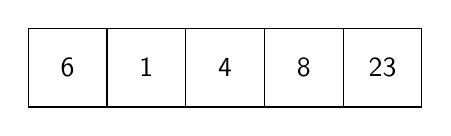
\begin{tikzpicture}[node distance=0cm, font=\sffamily, every node/.style={minimum width=1cm, minimum height=1cm, outer sep=0pt, anchor = west}, line join=miter, line cap=rect]
        \node[draw, fill=white] at (9, 0) {6};
        \node[draw, fill=white] at (10, 0) {1};
        \node[draw, fill=white] at (11, 0) {4};
        \node[draw, fill=white] at (12, 0) {8};
        \node[draw, fill=white] at (13, 0) {23};
    \end{tikzpicture}
\end{center}

\textbf{Bước 1:} Bắt đầu từ phần tử đầu tiên tại vị trí $i=0$, 
tìm phần tử nhỏ nhất trong phần mảng chưa sắp xếp $(1)$ và 
hoán vị với phần tử hiện tại $(6)$.

\begin{center}
    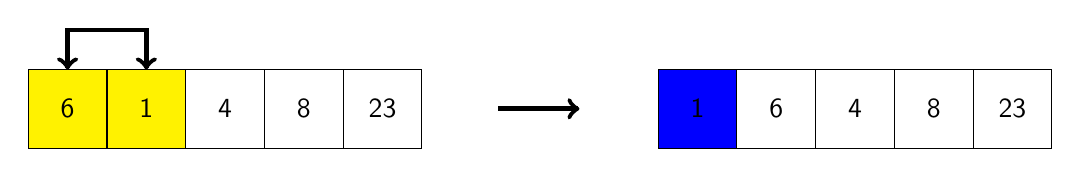
\begin{tikzpicture}[node distance=0cm, font=\sffamily, every node/.style={minimum width=1cm, minimum height=1cm, outer sep=0pt, anchor = west}, line join=miter, line cap=rect]
        \node[draw, fill=yellow] at (1, -3.5) {6};
        \node[draw, fill=yellow] at (2, -3.5) {1};
        \node[draw, fill=white] at (3, -3.5) {4};
        \node[draw, fill=white] at (4, -3.5) {8};
        \node[draw, fill=white] at (5, -3.5) {23};
        \draw[<-, line width=0.6mm, shorten <=0pt] (2.5, -3) -- (2.5, -2.5);
        \draw[line width=0.6mm] (2.5, -2.5) -- (1.5, -2.5);
        \draw[->, line width=0.6mm, shorten >=0pt] (1.5, -2.5) -- (1.5, -3);
        
        \draw[->, line width=0.6mm] (7, -3.5) -- (8, -3.5);
        
        \node[draw, fill=blue] at (9, -3.5) {1};
        \node[draw, fill=white] at (10, -3.5) {6};
        \node[draw, fill=white] at (11, -3.5) {4};
        \node[draw, fill=white] at (12, -3.5) {8};
        \node[draw, fill=white] at (13, -3.5) {23};
    \end{tikzpicture}
\end{center}
	
\textbf{Bước 2:} Chuyển đến phần tử tiếp theo tại vị trí $i=1$, 
tìm phần tử nhỏ nhất trong phần mảng chưa sắp xếp $(4)$ và 
hoán vị với phần tử hiện tại $(6)$.

\begin{center}
    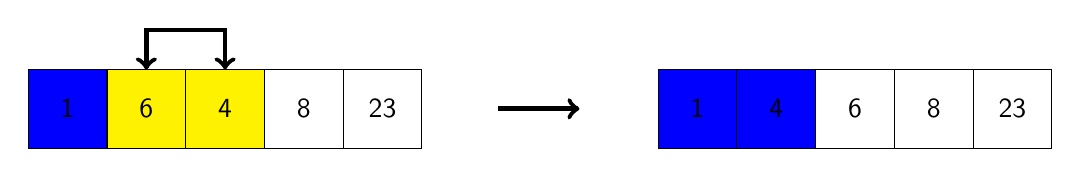
\begin{tikzpicture}[node distance=0cm, font=\sffamily, every node/.style={minimum width=1cm, minimum height=1cm, outer sep=0pt, anchor = west}, line join=miter, line cap=rect]
        \node[draw, fill=blue] at (1, -7) {1};
        \node[draw, fill=yellow] at (2, -7) {6};
        \node[draw, fill=yellow] at (3, -7) {4};
        \node[draw, fill=white] at (4, -7) {8};
        \node[draw, fill=white] at (5, -7) {23};
        \draw[<-, line width=0.6mm, shorten <=0pt] (3.5, -6.5) -- (3.5, -6);
        \draw[line width=0.6mm] (3.5, -6) -- (2.5, -6);
        \draw[->, line width=0.6mm, shorten >=0pt] (2.5, -6) -- (2.5, -6.5);
        
        \draw[->, line width=0.6mm] (7, -7) -- (8, -7);
        
        \node[draw, fill=blue] at (9, -7) {1};
        \node[draw, fill=blue] at (10, -7) {4};
        \node[draw, fill=white] at (11, -7) {6};
        \node[draw, fill=white] at (12, -7) {8};
        \node[draw, fill=white] at (13, -7) {23};
    \end{tikzpicture}
\end{center}

Do phần còn lại của mảng đã theo thứ tự nên các bước tiếp theo sẽ 
không có sự thay đổi và cuối cùng ta được mảng đã sắp xếp:

\begin{center}
    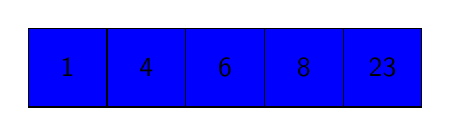
\begin{tikzpicture}[node distance=0cm, font=\sffamily, every node/.style={minimum width=1cm, minimum height=1cm, outer sep=0pt, anchor = west}, line join=miter, line cap=rect]
        \node[draw, fill=blue] at (0, 0) {1};
        \node[draw, fill=blue] at (1, 0) {4};
        \node[draw, fill=blue] at (2, 0) {6};
        \node[draw, fill=blue] at (3, 0) {8};
        \node[draw, fill=blue] at (4, 0) {23};
    \end{tikzpicture}
\end{center}

\subsubsection{Độ phức tạp thuật toán \textnormal{\cite{code-selection}}}

\begin{itemize}
    \item Độ phức tạp thời gian
    \begin{itemize}[label=$\circ$]
        \item Trường hợp tốt nhất: $O\left(n^2\right)$.
        \item Trường hợp xấu nhất: $O\left(n^2\right)$.
        \item Trung bình: $O\left(n^2\right)$ vì thuật toán sử dụng 
        hai vòng lặp lồng nhau để tìm phần tử nhỏ nhất.
    \end{itemize}
    \item Độ phức tạp không gian: $O\left(1\right)$ vì không sử dụng 
    bộ nhớ bổ sung ngoài danh sách ban đầu.
\end{itemize}
\subsection{Bubble Sort}

\subsubsection{Ý tưởng}

Trong thuật toán này, dãy các phần tử sẽ được duyệt từ đầu mảng đến 
cuối mảng, nếu hai phần tử kề nhau bị sai thứ tự thì đổi chỗ của chúng 
cho nhau. Sau lượt duyệt như vậy, phần tử lớn nhất sẽ được chuyển về 
vị trí cuối mảng giống như tên gọi - “nổi bọt”. Sau đó ta tiếp tục 
duyệt từ đầu mảng đến vị trí kế cuối mảng,... cứ như vậy cho đến khi 
mảng được sắp xếp.

\subsubsection{Mã giả}

\begin{algorithm}[H]
	\caption{Bubble Sort}
	\SetKwFunction{BubbleSort}{BubbleSort}
	\SetKwProg{Fn}{procedure}{:}{}
	\Fn{\BubbleSort{a\KwSty{[ ]}, n}}{
		\For{$i \gets 0$ \KwTo $n - 2$}{
			\For{$j \gets 0$ \KwTo $n - i - 2$}{
				\If{$a[j] > a[j + 1]$}{
					swap($a[j]$, $a[j + 1]$) \tcp{Nếu sai vị trí thì hoán vị}
				}
			}
		}
	}
\end{algorithm}

\subsubsection{Ví dụ}

\begin{tikzpicture}[node distance=0cm, scale=0.8, font=\sffamily, every node/.style={minimum width=0.8cm, minimum height=0.8cm, outer sep=0pt, anchor = west}, line join=miter, line cap=rect]
	
	% Trạng thái ban đầu
	\node[font=\rmfamily] at (0, 0) {Giả sử ta có mảng ban đầu với $n=5$ như sau:};
	\node[draw, fill=white] at (11, 0) {5};
	\node[draw, fill=white] at (12, 0) {3};
	\node[draw, fill=white] at (13, 0) {8};
	\node[draw, fill=white] at (14, 0) {6};
	\node[draw, fill=white] at (15, 0) {2};
	
	% Lượt duyệt 1
	% Cặp 1
	\node[font=\rmfamily] at (0, -1) {\bfseries Lượt duyệt 1:};
	\node[draw, fill=yellow] at (1, -3.5) {5};
	\node[draw, fill=yellow] at (2, -3.5) {3};
	\node[draw, fill=white] at (3, -3.5) {8};
	\node[draw, fill=white] at (4, -3.5) {6};
	\node[draw, fill=white] at (5, -3.5) {2};
	\draw[<-, line width=0.6mm, shorten <=0pt] (2.5, -3) -- (2.5, -2.5);
	\draw[line width=0.6mm] (2.5, -2.5) -- (1.5, -2.5);
	\draw[->, line width=0.6mm, shorten >=0pt] (1.5, -2.5) -- (1.5,-3);
	\node[font=\rmfamily, anchor=center] at (2, -2) {hoán vị};
	
	\draw[->, line width=0.6mm] (7, -3.5) -- (8, -3.5);
	
	% Cặp 2
	\node[draw, fill=white] at (9, -3.5) {3};
	\node[draw, fill=yellow] at (10, -3.5) {5};
	\node[draw, fill=yellow] at (11, -3.5) {8};
	\node[draw, fill=white] at (12, -3.5) {6};
	\node[draw, fill=white] at (13, -3.5) {2};
	\draw[<-, line width=0.6mm, shorten <=0pt] (11.5, -3) -- (11.5, -2.5);
	\draw[line width=0.6mm] (11.5, -2.5) -- (10.5, -2.5);
	\draw[->, line width=0.6mm, shorten >=0pt] (10.5, -2.5) -- (10.5,-3);
	\node[font=\rmfamily, anchor=center] at (11, -2) {không hoán vị};
	
	\draw[->, line width=0.6mm] (15, -3.5) -- (16, -3.5);
	
	% Cặp 3
	\node[draw, fill=white] at (17, -3.5) {3};
	\node[draw, fill=white] at (18, -3.5) {5};
	\node[draw, fill=yellow] at (19, -3.5) {8};
	\node[draw, fill=yellow] at (20, -3.5) {6};
	\node[draw, fill=white] at (21, -3.5) {2};
	\draw[<-, line width=0.6mm, shorten <=0pt] (20.5, -3) -- (20.5, -2.5);
	\draw[line width=0.6mm] (20.5, -2.5) -- (19.5, -2.5);
	\draw[->, line width=0.6mm, shorten >=0pt] (19.5, -2.5) -- (19.5,-3);
	\node[font=\rmfamily, anchor=center] at (20, -2) {hoán vị};
	
	\draw[->, line width=0.6mm] (7, -6.5) -- (8, -6.5);
	
	% Cặp 4
	\node[draw, fill=white] at (9, -6.5) {3};
	\node[draw, fill=white] at (10, -6.5) {5};
	\node[draw, fill=white] at (11, -6.5) {6};
	\node[draw, fill=yellow] at (12, -6.5) {8};
	\node[draw, fill=yellow] at (13, -6.5) {2};
	\draw[<-, line width=0.6mm, shorten <=0pt] (13.5, -6) -- (13.5, -5.5);
	\draw[line width=0.6mm] (13.5, -5.5) -- (12.5, -5.5);
	\draw[->, line width=0.6mm, shorten >=0pt] (12.5, -5.5) -- (12.5,-6);
	\node[font=\rmfamily, anchor=center] at (13, -5) {hoán vị};
	
	\draw[->, line width=0.6mm] (15, -6.5) -- (16, -6.5);
	
	% số 8 đúng vị trí
	\node[draw, fill=white] at (17, -6.5) {3};
	\node[draw, fill=white] at (18, -6.5) {5};
	\node[draw, fill=white] at (19, -6.5) {6};
	\node[draw, fill=white] at (20, -6.5) {2};
	\node[draw, fill=blue] at (21, -6.5) {8};
	
\end{tikzpicture}

%\pagebreak

\begin{tikzpicture}[node distance=0cm, scale=0.8, font=\sffamily, every node/.style={minimum width=0.8cm, minimum height=0.8cm, outer sep=0pt, anchor = west}, line join=miter, line cap=rect]
	% Lượt duyệt 2
	% Cặp 1
	\node[font=\rmfamily] at (0, 0) {\bfseries Lượt duyệt 2:};
	\node[draw, fill=yellow] at (1, -2.5) {3};
	\node[draw, fill=yellow] at (2, -2.5) {5};
	\node[draw, fill=white] at (3, -2.5) {6};
	\node[draw, fill=white] at (4, -2.5) {2};
	\node[draw, fill=blue] at (5, -2.5) {8};
	\draw[<-, line width=0.6mm, shorten <=0pt] (2.5, -2) -- (2.5, -1.5);
	\draw[line width=0.6mm] (2.5, -1.5) -- (1.5, -1.5);
	\draw[->, line width=0.6mm, shorten >=0pt] (1.5, -1.5) -- (1.5,-2);
	\node[font=\rmfamily, anchor=center] at (2, -1) {không hoán vị};
	
	\draw[->, line width=0.6mm] (7, -2.5) -- (8, -2.5);
	
	% Cặp 2
	\node[draw, fill=white] at (9, -2.5) {3};
	\node[draw, fill=yellow] at (10, -2.5) {5};
	\node[draw, fill=yellow] at (11, -2.5) {8};
	\node[draw, fill=white] at (12, -2.5) {6};
	\node[draw, fill=blue] at (13, -2.5) {2};
	\draw[<-, line width=0.6mm, shorten <=0pt] (11.5, -2) -- (11.5, -1.5);
	\draw[line width=0.6mm] (11.5, -1.5) -- (10.5, -1.5);
	\draw[->, line width=0.6mm, shorten >=0pt] (10.5, -1.5) -- (10.5,-2);
	\node[font=\rmfamily, anchor=center] at (11, -1) {không hoán vị};
	
	\draw[->, line width=0.6mm] (15, -2.5) -- (16, -2.5);
	
	% Cặp 3
	\node[draw, fill=white] at (17, -2.5) {3};
	\node[draw, fill=white] at (18, -2.5) {5};
	\node[draw, fill=yellow] at (19, -2.5) {6};
	\node[draw, fill=yellow] at (20, -2.5) {2};
	\node[draw, fill=blue] at (21, -2.5) {8};
	\draw[<-, line width=0.6mm, shorten <=0pt] (20.5, -2) -- (20.5, -1.5);
	\draw[line width=0.6mm] (20.5, -1.5) -- (19.5, -1.5);
	\draw[->, line width=0.6mm, shorten >=0pt] (19.5, -1.5) -- (19.5,-2);
	\node[font=\rmfamily, anchor=center] at (20, -1) {hoán vị};
	
	\draw[->, line width=0.6mm] (15, -4.5) -- (16, -4.5);
	
	% số 6,8 đúng vị trí
	\node[draw, fill=white] at (17, -4.5) {3};
	\node[draw, fill=white] at (18, -4.5) {5};
	\node[draw, fill=white] at (19, -4.5) {2};
	\node[draw, fill=blue] at (20, -4.5) {6};
	\node[draw, fill=blue] at (21, -4.5) {8};
	
	\node[font=\rmfamily] at (0, -6) {Cứ như vậy cho đến khi mảng được sắp xếp:};
	\node[draw, fill=blue] at (11, -6) {2};
	\node[draw, fill=blue] at (12, -6) {3};
	\node[draw, fill=blue] at (13, -6) {5};
	\node[draw, fill=blue] at (14, -6) {6};
	\node[draw, fill=blue] at (15, -6) {8};
	
\end{tikzpicture}

\subsubsection{Độ phức tạp thuật toán}

\begin{itemize}
    \item Độ phức tạp thời gian
    
    Trong thuật toán này, có $n-1$ lần lặp đối với biến $i$, mỗi lần 
    sẽ đưa phần tử lớn nhất trong đoạn $a\left[0..n-i-1\right]$ về 
    vị trí $n-i-1$. Với lần lặp thứ $i$, ta thực hiện $n-i$ 
    thao tác so sánh. Do đó, tổng số phép so sánh thực hiện là:
    
    \begin{equation*}
        \left(n-1\right)+\left(n-2\right)+\ldots+2+1
        =\frac{n\left(n-1\right)}{2}\approx n^2
    \end{equation*}
        
    Có thể thấy thuật toán không phụ thuộc vào phân bố ban đầu của dữ 
    liệu, ta có:
    
    \begin{itemize}[label=$\circ$]
        \item Trường hợp tốt nhất: $O\left(n^2\right)$.
        \item Trường hợp xấu nhất: $O\left(n^2\right)$.
        \item Trường hợp trung bình: $O\left(n^2\right)$.
    \end{itemize}
    
    \item Độ phức tạp không gian: $O\left(1\right)$.
\end{itemize}
\input{content/algo/3_shaker}
\subsection{Insertion Sort}

%Là thuật toán sắp xếp dựa trên phương pháp chèn trực tiếp. Thuật toán hoạt động hiệu quả trên mảng nhỏ hoặc mảng gần như đã sắp xếp.

\subsubsection{Ý tưởng}

Thuật toán này chia mảng thành hai phần: phần đã sắp xếp và 
phần chưa sắp xếp. Với mỗi phần tử trong mảng chưa sắp xếp, thuật toán chèn nó vào vị trí thích hợp trong phần đã sắp xếp. \cite[p.~90]{hoang2008}

\subsubsection{Mã giả}

\begin{algorithm}[H]
\caption{Insertion Sort \cite{code-insertion}}
\SetKwFunction{InsertionSort}{InsertionSort}
\SetKwProg{Fn}{Function}{:}{}
\Fn{\InsertionSort{a\KwSty{[]}, n}}{
    \For{$i \gets 1$ \KwTo $n - 1$}{
        $key \gets a[i]$ \\
        $j \gets i - 1$ \\
        \While{$j \geq 0$ \KwSty{and} $a[j] > key$}{
            // Di chuyển phần tử lớn hơn sang phải \\
            $a[j + 1] \gets a[j]$ \\
            $j \gets j - 1$ \\
        }
        // Chèn key vào đúng vị trí \\
        $a[j + 1] \gets key$
    }
}
\textbf{end function}
\end{algorithm}

\subsubsection{Ví dụ}

\begin{tikzpicture}[node distance=0cm, font=\sffamily, every node/.style={minimum width=1cm, minimum height=1cm, outer sep=0pt, anchor = west}, line join=miter, line cap=rect]
	
	% Trạng thái ban đầu
	\node[font=\rmfamily] at (0, 0) {Giả sử ta có mảng ban đầu với $n=6$ như sau:};
	\node[draw, fill=white] at (9, 0) {6};
	\node[draw, fill=white] at (10, 0) {1};
	\node[draw, fill=white] at (11, 0) {4};
	\node[draw, fill=white] at (12, 0) {8};
	\node[draw, fill=white] at (13, 0) {2};
	\node[draw, fill=white] at (14, 0) {15};
	
	% Trạng thái 1
	\node[font=\rmfamily] at (0, -1) {{\bfseries Bước 1:} Bắt đầu từ vị trí $i=1$, chèn 1 vào đúng vị trí của phần mảng đã sắp xếp (chỉ có 6).};
	\node[draw, fill=white] at (1, -2.5) {6};
	\node[draw, fill=yellow] at (2, -2.5) {1};
	\node[draw, fill=white] at (3, -2.5) {4};
	\node[draw, fill=white] at (4, -2.5) {8};
	\node[draw, fill=white] at (5, -2.5) {2};
	\node[draw, fill=white] at (6, -2.5) {15};
	\draw[line width=0.7mm, shorten <=0pt] (2.5, -2) -- (2.5, -1.5);
	\draw[line width=0.7mm] (2.5, -1.5) -- (1, -1.5);
	\draw[->, line width=0.7mm, shorten >=0pt] (1, -1.5) -- (1,-2);
	
	\draw[->, line width=0.7mm] (8, -2.5) -- (9.5, -2.5);
	
	\node[draw, fill=blue] at (10.5, -2.5) {1};
	\node[draw, fill=blue] at (11.5, -2.5) {6};
	\node[draw, fill=white] at (12.5, -2.5) {4};
	\node[draw, fill=white] at (13.5, -2.5) {8};
	\node[draw, fill=white] at (14.5, -2.5) {2};
	\node[draw, fill=white] at (15.5, -2.5) {15};
	
	% Trạng thái 2
	\node[font=\rmfamily] at (0, -4) {{\bfseries Bước 2:} Với vị trí $i=2$, chèn 4 vào đúng vị trí của phần mảng đã sắp xếp (gồm 1, 6).};
	\node[draw, fill=white] at (1, -5.5) {1};
	\node[draw, fill=white] at (2, -5.5) {6};
	\node[draw, fill=yellow] at (3, -5.5) {4};
	\node[draw, fill=white] at (4, -5.5) {8};
	\node[draw, fill=white] at (5, -5.5) {2};
	\node[draw, fill=white] at (6, -5.5) {15};
	\draw[line width=0.7mm, shorten <=0pt] (3.5, -5) -- (3.5, -4.5);
	\draw[line width=0.7mm] (3.5, -4.5) -- (2, -4.5);
	\draw[->, line width=0.7mm, shorten >=0pt] (2, -4.5) -- (2,-5);
	
	\draw[->, line width=0.7mm] (8, -5.5) -- (9.5, -5.5);
	
	\node[draw, fill=blue] at (10.5, -5.5) {1};
	\node[draw, fill=blue] at (11.5, -5.5) {4};
	\node[draw, fill=blue] at (12.5, -5.5) {6};
	\node[draw, fill=white] at (13.5, -5.5) {8};
	\node[draw, fill=white] at (14.5, -5.5) {2};
	\node[draw, fill=white] at (15.5, -5.5) {15};
		
\end{tikzpicture}

\begin{tikzpicture}[node distance=0cm, font=\sffamily, every node/.style={minimum width=1cm, minimum height=1cm, outer sep=0pt, anchor = west}, line join=miter, line cap=rect]
	
	% Trạng thái 3
	\node[font=\rmfamily, text width=18cm] at (0, 0) {{\bfseries Bước 3:} Với $i=3$, không thay đổi vị trí của 8 vì nó lớn hơn tất cả phần tử trong phần mảng \par đã sắp xếp.};
	\node[draw, fill=white] at (1, -1.5) {1};
	\node[draw, fill=white] at (2, -1.5) {4};
	\node[draw, fill=white] at (3, -1.5) {6};
	\node[draw, fill=yellow] at (4, -1.5) {8};
	\node[draw, fill=white] at (5, -1.5) {2};
	\node[draw, fill=white] at (6, -1.5) {15};
	\draw[line width=0.7mm, shorten <=0pt] (4.5, -1) -- (4.5, -0.5);
	\draw[line width=0.7mm] (4.5, -0.5) -- (4, -0.5);
	\draw[->, line width=0.7mm, shorten >=0pt] (4, -0.5) -- (4, -1);
	
	\draw[->, line width=0.7mm] (8, -1.5) -- (9.5, -1.5);
	
	\node[draw, fill=blue] at (10.5, -1.5) {1};
	\node[draw, fill=blue] at (11.5, -1.5) {4};
	\node[draw, fill=blue] at (12.5, -1.5) {6};
	\node[draw, fill=blue] at (13.5, -1.5) {8};
	\node[draw, fill=white] at (14.5, -1.5) {2};
	\node[draw, fill=white] at (15.5, -1.5) {15};
	
	% Trạng thái 4
	\node[font=\rmfamily, text width=20cm] at (0, -3) {{\bfseries Bước 4:} Tương tự, với $i=4$, chèn 2 vào đúng vị trí.};
	\node[draw, fill=white] at (1, -4.5) {1};
	\node[draw, fill=white] at (2, -4.5) {4};
	\node[draw, fill=white] at (3, -4.5) {6};
	\node[draw, fill=white] at (4, -4.5) {8};
	\node[draw, fill=yellow] at (5, -4.5) {2};
	\node[draw, fill=white] at (6, -4.5) {15};
	\draw[line width=0.7mm, shorten <=0pt] (5.5, -4) -- (5.5, -3.5);
	\draw[line width=0.7mm] (5.5, -3.5) -- (2, -3.5);
	\draw[->, line width=0.7mm, shorten >=0pt] (2, -3.5) -- (2, -4);
	
	\draw[->, line width=0.7mm] (8, -4.5) -- (9.5, -4.5);
	
	\node[draw, fill=blue] at (10.5, -4.5) {1};
	\node[draw, fill=blue] at (11.5, -4.5) {2};
	\node[draw, fill=blue] at (12.5, -4.5) {4};
	\node[draw, fill=blue] at (13.5, -4.5) {6};
	\node[draw, fill=blue] at (14.5, -4.5) {8};
	\node[draw, fill=white] at (15.5, -4.5) {15};
	
	% Trạng thái 5
	\node[font=\rmfamily, text width=20cm] at (0, -6) {{\bfseries Bước 5:} Cuối cùng, sau khi chèn 15 vào đúng vị trí, ta thu được mảng đã sắp xếp.};
	\node[draw, fill=white] at (1, -7.5) {1};
	\node[draw, fill=white] at (2, -7.5) {4};
	\node[draw, fill=white] at (3, -7.5) {6};
	\node[draw, fill=white] at (4, -7.5) {8};
	\node[draw, fill=white] at (5, -7.5) {2};
	\node[draw, fill=yellow] at (6, -7.5) {15};
	\draw[line width=0.7mm, shorten <=0pt] (6.5, -7) -- (6.5, -6.5);
	\draw[line width=0.7mm] (6.5, -6.5) -- (6, -6.5);
	\draw[->, line width=0.7mm, shorten >=0pt] (6, -6.5) -- (6, -7);
	
	\draw[->, line width=0.7mm] (8, -7.5) -- (9.5, -7.5);
	
	\node[draw, fill=blue] at (10.5, -7.5) {1};
	\node[draw, fill=blue] at (11.5, -7.5) {2};
	\node[draw, fill=blue] at (12.5, -7.5) {4};
	\node[draw, fill=blue] at (13.5, -7.5) {6};
	\node[draw, fill=blue] at (14.5, -7.5) {8};
	\node[draw, fill=blue] at (15.5, -7.5) {15};
	
\end{tikzpicture}

\subsubsection{Độ phức tạp thuật toán}

\begin{itemize}
    \item Độ phức tạp thời gian \cite[p.~91]{hoang2008}
    \begin{itemize}[label=$\circ$]
        \item Trường hợp tốt nhất: $O\left(n\right)$ khi mảng đã được sắp xếp.
        \item Trường hợp xấu nhất: $O\left(n^2\right)$ khi mảng sắp xếp 
        ngược, cần dịch chuyển toàn bộ phần tử cho mỗi lần chèn.
        \item Trường hợp trung bình: $O\left(n^2\right)$ do phải thực 
        hiện n lần chèn và mỗi lần chèn có thể phải dịch chuyển trung 
        bình n/2 phần tử.
    \end{itemize}
    \item Độ phức tạp không gian: $O\left(1\right)$ vì là thuật toán 
    sắp xếp tại chỗ (in-place), không sử dụng bộ nhớ phụ ngoài biến tạm.
\end{itemize}

\subsubsection{Các cải tiến của thuật toán}

\begin{enumerate}
    \item Binary Insertion Sort
    \begin{itemize}
        \item Ý tưởng: Thay vì sử dụng tìm kiếm tuyến tính để tìm vị trí 
        chèn phù hợp trong mảng đã sắp xếp thì ta có thể sử dụng thuật 
        toán làm việc được trên mảng đã sắp xếp để có thể tối ưu việc 
        tìm vị trí phù hợp để chèn. Đó chính là Binary Search để có 
        thể tìm kiếm tốt hơn với độ phức tạp của thuật toán là 
        $O\left(\log{n}\right)$. \cite[p.~91]{hoang2008}
        \item Ví dụ: Trong mảng $A=\left[1,4,5,10,15,20,9,21\right]$. 
        Khi xét vị trí $i=7$, ta cần tìm vị trí phụ hợp để chèn 9 
        vào thì có thể dùng binary search trong mảng đã sắp xếp trước 
        đó $\left(\left[1,4,5,10,15,20\right]\right)$ để tìm vị trí thích hợp.
    \end{itemize}
    \item Library Sort (còn gọi là gapped insertion sort)
    \begin{itemize}
        \item Ý tưởng: Thuật toán này có thể sử dụng các khoảng trống 
        (gaps) trong mảng để chèn phần tử, giúp hạn chế việc dịch 
        chuyển quá nhiều khi chèn giúp tối ưu trong việc xử lí khi 
        mảng có rất nhiều phần tử. Khi khoảng trống hết, mảng sẽ được 
        mở rộng và phân bổ lại khoảng trống mới. Với độ phức tạp thời 
        gian trung bình của Library Sort là $O\left(n\log{n}\right)$.
        \item Ví dụ: Với mảng $A=\left[3,4,5,8,1,2\right]$. Sau khi 
        tạo mảng với khoảng trống và chèn 3, 4, 5, 8 thì mảng 
        như sau $\left[3,\_,4,5,8\right]$.
        \begin{itemize}[label=$\circ$]
            \item Như vậy, khi chèn 1 vào đúng vị trí thì sẽ sắp xếp 
            lại và điền vào khoảng trống $\left[1,3,4,5,8\right]$.
            \item Tiếp theo, chèn 2, mảng không còn vị trí nào sau 
            phần tử 3 thì khi chèn 2 thì lúc này khoảng trống sẽ hết 
            thì mảng sẽ được mở rộng và phân bổ lại khoảng trống mới. 
            Mảng lúc này sẽ là $\left[1,\_,\_,3,4,5,8\right]$ khi đó 
            khi chèn 2 vào thì sẽ sử dụng khoảng trống mới mở rộng 
            $\left[1,2,\_,3,4,5,8\right]$.
        \end{itemize}
    \end{itemize}
\end{enumerate}
\subsection{Shell Sort}

Là một thuật toán sắp xếp dựa trên sắp xếp chèn (Insertion Sort), được 
đặt theo tên của người phát minh, Donald Shell. Thuật toán này cải tiến 
sắp xếp chèn bằng cách cho phép so sánh và hoán đổi các phần tử cách xa 
nhau trước khi thu hẹp khoảng cách lại. Điều này giúp giảm thiểu số lần 
hoán đổi và dịch chuyển các phần tử. Đây là một thuật toán không ổn định, 
phần tử bằng nhau có thể bị đổi chỗ do hoán đổi các nhóm cách xa nhau.

\subsubsection{Ý tưởng}

\begin{enumerate}
    \item Thay vì sắp xếp toàn bộ danh sách một cách tuần tự, Shell Sort 
    chia danh sách thành các danh sách con với khoảng cách giữa các phần 
    tử được xác định bởi một giá trị gọi là khoảng.
    \item Thuật toán sử dụng sắp xếp chèn để sắp xếp các phần tử trong 
    từng danh sách con này.
    \item Sau mỗi vòng lặp, khoảng cách được thu nhỏ dần, cuối cùng trở 
    về 1, lúc này danh sách được sắp xếp hoàn chỉnh.
\end{enumerate}

\subsubsection{Mã giả}

\begin{algorithm}[H]
    \caption{Shell Sort}
    \SetKwFunction{ShellSort}{ShellSort}
    \SetKwProg{Fn}{procedure}{:}{}
    \Fn{\ShellSort{a\KwSty{[ ]}, n}}{
        $gap \gets n / 2$ \tcp{Khởi tạo khoảng cách}
        \While{$gap > 0$}{
            \For{$i \gets gap$ \KwTo $n - 1$}{
                $temp \gets a[i],\ j \gets i$ \\
                
                \tcp{Dịch chuyển các phần tử lớn hơn temp lên một khoảng}
                \While{$j \geq gap$ \KwSty{and} $a[j - gap] > temp$}{
                    $a[j] \gets a[j - gap]$ \\
                    $j \gets j - gap$
                }
                $a[j] \gets temp$ \tcp{Đặt temp vào đúng vị trí}
            }
            $gap \gets gap / 2$ \tcp{Giảm khoảng cách}
        }
    }
\end{algorithm}

\subsubsection{Ví dụ}

Giả sử ta có mảng ban đầu với $n=5$ như sau:
\begin{center}
    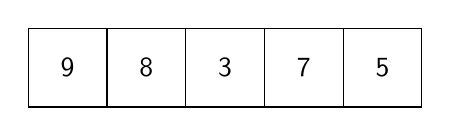
\begin{tikzpicture}[node distance=0cm, font=\sffamily, every node/.style={minimum width=1cm, minimum height=1cm, outer sep=0pt, anchor = west}, line join=miter, line cap=rect]
        \node[draw, fill=white] at (9, 0) {9};
        \node[draw, fill=white] at (10, 0) {8};
        \node[draw, fill=white] at (11, 0) {3};
        \node[draw, fill=white] at (12, 0) {7};
        \node[draw, fill=white] at (13, 0) {5};
    \end{tikzpicture}
\end{center}

Bắt đầu với $gap = 2$, thực hiện sắp xếp chèn với khoảng cách $gap$ 
cho từng phần tử từ vị trí $gap$ đến hết bên phải mảng.

\begin{center}
    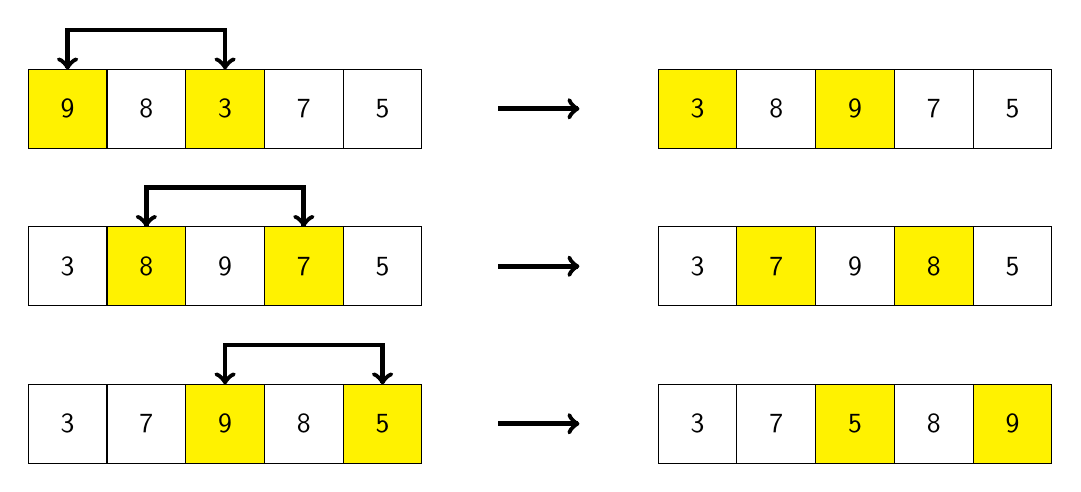
\begin{tikzpicture}[node distance=0cm, font=\sffamily, every node/.style={minimum width=1cm, minimum height=1cm, outer sep=0pt, anchor = west}, line join=miter, line cap=rect]
        % Substep 1
        \node[draw, fill=yellow] at (1, -3.5) {9};
        \node[draw, fill=white] at (2, -3.5) {8};
        \node[draw, fill=yellow] at (3, -3.5) {3};
        \node[draw, fill=white] at (4, -3.5) {7};
        \node[draw, fill=white] at (5, -3.5) {5};
        \draw[<-, line width=0.6mm, shorten <=0pt] (3.5, -3) -- (3.5, -2.5);
        \draw[line width=0.6mm] (3.5, -2.5) -- (1.5, -2.5);
        \draw[->, line width=0.6mm, shorten >=0pt] (1.5, -2.5) -- (1.5, -3);
        
        \draw[->, line width=0.6mm] (7, -3.5) -- (8, -3.5);
        
        \node[draw, fill=yellow] at (9, -3.5) {3};
        \node[draw, fill=white] at (10, -3.5) {8};
        \node[draw, fill=yellow] at (11, -3.5) {9};
        \node[draw, fill=white] at (12, -3.5) {7};
        \node[draw, fill=white] at (13, -3.5) {5};
        
        % Substep 2
        \node[draw, fill=white] at (1, -5.5) {3};
        \node[draw, fill=yellow] at (2, -5.5) {8};
        \node[draw, fill=white] at (3, -5.5) {9};
        \node[draw, fill=yellow] at (4, -5.5) {7};
        \node[draw, fill=white] at (5, -5.5) {5};
        \draw[<-, line width=0.6mm, shorten <=0pt] (4.5, -5) -- (4.5, -4.5);
        \draw[line width=0.6mm] (4.5, -4.5) -- (2.5, -4.5);
        \draw[->, line width=0.6mm, shorten >=0pt] (2.5, -4.5) -- (2.5, -5);
        
        \draw[->, line width=0.6mm] (7, -5.5) -- (8, -5.5);
        
        \node[draw, fill=white] at (9, -5.5) {3};
        \node[draw, fill=yellow] at (10, -5.5) {7};
        \node[draw, fill=white] at (11, -5.5) {9};
        \node[draw, fill=yellow] at (12, -5.5) {8};
        \node[draw, fill=white] at (13, -5.5) {5};
        
        % Substep 3
        \node[draw, fill=white] at (1, -7.5) {3};
        \node[draw, fill=white] at (2, -7.5) {7};
        \node[draw, fill=yellow] at (3, -7.5) {9};
        \node[draw, fill=white] at (4, -7.5) {8};
        \node[draw, fill=yellow] at (5, -7.5) {5};
        \draw[<-, line width=0.6mm, shorten <=0pt] (5.5, -7) -- (5.5, -6.5);
        \draw[line width=0.6mm] (5.5, -6.5) -- (3.5, -6.5);
        \draw[->, line width=0.6mm, shorten >=0pt] (3.5, -6.5) -- (3.5, -7);
        
        \draw[->, line width=0.6mm] (7, -7.5) -- (8, -7.5);
        
        \node[draw, fill=white] at (9, -7.5) {3};
        \node[draw, fill=white] at (10, -7.5) {7};
        \node[draw, fill=yellow] at (11, -7.5) {5};
        \node[draw, fill=white] at (12, -7.5) {8};
        \node[draw, fill=yellow] at (13, -7.5) {9};
    \end{tikzpicture}
\end{center}

Thực hiện tương tự với $gap = 1$, ta thu được mảng đã sắp xếp:

\begin{center}
    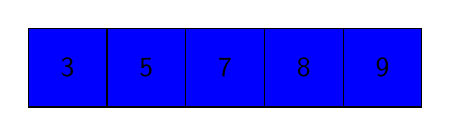
\begin{tikzpicture}[node distance=0cm, font=\sffamily, every node/.style={minimum width=1cm, minimum height=1cm, outer sep=0pt, anchor = west}, line join=miter, line cap=rect]
        \node[draw, fill=blue] at (9, 0) {3};
        \node[draw, fill=blue] at (10, 0) {5};
        \node[draw, fill=blue] at (11, 0) {7};
        \node[draw, fill=blue] at (12, 0) {8};
        \node[draw, fill=blue] at (13, 0) {9};
    \end{tikzpicture}
\end{center}

\subsubsection{Độ phức tạp thuật toán}

\begin{itemize}
    \item Độ phức tạp thời gian\\
    Hiệu suất của thuật toán Shell Sort phụ thuộc rất nhiều vào chuỗi 
    khoảng cách và thứ tự của mảng đầu vào (với chuỗi khoảng cách là tập 
    hợp tất cả các giá trị mà gap nhận trong quá trình thực hiện thuật 
    toán). Cụ thể:
    \begin{itemize}[label=$\circ$]
        \item Trường hợp tốt nhất: $O\left(n\log{n}\right)$, Khi mảng đầu vào 
        đã được sắp xếp hoàn toàn hoặc gần như sắp xếp và sử dụng một chuỗi 
        khoảng cách tối ưu (ví dụ: Knuth, Sedgewick,..). Vì khi mảng đã sắp 
        xếp, mỗi bước sắp xếp với khoảng cách gap chỉ cần thực hiện rất ít 
        phép so sánh và không cần hoán đổi. Còn chuỗi khoảng cách tối ưu đảm 
        bảo các phần tử được phân phối đều và nhanh chóng đưa mảng về trạng 
        thái sắp xếp hoàn chỉnh.

        \pagebreak

        \item Trường hợp xấu nhất: $O\left(n^2\right)$. Khi mảng đầu vào được 
        sắp xếp ngược và sử dụng chuỗi khoảng cách không tối ưu như $n,n/2,n/4,
        \ldots,1$, (giống trong mã giả nói trên). Trong trường hợp này, các 
        phần tử phải được di chuyển qua lại nhiều lần để đưa về đúng vị trí. 
        Đặc biệt, khi $gap = 1$, Shell Sort trở thành Insertion Sort, dẫn đến 
        hiệu suất tương tự là $O\left(n^2\right)$.
        \item Trường hợp trung bình: $O\left(n^{3/2}\right)$. Khi mảng đầu vào 
        có thứ tự ngẫu nhiên và sử dụng chuỗi khoảng cách phổ biến như $n,n/2,
        n/4,\ldots,1$. Trong trường hợp này, các phần tử không được phân phối 
        đều trong các lớp, dẫn đến việc cần thực hiện nhiều phép so sánh và 
        hoán đổi hơn. Đồng thời, với chuỗi khoảng cách không tối ưu, nhưng vẫn 
        đảm bảo hiệu suất tốt hơn so với Insertion Sort với độ phức tạp theo 
        thời gian trung bình là $O\left(n^2\right)$.
    \end{itemize}
    Lưu ý: Chuỗi khoảng cách là tập hợp tất cả các giá trị mà $gap$ nhận 
    trong quá trình thực hiện thuật toán.
    
    \item Độ phức tạp không gian: $O\left(1\right)$, vì Shell Sort là một 
    thuật toán in-place, nghĩa là nó không sử dụng bất kỳ cấu trúc dữ liệu 
    phụ nào ngoài một số biến tạm thời. Toàn bộ việc sắp xếp được thực hiện 
    trực tiếp trên mảng đầu vào. 
\end{itemize}
\subsection{Heap Sort}

\subsubsection{Ý tưởng}

\begin{itemize}
    \item Xây dựng Max-Heap: Chuyển đổi mảng đầu vào thành một Max-Heap, 
    sao cho phần tử lớn nhất nằm ở gốc cây.
    \item Sắp xếp:
    \begin{enumerate}
        \item Hoán đổi phần tử gốc (lớn nhất) với phần tử cuối cùng 
        của mảng.
        \item Giảm kích thước của heap đi 1 và gọi hàm Heapify để 
        duy trì tính chất Max-Heap.
        \item Lặp lại quá trình này cho đến khi heap chỉ còn một phần tử. \cite[p.~170]{cormen2022}
    \end{enumerate}
\end{itemize}

\subsubsection{Mã giả}

\begin{algorithm}[H]
\caption{Heap Sort \cite{code-heap}}
\SetKwFunction{Heapify}{heapify}
\SetKwFunction{HeapSort}{HeapSort}
\SetKwProg{Fn}{Function}{:}{}
\Fn{\Heapify{a\KwSty{[]}, n, i}}{
    $largest \gets i$ \\
    $left \gets 2 * i + 1$ \\
    $right \gets 2 * i + 2$ \\
    \If{$left < n$ \KwSty{and} $a[left] > a[largest]$}{
        $largest \gets left$ \\
    }
    \If{$right < n$ \KwSty{and} $a[right] > a[largest]$}{
        $largest \gets right$ \\
    }
    \If{$largest \neq i$}{
        // Đổi chỗ root với phần tử lớn nhất \\
        swap($a[i]$, $a[largest]$) \\
        // Đệ quy heapify trên node bị ảnh hưởng \\
        \Heapify{a, n, largest} \\
    }
}
\textbf{end function}

\Fn{\HeapSort{a\KwSty{[]}, n}}{
    // Bước 1: Xây dựng Max-Heap từ node trong cuối cùng \\
    \For{$i \gets \lfloor n / 2 \rfloor - 1$ \KwSty{downto} $0$}{
        \Heapify{a, n, i} \\
    }
    // Bước 2: Sắp xếp mảng bằng cách trích xuất các phần tử lớn nhất \\
    \For{$i \gets n - 1$ \KwSty{downto} $1$}{
        swap($a[0]$, $a[i]$) \\
        \Heapify{a, i, 0} \\
    }
}
\textbf{end function}
\end{algorithm}

\subsubsection{Ví dụ}

\begin{tikzpicture}[node distance=0cm, font=\sffamily, every node/.style={minimum width=1cm, minimum height=1cm, outer sep=0pt, anchor = west}, line join=miter, line cap=rect]
	
	% Trạng thái ban đầu
	\node[font=\rmfamily] at (0, 0) {Giả sử ta có mảng ban đầu với $n=6$ như sau:};
	\node[draw, fill=white] at (9, 0) {6};
	\node[draw, fill=white] at (10, 0) {1};
	\node[draw, fill=white] at (11, 0) {4};
	\node[draw, fill=white] at (12, 0) {8};
	\node[draw, fill=white] at (13, 0) {23};
	\node[draw, fill=white] at (14, 0) {2};
	
	% Build max-heap
	\node[font=\rmfamily] at (0, -1) {\bfseries Bước 1: Xây dựng max-heap};
	
	% Cặp 1
	\node[font=\rmfamily] at (0, -2) {$\bullet$ Bắt đầu với $i = \left\lfloor \dfrac{n}{2} \right\rfloor - 1 = 2$. So sánh 4 với 2, không xảy ra hoán vị.};
	\node[draw, fill=white] at (1, -3.5) {6};
	\node[draw, fill=white] at (2, -3.5) {1};
	\node[draw, fill=red!50] at (3, -3.5) {4};
	\node[draw, fill=white] at (4, -3.5) {8};
	\node[draw, fill=white] at (5, -3.5) {23};
	\node[draw, fill=yellow] at (6, -3.5) {2};
	
	% Cặp 2
	\node[font=\rmfamily] at (0, -5) {$\bullet$ Tiếp tục với $i = 1$. Lần lượt so sánh 1 với 8 và 23, hoán vị 1 với 23.};
	\node[draw, fill=white] at (1, -6) {6};
	\node[draw, fill=red!50] at (2, -6) {1};
	\node[draw, fill=white] at (3, -6) {4};
	\node[draw, fill=yellow] at (4, -6) {8};
	\node[draw, fill=yellow] at (5, -6) {23};
	\node[draw, fill=white] at (6, -6) {2};
	
	\draw[->, line width=0.5mm] (8, -6) -- (9, -6);
	
	\node[draw, fill=white] at (10, -6) {6};
	\node[draw, fill=red!50] at (11, -6) {23};
	\node[draw, fill=white] at (12, -6) {4};
	\node[draw, fill=yellow] at (13, -6) {8};
	\node[draw, fill=yellow] at (14, -6) {1};
	\node[draw, fill=white] at (15, -6) {2};
	
	% Cặp 3
	\node[font=\rmfamily] at (0, -7.5) {$\bullet$ Tiếp tục với $i = 0$. Lần lượt so sánh 6 với 23 và 4, hoán vị 6 với 23.};
	\node[draw, fill=red!50] at (1, -8.5) {6};
	\node[draw, fill=yellow] at (2, -8.5) {23};
	\node[draw, fill=yellow] at (3, -8.5) {4};
	\node[draw, fill=white] at (4, -8.5) {8};
	\node[draw, fill=white] at (5, -8.5) {1};
	\node[draw, fill=white] at (6, -8.5) {2};
	
	\draw[->, line width=0.5mm] (8, -8.5) -- (9, -8.5);
	
	\node[draw, fill=red!50] at (10, -8.5) {23};
	\node[draw, fill=yellow] at (11, -8.5) {6};
	\node[draw, fill=yellow] at (12, -8.5) {4};
	\node[draw, fill=white] at (13, -8.5) {8};
	\node[draw, fill=white] at (14, -8.5) {1};
	\node[draw, fill=white] at (15, -8.5) {2};
\end{tikzpicture}

\begin{tikzpicture}[node distance=0cm, font=\sffamily, every node/.style={minimum width=1cm, minimum height=1cm, outer sep=0pt, anchor = west}, line join=miter, line cap=rect]
	
	% Cặp 4
	\node[font=\rmfamily] at (0, -10) {$\bullet$ Hiệu chỉnh lan truyền: Lần lượt so sánh 6 với 8 và 1, hoán vị 6 với 8.};
	\node[draw, fill=white] at (1, -11) {23};
	\node[draw, fill=red!50] at (2, -11) {6};
	\node[draw, fill=white] at (3, -11) {4};
	\node[draw, fill=yellow] at (4, -11) {8};
	\node[draw, fill=yellow] at (5, -11) {1};
	\node[draw, fill=white] at (6, -11) {2};
	
	\draw[->, line width=0.5mm] (8, -11) -- (9, -11);
	
	\node[draw, fill=white] at (10, -11) {23};
	\node[draw, fill=red!50] at (11, -11) {8};
	\node[draw, fill=white] at (12, -11) {4};
	\node[draw, fill=yellow] at (13, -11) {6};
	\node[draw, fill=yellow] at (14, -11) {1};
	\node[draw, fill=white] at (15, -11) {2};
	
	% Sắp xếp
	\node[font=\rmfamily] at (0, -12.5) {\bfseries Bước 2: Sắp xếp mảng bằng cách lấy ra phần tử lớn nhất và heapify phần còn lại};
	
	% Phần tử 1
	\node[font=\rmfamily] at (0, -13.5) {$\bullet$ Hoán vị 23 với phần tử cuối cùng của heap, giảm kích thước heap xuống còn 5 và heapify lại.};
	\node[draw, fill=white] at (1, -14.5) {2};
	\node[draw, fill=white] at (2, -14.5) {8};
	\node[draw, fill=white] at (3, -14.5) {4};
	\node[draw, fill=white] at (4, -14.5) {6};
	\node[draw, fill=white] at (5, -14.5) {1};
	\node[draw, fill=blue] at (6, -14.5) {23};
	
	\draw[->, line width=0.5mm] (8, -14.5) -- (9, -14.5);
	
	\node[draw, fill=white] at (10, -14.5) {8};
	\node[draw, fill=white] at (11, -14.5) {6};
	\node[draw, fill=white] at (12, -14.5) {4};
	\node[draw, fill=white] at (13, -14.5) {2};
	\node[draw, fill=white] at (14, -14.5) {1};
	\node[draw, fill=blue] at (15, -14.5) {23};
	
	% Phần tử 2
	\node[font=\rmfamily] at (0, -16) {$\bullet$ Hoán vị 8 với phần tử cuối cùng của heap, giảm kích thước heap xuống còn 4 và heapify lại.};
	\node[draw, fill=white] at (1, -17) {1};
	\node[draw, fill=white] at (2, -17) {6};
	\node[draw, fill=white] at (3, -17) {4};
	\node[draw, fill=white] at (4, -17) {2};
	\node[draw, fill=blue] at (5, -17) {8};
	\node[draw, fill=blue] at (6, -17) {23};
	
	\draw[->, line width=0.5mm] (8, -17) -- (9, -17);
	
	\node[draw, fill=white] at (10, -17) {6};
	\node[draw, fill=white] at (11, -17) {2};
	\node[draw, fill=white] at (12, -17) {4};
	\node[draw, fill=white] at (13, -17) {1};
	\node[draw, fill=blue] at (14, -17) {8};
	\node[draw, fill=blue] at (15, -17) {23};
	
	% Phần tử 3
	\node[font=\rmfamily] at (0, -18.5) {$\bullet$ Hoán vị 6 với phần tử cuối cùng của heap, giảm kích thước heap xuống còn 3 và heapify lại.};
	\node[draw, fill=white] at (1, -19.5) {1};
	\node[draw, fill=white] at (2, -19.5) {2};
	\node[draw, fill=white] at (3, -19.5) {4};
	\node[draw, fill=blue] at (4, -19.5) {6};
	\node[draw, fill=blue] at (5, -19.5) {8};
	\node[draw, fill=blue] at (6, -19.5) {23};
	
	\draw[->, line width=0.5mm] (8, -19.5) -- (9, -19.5);
	
	\node[draw, fill=white] at (10, -19.5) {4};
	\node[draw, fill=white] at (11, -19.5) {2};
	\node[draw, fill=white] at (12, -19.5) {1};
	\node[draw, fill=blue] at (13, -19.5) {6};
	\node[draw, fill=blue] at (14, -19.5) {8};
	\node[draw, fill=blue] at (15, -19.5) {23};
	
	% Phần tử 4
	\node[font=\rmfamily] at (0, -21) {$\bullet$ Hoán vị 4 với phần tử cuối cùng của heap, giảm kích thước heap xuống còn 2 và heapify lại.};
	\node[draw, fill=white] at (1, -22) {1};
	\node[draw, fill=white] at (2, -22) {2};
	\node[draw, fill=blue] at (3, -22) {4};
	\node[draw, fill=blue] at (4, -22) {6};
	\node[draw, fill=blue] at (5, -22) {8};
	\node[draw, fill=blue] at (6, -22) {23};
	
	\draw[->, line width=0.5mm] (8, -22) -- (9, -22);
	
	\node[draw, fill=white] at (10, -22) {2};
	\node[draw, fill=white] at (11, -22) {1};
	\node[draw, fill=blue] at (12, -22) {4};
	\node[draw, fill=blue] at (13, -22) {6};
	\node[draw, fill=blue] at (14, -22) {8};
	\node[draw, fill=blue] at (15, -22) {23};
	
	% Phần tử 5
	\node[font=\rmfamily,  text width=10cm] at (0, -23.5) {$\bullet$ Hoán vị 2 với phần tử cuối cùng của heap, \par \hspace{0.35cm} ta thu được mảng đã sắp xếp:};
	\node[draw, fill=blue] at (9, -23.5) {1};
	\node[draw, fill=blue] at (10, -23.5) {2};
	\node[draw, fill=blue] at (11, -23.5) {4};
	\node[draw, fill=blue] at (12, -23.5) {6};
	\node[draw, fill=blue] at (13, -23.5) {8};
	\node[draw, fill=blue] at (14, -23.5) {23};
	
\end{tikzpicture}

\subsubsection{Độ phức tạp thuật toán}

\begin{itemize}
    \item Độ phức tạp thời gian \cite[p.~102]{hoang2008}
    \begin{itemize}[label=$\circ$]
        \item Trường hợp tốt nhất: $O(n\log{n})$ vì khi xây dựng heap 
        và thực hiện thao tác heapify vẫn cần $O(n \log n)$ do tính 
        chất của heap.
        \item Trường hợp xấu nhất: $O(n\log{n})$ trong trường hợp tệ 
        nhất (mảng hoàn toàn ngược hoặc có cấu trúc phức tạp) vẫn duy 
        trì $O(n \log n)$ vì mọi thao tác chính đều dựa trên việc 
        heapify từng phần tử.
        \item Trường hợp trung bình: $O(n\log{n})$ trường hợp trung bình 
        vẫn cần xây dựng heap và thực hiện $n-1$ lần thao tác Heapify.
    \end{itemize}
    \item Độ phức tạp không gian: $O(1)$ vì Heap Sort là thuật toán 
    sắp xếp tại chỗ (in-place), không sử dụng bộ nhớ phụ ngoài biến tạm.
\end{itemize}
\input{content/algo/7_merge}
\subsection{Quick Sort}

\subsubsection{Ý tưởng}

Để sắp xếp một đoạn trong mảng, nếu đoạn đó có ít hơn 2 phần tử thì không cần phải làm gì cả. Ngược lại, nếu đoạn đó có từ 2 phần tử trở lên, ta chọn một phần tử ở chính giữa làm “chốt” (pivot), sau đó phân hoạch thành 2 đoạn nhỏ hơn sao cho các phần tử ở đoạn bên trái không lớn hơn pivot và các phần tử ở đoạn bên phải không nhỏ hơn pivot. Tiếp theo, ta áp dụng phương pháp tương tự cho 2 mảng con đó bằng cách gọi đệ quy đến từng mảng. \cite{idea-quick} \cite[p.~93--94]{hoang2008}

\subsubsection{Mã giả}

\begin{algorithm}[H]
	\caption{Quick Sort \cite[p.~183--184]{cormen2022} \cite{code-quick}}
	\label{quick-sort}

	\SetKwFunction{QuickSort}{QuickSort}
	\SetKwProg{Fn}{procedure}{:}{}
	\Fn{\QuickSort {a\KwSty{[ ]}, left, right}}{
		$i \gets left$ \\
		$j \gets right$ \\
		$pivot = a[left + (right - left) / 2]$ \\
		\tcp{Phân hoạch thành 2 đoạn}
		\While{$i \leq j$}{ 
			\While{$a[i] < pivot$}{
				$++i$
			}
			\While{$a[j] > pivot$}{
				$--j$
			}
			\If{$i \leq j$}{
				swap($a[i]$, $a[j]$) \\
				$++i$ \\
				$--j$ 
			}
		}
		\tcp{Gọi đệ quy cho 2 mảng con}
		\If{$i < right$}{
			\QuickSort{a, i, right}
		}
		\If{$j > left$}{
			\QuickSort{a, left, j}
		}
	}
\end{algorithm}

\subsubsection{Ví dụ}

\begin{tikzpicture}[node distance=0cm, font=\sffamily, every node/.style={minimum width=1cm, minimum height=1cm, outer sep=0pt, anchor = west}, line join=miter, line cap=rect]
	
	% Trạng thái ban đầu
	\node[font=\rmfamily] at (0, 0) {Giả sử ta có mảng ban đầu với $n=7$ như sau:};
	\node[draw, fill=white] at (9, 0) {8};
	\node[draw, fill=white] at (10, 0) {3};
	\node[draw, fill=white] at (11, 0) {1};
	\node[draw, fill=white] at (12, 0) {7};
	\node[draw, fill=white] at (13, 0) {0};
	\node[draw, fill=white] at (14, 0) {10};
	\node[draw, fill=white] at (15, 0) {2};
	
	% Cặp 1
	\node[font=\rmfamily] at (0, -1) {{\bfseries Xét lần phân hoạch đầu tiên:} Theo mã giả, chọn $pivot = a[3] = 7$.};
	\node[font=\rmfamily] at (0, -2) {Với $i=0$ và $j=6$, ta có $a[i] = 8 \geq pivot$ và $a[j] = 2 \leq pivot \rightarrow$ {\bfseries Hoán vị}};
	\node[font=\rmfamily, anchor=center] at (4.5, -2.8) {\bfseries pivot};
	\node[draw, fill=yellow] at (1, -3.5) {8};
	\node[draw, fill=white] at (2, -3.5) {3};
	\node[draw, fill=white] at (3, -3.5) {1};
	\node[draw, fill=red!50] at (4, -3.5) {7};
	\node[draw, fill=white] at (5, -3.5) {0};
	\node[draw, fill=white] at (6, -3.5) {10};
	\node[draw, fill=yellow] at (7, -3.5) {2};
	\draw[<-, line width=0.7mm, shorten <=0pt] (7.5, -3) -- (7.5, -2.5);
	\draw[line width=0.7mm] (7.5, -2.5) -- (1.5, -2.5);
	\draw[->, line width=0.7mm, shorten >=0pt] (1.5, -2.5) -- (1.5,-3);
	
	
	% Cặp 2
	\node[font=\rmfamily] at (0, -5) {Tăng $i$ đến khi $i=3$, ta có $a[i] = 7 \geq pivot \rightarrow$ {\bfseries Dừng tăng $i$}};
	\node[draw, fill=blue] at (1, -6) {8};
	\node[draw, fill=blue] at (2, -6) {3};
	\node[draw, fill=blue] at (3, -6) {1};
	\node[draw, fill=yellow] at (4, -6) {7};
	\node[draw, fill=white] at (5, -6) {0};
	\node[draw, fill=white] at (6, -6) {10};
	\node[draw, fill=blue] at (7, -6) {2};
	
	% Cặp 3
	\node[font=\rmfamily] at (0, -7.5) {Giảm $j$ đến khi $j=4$, ta có $a[j] = 0 \leq pivot \rightarrow$ {\bfseries Dừng giảm $j$}};
	\node[draw, fill=blue] at (1, -8.5) {8};
	\node[draw, fill=blue] at (2, -8.5) {3};
	\node[draw, fill=blue] at (3, -8.5) {1};
	\node[draw, fill=yellow] at (4, -8.5) {7};
	\node[draw, fill=yellow] at (5, -8.5) {0};
	\node[draw, fill=blue] at (6, -8.5) {10};
	\node[draw, fill=blue] at (7, -8.5) {2};
	
	% Cặp cuối
	\node[font=\rmfamily] at (0, -10) {Với $i=3$ và $j=4$, ta có $a[i] = 7 \geq pivot$ và $a[j] = 0 \leq pivot \rightarrow$ {\bfseries Hoán vị}};
	\node[draw, fill=blue] at (1, -11.5) {2};
	\node[draw, fill=blue] at (2, -11.5) {3};
	\node[draw, fill=blue] at (3, -11.5) {1};
	\node[draw, fill=yellow] at (4, -11.5) {7};
	\node[draw, fill=yellow] at (5, -11.5) {0};
	\node[draw, fill=blue] at (6, -11.5) {10};
	\node[draw, fill=blue] at (7, -11.5) {8};
	\draw[<-, line width=0.7mm, shorten <=0pt] (5.5, -11) -- (5.5, -10.5);
	\draw[line width=0.7mm] (5.5, -10.5) -- (4.5, -10.5);
	\draw[->, line width=0.7mm, shorten >=0pt] (4.5, -10.5) -- (4.5,-11);
	
	% Kết thúc phân hoạch
	\node[font=\rmfamily] at (0, -13) {Với $i=4$ và $j=3$, ta có $i > j \rightarrow$ {\bfseries Kết thúc lần phân hoạch đầu tiên}};
	\node[draw, fill=blue] at (1, -14) {2};
	\node[draw, fill=blue] at (2, -14) {3};
	\node[draw, fill=blue] at (3, -14) {1};
	\node[draw, fill=blue] at (4, -14) {0};
	\node[draw, fill=blue] at (5.3, -14) {7};
	\node[draw, fill=blue] at (6.3, -14) {10};
	\node[draw, fill=blue] at (7.3, -14) {8};
	
	\node[font=\rmfamily] at (0, -15.5) {Thực hiện tương tự đối với các mảng con, ta thu được mảng đã sắp xếp.};
	\node[draw, fill=blue] at (1, -16.5) {0};
	\node[draw, fill=blue] at (2, -16.5) {1};
	\node[draw, fill=blue] at (3, -16.5) {2};
	\node[draw, fill=blue] at (4, -16.5) {3};
	\node[draw, fill=blue] at (5, -16.5) {7};
	\node[draw, fill=blue] at (6, -16.5) {8};
	\node[draw, fill=blue] at (7, -16.5) {10};
\end{tikzpicture}

\subsubsection{Độ phức tạp}

\begin{itemize}
    \item Độ phức tạp thời gian \cite[p.~209--212]{cormen2022}
    \begin{itemize}[label=$\circ$]
        \item Trường hợp tốt nhất: Giá trị pivot được chọn luôn là trung vị của dãy, do đó nó phân hoạch dãy thành 2 phần bằng nhau. Vì ở mỗi lần chia, kích thước mảng giảm đi một nửa nên khi đó sẽ có $log_2{n}$ mức đệ quy. Ở mỗi mức, thuật toán phải thao tác trên toàn bộ mảng nên có độ phức tạp là $O\left(n\right)$. Như vậy, tổng hợp độ phức tạp trong trường hợp này là $O\left(n\log{n}\right)$.
        
		\pagebreak

        \item Trường hợp xấu nhất: Giá trị pivot được chọn luôn là phần tử nhỏ nhất hoặc lớn nhất của dãy, do đó sau mỗi lần phân hoạch, một đoạn không có phần tử nào và đoạn còn lại có $n - 1$ phần tử. Khi đó, thuật toán phải thực hiện  $n - 1$ mức đệ quy, mỗi mức xử lý toàn bộ mảng còn lại với độ phức tạp $O\left(n\right)$. Như vậy, tổng hợp độ phức tạp trong trường hợp này là $O\left(n^2\right)$.
        
        \item Trường hợp trung bình: $O\left(n\log{n}\right)$ 
    \end{itemize}
    
    \item Độ phức tạp không gian: $O\left(1\right)$
\end{itemize}
\subsection{Counting Sort}

[TO DO]
\subsection{Radix Sort}

\subsubsection{Ý tưởng}

Radix Sort sắp xếp các phần tử bằng cách xử lý từng chữ số của các số từ hàng thấp nhất (hàng đơn vị) đến hàng cao nhất. Thuật toán này sử dụng Counting Sort như một bước phụ trợ để sắp xếp theo từng chữ số.

\subsubsection{Mã giả}

\begin{algorithm}[H]
    \caption{Radix Sort}
    \label{radix-sort}

    \SetKwFunction{CountingSortByDigit}{CountingSortByDigit}
    \SetKwProg{Fn}{procedure}{:}{}
    \Fn{\CountingSortByDigit {a\KwSty{[ ]}, n, exp}}{
        $count[10] \gets \{0\},\ output[n] \gets \{0\}$ \tcp{Khởi tạo mảng đếm và mảng kết quả}
        \For{$i \gets 0$ \KwTo $n-1$}{
            $index = (a[i]\ /\ exp)\ \%\ 10$ \\
            $count[index]++$
        }
        \For{$i \gets 1$ \KwTo $9$}{
            $count[i] += count[i-1]$
        }
        \For{$i \gets n-1$ \KwSty{downto} $0$}{
            $index = (a[i]\ /\ exp)\ \%\ 10$ \\
            $output[count[index] - 1] = a[i]$ \\
            $count[index]--$
        }
        \For{$i \gets 0$ \KwTo $n-1$}{
            $a[i] = output[i]$
        }
    }
\end{algorithm}

\begingroup
\renewcommand{\thealgocf}{} % Loại bỏ số thứ tự
\setlength{\algotitleheightrule}{0pt} % Loại bỏ dòng kẻ trên tiêu đề
\setlength{\interspacetitleruled}{0pt} % Không khoảng cách giữa tiêu đề và đường kẻ
\setlength{\interspacealgoruled}{0pt} % Không khoảng cách giữa đường kẻ và nội dung

\begin{algorithm}[H]
	\setcounter{AlgoLine}{13} % Tiếp tục số dòng từ phần trước
    \SetKwFunction{RadixSort}{RadixSort}
    \SetKwProg{Fn}{procedure}{:}{}
    \Fn{\RadixSort {a\KwSty{[ ]}, n}}{
        $maxVal \gets max(a,n)$ \tcp{Tìm giá trị lớn nhất để biết số chữ số}
        $exp \gets 1$ \\
        \While{$maxVal / exp > 0$}{
            \CountingSortByDigit{a, n, exp} \\
            $exp\ *=\ 10$
        }
    }
\end{algorithm}
\endgroup

\subsubsection{Ví dụ}

Giả sử ta có mảng ban đầu với $n=7$ như sau:
\begin{center}
    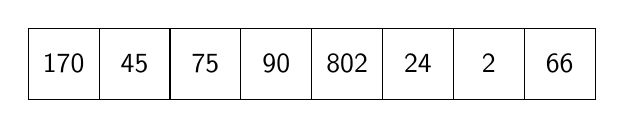
\begin{tikzpicture}[node distance=0cm, scale=0.9, font=\sffamily, every node/.style={minimum width=0.9cm, minimum height=0.9cm, outer sep=0pt, anchor = west}, line join=miter, line cap=rect]
        \node[draw, fill=white] at (9, 0) {170};
        \node[draw, fill=white] at (10, 0) {45};
        \node[draw, fill=white] at (11, 0) {75};
        \node[draw, fill=white] at (12, 0) {90};
        \node[draw, fill=white] at (13, 0) {802};
        \node[draw, fill=white] at (14, 0) {24};
        \node[draw, fill=white] at (15, 0) {2};
        \node[draw, fill=white] at (16, 0) {66};
    \end{tikzpicture}
\end{center}

\textbf{Bước 1:} Sắp xếp theo chữ số hàng đơn vị $(exp = 1)$.

\begin{center}
    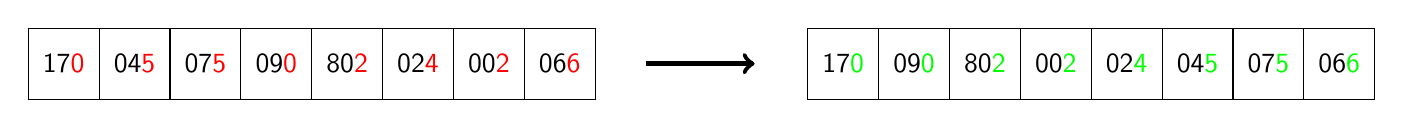
\begin{tikzpicture}[node distance=0cm, scale=0.9, font=\sffamily, every node/.style={minimum width=0.9cm, minimum height=0.9cm, outer sep=0pt, anchor = west}, line join=miter, line cap=rect]
        \node[draw, fill=white] at (0, 0) {17\textcolor{red}{0}};
        \node[draw, fill=white] at (1, 0) {04\textcolor{red}{5}};
        \node[draw, fill=white] at (2, 0) {07\textcolor{red}{5}};
        \node[draw, fill=white] at (3, 0) {09\textcolor{red}{0}};
        \node[draw, fill=white] at (4, 0) {80\textcolor{red}{2}};
        \node[draw, fill=white] at (5, 0) {02\textcolor{red}{4}};
        \node[draw, fill=white] at (6, 0) {00\textcolor{red}{2}};
        \node[draw, fill=white] at (7, 0) {06\textcolor{red}{6}};
        
        \draw[->, line width=0.6mm] (8.75, 0) -- (10.25, 0);
        
        \node[draw, fill=white] at (11, 0) {17\textcolor{green}{0}};
        \node[draw, fill=white] at (12, 0) {09\textcolor{green}{0}};
        \node[draw, fill=white] at (13, 0) {80\textcolor{green}{2}};
        \node[draw, fill=white] at (14, 0) {00\textcolor{green}{2}};
        \node[draw, fill=white] at (15, 0) {02\textcolor{green}{4}};
        \node[draw, fill=white] at (16, 0) {04\textcolor{green}{5}};
        \node[draw, fill=white] at (17, 0) {07\textcolor{green}{5}};
        \node[draw, fill=white] at (18, 0) {06\textcolor{green}{6}};
    \end{tikzpicture}
\end{center}

\textbf{Bước 2:} Sắp xếp theo chữ số hàng hàng chục $(exp = 10)$.

\begin{center}
    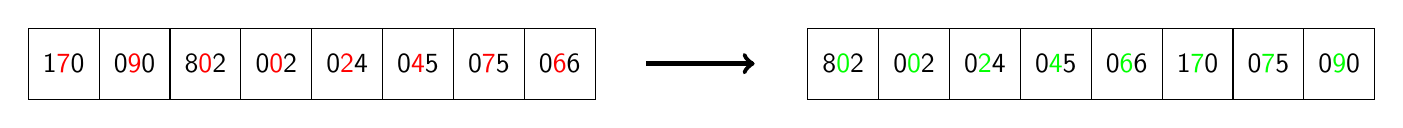
\begin{tikzpicture}[node distance=0cm, scale=0.9, font=\sffamily, every node/.style={minimum width=0.9cm, minimum height=0.9cm, outer sep=0pt, anchor = west}, line join=miter, line cap=rect]
        \node[draw, fill=white] at (0, 0) {1\textcolor{red}{7}0};
        \node[draw, fill=white] at (1, 0) {0\textcolor{red}{9}0};
        \node[draw, fill=white] at (2, 0) {8\textcolor{red}{0}2};
        \node[draw, fill=white] at (3, 0) {0\textcolor{red}{0}2};
        \node[draw, fill=white] at (4, 0) {0\textcolor{red}{2}4};
        \node[draw, fill=white] at (5, 0) {0\textcolor{red}{4}5};
        \node[draw, fill=white] at (6, 0) {0\textcolor{red}{7}5};
        \node[draw, fill=white] at (7, 0) {0\textcolor{red}{6}6};
        
        \draw[->, line width=0.6mm] (8.75, 0) -- (10.25, 0);
        
        \node[draw, fill=white] at (11, 0) {8\textcolor{green}{0}2};
        \node[draw, fill=white] at (12, 0) {0\textcolor{green}{0}2};
        \node[draw, fill=white] at (13, 0) {0\textcolor{green}{2}4};
        \node[draw, fill=white] at (14, 0) {0\textcolor{green}{4}5};
        \node[draw, fill=white] at (15, 0) {0\textcolor{green}{6}6};
        \node[draw, fill=white] at (16, 0) {1\textcolor{green}{7}0};
        \node[draw, fill=white] at (17, 0) {0\textcolor{green}{7}5};
        \node[draw, fill=white] at (18, 0) {0\textcolor{green}{9}0};
    \end{tikzpicture}
\end{center}

\textbf{Bước 3:} Sắp xếp theo chữ số hàng hàng trăm $(exp = 100)$.

\begin{center}
    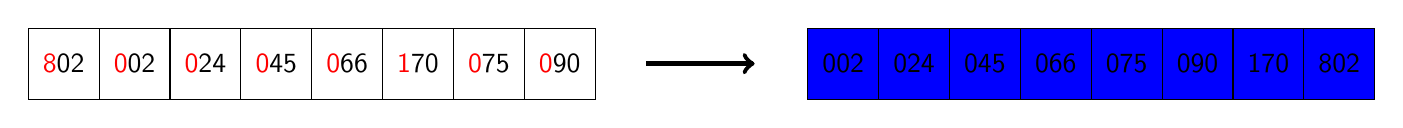
\begin{tikzpicture}[node distance=0cm, scale=0.9, font=\sffamily, every node/.style={minimum width=0.9cm, minimum height=0.9cm, outer sep=0pt, anchor = west}, line join=miter, line cap=rect]
        \node[draw, fill=white] at (0, 0) {\textcolor{red}{8}02};
        \node[draw, fill=white] at (1, 0) {\textcolor{red}{0}02};
        \node[draw, fill=white] at (2, 0) {\textcolor{red}{0}24};
        \node[draw, fill=white] at (3, 0) {\textcolor{red}{0}45};
        \node[draw, fill=white] at (4, 0) {\textcolor{red}{0}66};
        \node[draw, fill=white] at (5, 0) {\textcolor{red}{1}70};
        \node[draw, fill=white] at (6, 0) {\textcolor{red}{0}75};
        \node[draw, fill=white] at (7, 0) {\textcolor{red}{0}90};
        
        \draw[->, line width=0.6mm] (8.75, 0) -- (10.25, 0);
        
        \node[draw, fill=blue] at (11, 0) {002};
        \node[draw, fill=blue] at (12, 0) {024};
        \node[draw, fill=blue] at (13, 0) {045};
        \node[draw, fill=blue] at (14, 0) {066};
        \node[draw, fill=blue] at (15, 0) {075};
        \node[draw, fill=blue] at (16, 0) {090};
        \node[draw, fill=blue] at (17, 0) {170};
        \node[draw, fill=blue] at (18, 0) {802};
    \end{tikzpicture}
\end{center}

\subsubsection{Độ phức tạp thuật toán}

\begin{itemize}
    \item Độ phức tạp thời gian
    \begin{itemize}[label=$\circ$]
        \item Trường hợp tốt nhất: $O\left(d\times\left(n+k\right)\right)$. 
        Khi $n$ lớn và $k$ nhỏ. 
        \item Trường hợp xấu nhất: $O\left(d\times\left(n+k\right)\right)$. 
        Trường hợp xấu nhất xảy ra khi giá trị lớn nhất trong mảng có nhiều 
        chữ số $(d)$ lớn và phạm vi giá trị của mỗi chữ số $(k)$ lớn. Tuy nhiên, 
        hiệu suất vẫn được đảm bảo bởi tính ổn định của Counting Sort.
        \item Trường hợp trung bình: $O\left(d\times\left(n+k\right)\right)$. 
        Trường hợp này xảy ra khi các giá trị trong mảng được phân bố ngẫu nhiên. 
        Radix Sort vẫn thực hiện d lần Counting Sort với hiệu suất ổn định.
    \end{itemize}
    
    \item Độ phức tạp không gian: $O\left(n+k\right)$. Vì Radix Sort 
    sử dụng không gian phụ từ Counting Sort.

\end{itemize}

Trong đó:

\begin{itemize}[label=$\circ$]
    \item d: Số lượng chữ số của giá trị lớn nhất có trong mảng.
    \item k: Phạm vi giá trị của mỗi chữ số, phụ thuộc vào hệ cơ số 
    mà Radix Sort sử dụng (ví dụ: với hệ thập phân, $k=10$).
\end{itemize}
\subsection{Flash Sort}

\subsubsection{Ý tưởng}

Dựa trên phân phối, khai thác sự phân phối tự nhiên của dữ liệu đầu vào để đạt được độ phức tạp thời gian tuyến tính $O(n)$ cho dữ liệu phân phối đồng đều. Bao gồm 3 phần chính: phân loại, hoán vị và chèn trực tiếp.

\begin{itemize}
	\item Phân loại
		\begin{itemize}[label=$\circ$]
			\item Chia các phần tử thành các lớp dựa trên giá trị của chúng. 
			\item Sử dụng mối quan hệ tuyến tính giữa giá trị phần tử và vị trí của chúng. 
			\item Công thức: $class(x) = \dfrac{(m-1)(x-min)}{max-min}$
		\end{itemize}
	\item Hoán vị
		\begin{itemize}[label=$\circ$]
			\item Di chuyển các phần tử đến vị trí gần đúng của chúng. 
			\item Tạo ra sự sắp xếp sơ bộ dựa trên phân phối lớp. 
		\end{itemize}
	\item Chèn trực tiếp: Sử dụng sắp xếp chèn để sắp xếp lại lần cuối cùng.
		\begin{itemize}[label=$\circ$]
			\item Hiệu quả vì các phần tử đã gần như được sắp xếp.  
			\item Hoạt động trên các phạm vi nhỏ trong các lớp.  
		\end{itemize}
\end{itemize}

\subsubsection{Mã giả}

\begin{algorithm}[H]
	\caption{Flash Sort}
	\label{flash-sort}
	
	\SetKwFunction{FlashSort}{FlashSort}
	\SetKwFunction{Flash Sort}{Flash Sort}
	\SetKwProg{Fn}{Function}{:}{}
	\Fn{\FlashSort {arr\KwSty{[ ]}, n}}{
		// Tìm giá trị nhỏ nhất và lớn nhất trong mảng a \\
		$a\_imin = arr[0], \hspace{0.2cm} imax = 0$ \\
		\For{$i = 0$ \KwTo $n-1$}{
			\If{$arr[i] < a\_imin$}{
				$a\_imin = arr[i]$
			}
			\If{$arr[i] > arr[imax]$}{
				$imax = i$
			}
		}
		
		// Tính số lượng lớp cần phân loại \\
		$m = max(0.45 \* n, 1)$
		Khởi tạo mảng L với kích thước m \\
		$c1 = (m - 1.0) / (arr[imax] - a\_imin)$
		\For{$i = 0$ \KwTo $n-1$}{
			$L[c1 * (arr[i] - a\_imin)]++$
		}
		\For{$i = 1$ \KwTo $m-1$}{
			$L[i] += L[i - 1]$
		}
		swap($arr[imax]$, $arr[0]$)
		
		// Hoán vị \\
		$nmove = 0, \hspace{0.2cm} j = 0, \hspace{0.2cm} k = m - 1$
		\While{$nmove < n - 1$}{
			\While{$j > L[k] - 1$}{
				$j++$
				$k = c1 * (arr[j] - a\_imin)$
			}
			$flash = a[j]$
			\While{$j != L[k]$}{
				$k = c1 * (flash - a\_imin)$
				swap($flash$, $arr[L[k] - 1]$)
				$L[k]--, \hspace{0.2cm} nmove++$
			}
		}
		
		\InsertionSort(a, n) \tcp{Chèn trực tiếp trên phạm vi từng lớp}
	}
	\textbf{end function}
\end{algorithm}

\subsubsection{Ví dụ}

\subsubsection{Độ phức tạp thuật toán}

\begin{itemize}
	\item Độ phức tạp thời gian
	\begin{itemize}[label=$\circ$]
		\item Trường hợp tốt nhất: $O(n)$.
		\item Trường hợp xấu nhất: $O(n^2)$ khi các phần tử trong mảng phân phối không đều.
		\item Trường hợp trung bình: $O(n)$. 
	\end{itemize}
	
	\item Độ phức tạp không gian: $O(n)$.
\end{itemize}
\pagebreak

\section{Kết quả thực nghiệm và nhận xét}

\subsection{Kết quả thực nghiệm}

\subsubsection{Đầu vào có thứ tự ngẫu nhiên}

\begin{table}[H] % Use [H] to force the table to be placed here
    \centering
    \caption{Kết quả thực nghiệm với đầu vào có thứ tự ngẫu nhiên (Nhóm 1)}
    \begin{tblr}{
      column{even} = {r},
      column{3} = {r},
      column{5} = {r},
      column{7} = {r},
      cell{1}{2} = {c=2}{c},
      cell{1}{4} = {c=2}{c},
      cell{1}{6} = {c=2}{c},
      cell{2}{2} = {c},
      cell{2}{3} = {c},
      cell{2}{4} = {c},
      cell{2}{5} = {c},
      cell{2}{6} = {c},
      cell{2}{7} = {c},
      hline{1,3,14} = {-}{},
      hline{2} = {2-7}{},
    }
        \textbf{Data size} & \textbf{10,000} &                      & \textbf{30,000} &                      & \textbf{50,000} &                      \\
        \textbf{Metrics}   & \textbf{Time}   & \textbf{Comparisons} & \textbf{Time}   & \textbf{Comparisons} & \textbf{Time}   & \textbf{Comparisons} \\
        Selection Sort     & 110             & 100009999            & 870             & 900029999            & 2474            & 2500049999           \\
        Insertion Sort     & 58              & 49852722             & 504             & 450424387            & 1481            & 1244875082           \\
        Shell Sort         & 271             & 100009999            & 2692            & 900029999            & 7542            & 2500049999           \\
        Bubble Sort        & 268             & 100009999            & 2639            & 900029999            & 7491            & 2500049999           \\
        Heap Sort          & 1               & 638425               & 6               & 2150786              & 10              & 3771772              \\
        Merge Sort         & 3               & 583832               & 9               & 1937240              & 15              & 3383319              \\
        Quick Sort         & 1               & 276045               & 5               & 916849               & 6               & 1636700              \\
        Radix Sort         & 0               & 140056               & 1               & 510070               & 2               & 850070               \\
        Counting Sort      & 0               & 80000                & 0               & 240000               & 0               & 382769               \\
        Shaker Sort        & 219             & 75877345             & 1986            & 678034901            & 5519            & 1868558231           \\
        Flash Sort         & 0               & 97658                & 0               & 285201               & 1               & 451390
    \end{tblr}
\end{table}

\begin{table}[H] % Use [H] to force the table to be placed here
    \centering
    \caption{Kết quả thực nghiệm với đầu vào có thứ tự ngẫu nhiên (Nhóm 2)}
    \begin{tblr}{
      column{even} = {r},
      column{3} = {r},
      column{5} = {r},
      column{7} = {r},
      cell{1}{2} = {c=2}{c},
      cell{1}{4} = {c=2}{c},
      cell{1}{6} = {c=2}{c},
      cell{2}{2} = {c},
      cell{2}{3} = {c},
      cell{2}{4} = {c},
      cell{2}{5} = {c},
      cell{2}{6} = {c},
      cell{2}{7} = {c},
      hline{1,3,14} = {-}{},
      hline{2} = {2-7}{},
    }
        \textbf{Data size} & \textbf{100,000} &                      & \textbf{300,000} &                      & \textbf{500,000} &                      \\
        \textbf{Metrics}   & \textbf{Time}    & \textbf{Comparisons} & \textbf{Time}    & \textbf{Comparisons} & \textbf{Time}    & \textbf{Comparisons} \\
        Selection Sort     & 10378            & 10000099999          & 91156            & 90000299999          & 306006           & 250000499999         \\
        Insertion Sort     & 5879             & 5026592949           & 68865            & 44937080911          & 231821           & 125044404674         \\
        Shell Sort         & 30370            & 10000099999          & 396729           & 90000299999          & 1182221          & 250000499999         \\
        Bubble Sort        & 31385            & 10000099999          & 454882           & 90000299999          & 1203413          & 250000499999         \\
        Heap Sort          & 21               & 8044992              & 79               & 26487787             & 140              & 45972193             \\
        Merge Sort         & 31               & 7166010              & 103              & 23383601             & 180              & 40383061             \\
        Quick Sort         & 11               & 3341712              & 54               & 10434674             & 112              & 18476753             \\
        Radix Sort         & 4                & 1700070              & 16               & 5100070              & 25               & 8500070              \\
        Counting Sort      & 1                & 732769               & 3                & 2132769              & 6                & 3532769              \\
        Shaker Sort        & 24340            & 7519014091           & 323182           & 67598742089          & 1018829          & 187569730819         \\
        Flash Sort         & 2                & 905677               & 7                & 2611012              & 19               & 4335083
    \end{tblr}
\end{table}

\subsubsection{Đầu vào có thứ tự gần được sắp xếp}

\begin{table}[H] % Use [H] to force the table to be placed here
    \centering
    \caption{Kết quả thực nghiệm với đầu vào có thứ tự gần được sắp xếp (Nhóm 1)}
    \begin{tblr}{
      column{even} = {r},
      column{3} = {r},
      column{5} = {r},
      column{7} = {r},
      cell{1}{2} = {c=2}{c},
      cell{1}{4} = {c=2}{c},
      cell{1}{6} = {c=2}{c},
      cell{2}{2} = {c},
      cell{2}{3} = {c},
      cell{2}{4} = {c},
      cell{2}{5} = {c},
      cell{2}{6} = {c},
      cell{2}{7} = {c},
      hline{1,3,14} = {-}{},
      hline{2} = {2-7}{},
    }
        \textbf{Data size} & \textbf{10,000} &                      & \textbf{30,000} &                      & \textbf{50,000} &                      \\
        \textbf{Metrics}   & \textbf{Time}   & \textbf{Comparisons} & \textbf{Time}   & \textbf{Comparisons} & \textbf{Time}   & \textbf{Comparisons} \\
        Selection Sort     & 106             & 100009999            & 868             & 900029999            & 2472            & 2500049999           \\
        Insertion Sort     & 0               & 129726               & 1               & 486366               & 1               & 560354               \\
        Shell Sort         & 96              & 100009999            & 812             & 900029999            & 2290            & 2500049999           \\
        Bubble Sort        & 94              & 100009999            & 828             & 900029999            & 2259            & 2500049999           \\
        Heap Sort          & 2               & 669904               & 5               & 2236774              & 9               & 3925280              \\
        Merge Sort         & 3               & 503802               & 7               & 1637853              & 12              & 2845326              \\
        Quick Sort         & 0               & 154995               & 1               & 501973               & 2               & 913890               \\
        Radix Sort         & 0               & 140056               & 1               & 510070               & 2               & 850070               \\
        Counting Sort      & 0               & 80001                & 0               & 240001               & 0               & 400001               \\
        Shaker Sort        & 1               & 299791               & 1               & 899791               & 2               & 1299845              \\
        Flash Sort         & 0               & 118969               & 0               & 356969               & 1               & 594969
    \end{tblr}
\end{table}

\begin{table}[H] % Use [H] to force the table to be placed here
    \centering
    \caption{Kết quả thực nghiệm với đầu vào có thứ tự gần được sắp xếp (Nhóm 2)}
    \begin{tblr}{
      column{even} = {r},
      column{3} = {r},
      column{5} = {r},
      column{7} = {r},
      cell{1}{2} = {c=2}{c},
      cell{1}{4} = {c=2}{c},
      cell{1}{6} = {c=2}{c},
      cell{2}{2} = {c},
      cell{2}{3} = {c},
      cell{2}{4} = {c},
      cell{2}{5} = {c},
      cell{2}{6} = {c},
      cell{2}{7} = {c},
      hline{1,3,14} = {-}{},
      hline{2} = {2-7}{},
    }
        \textbf{Data size} & \textbf{100,000} &                      & \textbf{300,000} &                      & \textbf{500,000} &                      \\
        \textbf{Metrics}   & \textbf{Time}    & \textbf{Comparisons} & \textbf{Time}    & \textbf{Comparisons} & \textbf{Time}    & \textbf{Comparisons} \\
        Selection Sort     & 11396            & 10000099999          & 137957           & 90000299999          & 1295243          & 250000499999         \\
        Insertion Sort     & 1                & 706102               & 2                & 1188582              & 2                & 1905186              \\
        Shell Sort         & 9538             & 10000099999          & 166585           & 90000299999          & 1319995          & 250000499999         \\
        Bubble Sort        & 9164             & 10000099999          & 135698           & 90000299999          & 1486996          & 250000499999         \\
        Heap Sort          & 17               & 8364715              & 57               & 27413296             & 104              & 47405047             \\
        Merge Sort         & 23               & 5851166              & 95               & 18733795             & 130              & 32137705             \\
        Quick Sort         & 5                & 1927723              & 13               & 6058264              & 28               & 10310769             \\
        Radix Sort         & 4                & 1700070              & 19               & 6000084              & 26               & 10000084             \\
        Counting Sort      & 1                & 800001               & 4                & 2400001              & 6                & 4000001              \\
        Shaker Sort        & 4                & 2999791              & 7                & 6599891              & 14               & 12999845             \\
        Flash Sort         & 2                & 1189967              & 6                & 3569970              & 13               & 5949970
    \end{tblr}
\end{table}

\subsubsection{Đầu vào có thứ tự đã được sắp xếp}

\begin{table}[H] % Use [H] to force the table to be placed here
    \centering
    \caption{Kết quả thực nghiệm với đầu vào có thứ tự đã được sắp xếp (Nhóm 1)}
    \begin{tblr}{
      column{even} = {r},
      column{3} = {r},
      column{5} = {r},
      column{7} = {r},
      cell{1}{2} = {c=2}{c},
      cell{1}{4} = {c=2}{c},
      cell{1}{6} = {c=2}{c},
      cell{2}{2} = {c},
      cell{2}{3} = {c},
      cell{2}{4} = {c},
      cell{2}{5} = {c},
      cell{2}{6} = {c},
      cell{2}{7} = {c},
      hline{1,3,14} = {-}{},
      hline{2} = {2-7}{},
    }
        \textbf{Data size} & \textbf{10,000} &                      & \textbf{30,000} &                      & \textbf{50,000} &                      \\
        \textbf{Metrics}   & \textbf{Time}   & \textbf{Comparisons} & \textbf{Time}   & \textbf{Comparisons} & \textbf{Time}   & \textbf{Comparisons} \\
        Selection Sort     & 182             & 100009999            & 1426            & 900029999            & 4059            & 2500049999           \\
        Insertion Sort     & 0               & 29998                & 0               & 89998                & 0               & 149998               \\
        Shell Sort         & 179             & 100009999            & 1349            & 900029999            & 3786            & 2500049999           \\
        Bubble Sort        & 180             & 100009999            & 1346            & 900029999            & 3636            & 2500049999           \\
        Heap Sort          & 7               & 670329               & 13              & 2236648              & 18              & 3925351              \\
        Merge Sort         & 5               & 475242               & 17              & 1559914              & 25              & 2722826              \\
        Quick Sort         & 0               & 154959               & 3               & 501929               & 4               & 913850               \\
        Radix Sort         & 1               & 140056               & 2               & 510070               & 4               & 850070               \\
        Counting Sort      & 0               & 80001                & 1               & 240001               & 1               & 400001               \\
        Shaker Sort        & 0               & 20001                & 0               & 60001                & 0               & 100001               \\
        Flash Sort         & 0               & 118993               & 1               & 356993               & 2               & 594993
    \end{tblr}
\end{table}

\begin{table}[H] % Use [H] to force the table to be placed here
    \centering
    \caption{Kết quả thực nghiệm với đầu vào có thứ tự đã được sắp xếp (Nhóm 2)}
    \begin{tblr}{
      column{even} = {r},
      column{3} = {r},
      column{5} = {r},
      column{7} = {r},
      cell{1}{2} = {c=2}{c},
      cell{1}{4} = {c=2}{c},
      cell{1}{6} = {c=2}{c},
      cell{2}{2} = {c},
      cell{2}{3} = {c},
      cell{2}{4} = {c},
      cell{2}{5} = {c},
      cell{2}{6} = {c},
      cell{2}{7} = {c},
      hline{1,3,14} = {-}{},
      hline{2} = {2-7}{},
    }
        \textbf{Data size} & \textbf{100,000} &                      & \textbf{300,000} &                      & \textbf{500,000} &                      \\
        \textbf{Metrics}   & \textbf{Time}    & \textbf{Comparisons} & \textbf{Time}    & \textbf{Comparisons} & \textbf{Time}    & \textbf{Comparisons} \\
        Selection Sort     & 29478            & 10000099999          & 111585           & 90000299999          & 396841           & 250000499999         \\
        Insertion Sort     & 0                & 299998               & 3                & 899998               & 3                & 1499998              \\
        Shell Sort         & 29503            & 10000099999          & 106498           & 90000299999          & 412844           & 250000499999         \\
        Bubble Sort        & 30120            & 10000099999          & 107040           & 90000299999          & 384574           & 250000499999         \\
        Heap Sort          & 39               & 8365080              & 120              & 27413230             & 165              & 47404886             \\
        Merge Sort         & 47               & 5745658              & 137              & 18645946             & 200              & 32017850             \\
        Quick Sort         & 5                & 1927691              & 17               & 6058228              & 23               & 10310733             \\
        Radix Sort         & 9                & 1700070              & 29               & 6000084              & 56               & 10000084             \\
        Counting Sort      & 3                & 800001               & 9                & 2400001              & 14               & 4000001              \\
        Shaker Sort        & 0                & 200001               & 1                & 600001               & 2                & 1000001              \\
        Flash Sort         & 5                & 1189993              & 15               & 3569993              & 25               & 5949993
    \end{tblr}
\end{table}

\subsubsection{Đầu vào có thứ tự được sắp xếp ngược}

\begin{table}[H] % Use [H] to force the table to be placed here
    \centering
    \caption{Kết quả thực nghiệm với đầu vào có thứ tự được sắp xếp ngược (Nhóm 1)}
    \begin{tblr}{
      column{even} = {r},
      column{3} = {r},
      column{5} = {r},
      column{7} = {r},
      cell{1}{2} = {c=2}{c},
      cell{1}{4} = {c=2}{c},
      cell{1}{6} = {c=2}{c},
      cell{2}{2} = {c},
      cell{2}{3} = {c},
      cell{2}{4} = {c},
      cell{2}{5} = {c},
      cell{2}{6} = {c},
      cell{2}{7} = {c},
      hline{1,3,14} = {-}{},
      hline{2} = {2-7}{},
    }
        \textbf{Data size} & \textbf{10,000} &                      & \textbf{30,000} &                      & \textbf{50,000} &                      \\
        \textbf{Metrics}   & \textbf{Time}   & \textbf{Comparisons} & \textbf{Time}   & \textbf{Comparisons} & \textbf{Time}   & \textbf{Comparisons} \\
        Selection Sort     & 175             & 100009999            & 1477            & 900029999            & 3924            & 2500049999           \\
        Insertion Sort     & 202             & 100009999            & 1630            & 900029999            & 4686            & 2500049999           \\
        Shell Sort         & 383             & 100009999            & 3158            & 900029999            & 9485            & 2500049999           \\
        Bubble Sort        & 373             & 100009999            & 3116            & 900029999            & 9043            & 2500049999           \\
        Heap Sort          & 3               & 606771               & 10              & 2063324              & 18              & 3612724              \\
        Merge Sort         & 4               & 476441               & 16              & 1573465              & 25              & 2733945              \\
        Quick Sort         & 0               & 164975               & 1               & 531939               & 2               & 963861               \\
        Radix Sort         & 0               & 140056               & 2               & 510070               & 4               & 850070               \\
        Counting Sort      & 0               & 80001                & 1               & 240001               & 1               & 400001               \\
        Shaker Sort        & 385             & 100010001            & 3255            & 900030001            & 9005            & 2500050001           \\
        Flash Sort         & 0               & 103751               & 1               & 311251               & 2               & 518751
    \end{tblr}
\end{table}

\begin{table}[H] % Use [H] to force the table to be placed here
    \centering
    \caption{Kết quả thực nghiệm với đầu vào có thứ tự được sắp xếp ngược (Nhóm 2)}
    \begin{tblr}{
      column{even} = {r},
      column{3} = {r},
      column{5} = {r},
      column{7} = {r},
      cell{1}{2} = {c=2}{c},
      cell{1}{4} = {c=2}{c},
      cell{1}{6} = {c=2}{c},
      cell{2}{2} = {c},
      cell{2}{3} = {c},
      cell{2}{4} = {c},
      cell{2}{5} = {c},
      cell{2}{6} = {c},
      cell{2}{7} = {c},
      hline{1,3,14} = {-}{},
      hline{2} = {2-7}{},
    }
        \textbf{Data size} & \textbf{100,000} &                      & \textbf{300,000} &                      & \textbf{500,000} &                      \\
        \textbf{Metrics}   & \textbf{Time}    & \textbf{Comparisons} & \textbf{Time}    & \textbf{Comparisons} & \textbf{Time}    & \textbf{Comparisons} \\
        Selection Sort     & 10289            & 10000099999          & 149091           & 90000299999          & 286666           & 250000499999         \\
        Insertion Sort     & 12560            & 10000099999          & 161038           & 90000299999          & 335113           & 250000499999         \\
        Shell Sort         & 23060            & 10000099999          & 334815           & 90000299999          & 605040           & 250000499999         \\
        Bubble Sort        & 32013            & 10000099999          & 334914           & 90000299999          & 606656           & 250000499999         \\
        Heap Sort          & 17               & 7718943              & 59               & 25569379             & 119              & 44483348             \\
        Merge Sort         & 32               & 5767897              & 81               & 18708313             & 123              & 32336409             \\
        Quick Sort         & 5                & 2027703              & 8                & 6358249              & 16               & 10810747             \\
        Radix Sort         & 9                & 1700070              & 15               & 6000084              & 27               & 10000084             \\
        Counting Sort      & 3                & 800001               & 4                & 2400001              & 7                & 4000001              \\
        Shaker Sort        & 22892            & 10000100001          & 221549           & 90000300001          & 611441           & 250000500001         \\
        Flash Sort         & 4                & 1037501              & 8                & 3112501              & 13               & 5187501
    \end{tblr}
\end{table}

\subsection{Nhận xét}

\subsubsection{Về thời gian chạy}

$\bullet$ \textbf{Với đầu vào có thứ tự ngẫu nhiên}

\begin{figure}[H]
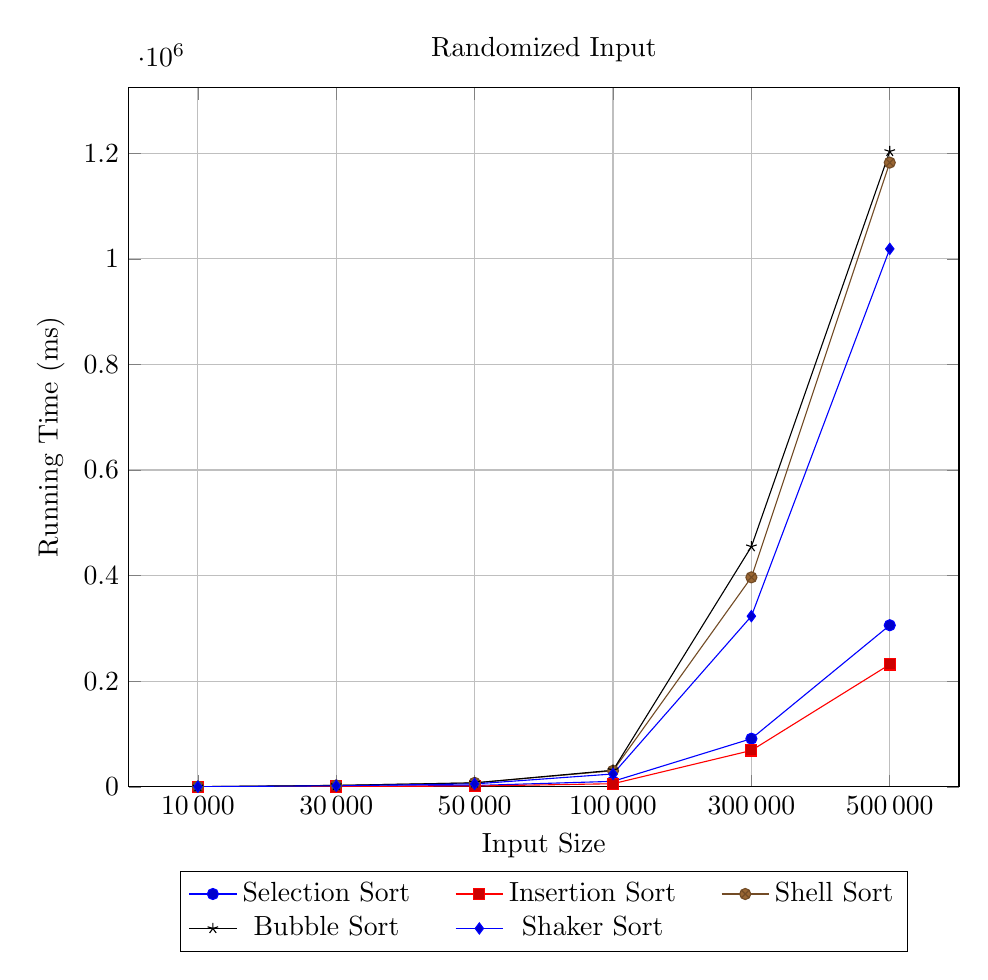
\begin{tikzpicture}
    \begin{axis}[
        width=\textwidth,
        title={Randomized Input},
        xlabel={Input Size},
        ylabel={Running Time (ms)},
        legend style={
            at={(0.5,-0.12)}, anchor=north, legend columns=3, 
            /tikz/every even column/.append style={column sep=0.5cm}
        },
        symbolic x coords={10\,000, 30\,000, 50\,000, 100\,000, 300\,000, 500\,000},
        xtick=data,
        ymin=0,
        grid=major,
    ]
    
    \addplot coordinates {(10\,000,110) (30\,000,870) (50\,000,2474) 
    (100\,000,10378) (300\,000,91156) (500\,000,306006)};
    \addlegendentry{Selection Sort}
    
    \addplot coordinates {(10\,000,58) (30\,000,504) (50\,000,1481) 
    (100\,000,5879) (300\,000,68865) (500\,000,231821)};
    \addlegendentry{Insertion Sort}
    
    \addplot coordinates {(10\,000,271) (30\,000,2692) (50\,000,7542) 
    (100\,000,30370) (300\,000,396729) (500\,000,1182221)};
    \addlegendentry{Shell Sort}
    
    \addplot coordinates {(10\,000,268) (30\,000,2639) (50\,000,7491) 
    (100\,000,31385) (300\,000,454882) (500\,000,1203413)};
    \addlegendentry{Bubble Sort}
    
    \addplot coordinates {(10\,000,219) (30\,000,1986) 
    (50\,000,5519) (100\,000,24340) (300\,000,323182) (500\,000,1018829)};
    \addlegendentry{Shaker Sort}
    
    \end{axis}
\end{tikzpicture}
\caption{Kết quả thực nghiệm với đầu vào có thứ tự ngẫu nhiên (Nhóm 1)}
\end{figure}

\begin{figure}[H]
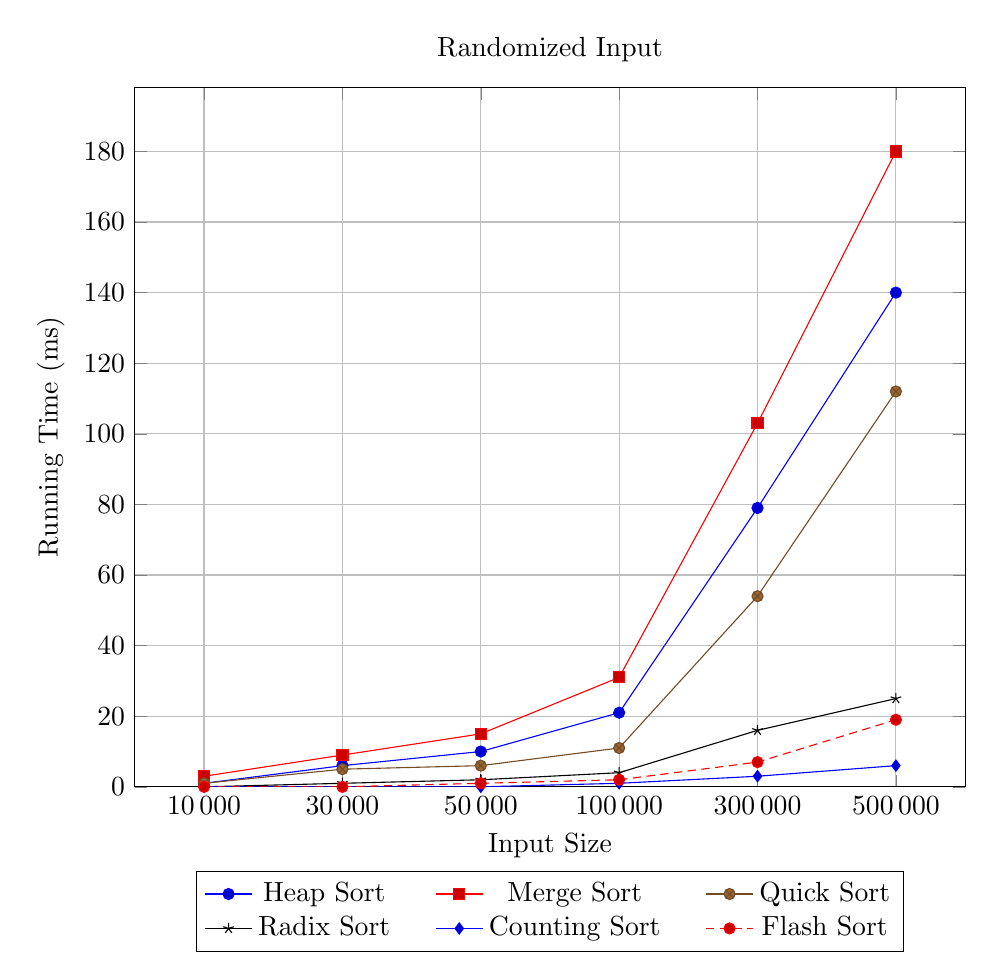
\begin{tikzpicture}
    \begin{axis}[
        width=\textwidth,
        title={Randomized Input},
        xlabel={Input Size},
        ylabel={Running Time (ms)},
        legend style={
            at={(0.5,-0.12)}, anchor=north, legend columns=3, 
            /tikz/every even column/.append style={column sep=0.5cm}
        },
        symbolic x coords={10\,000, 30\,000, 50\,000, 100\,000, 300\,000, 500\,000},
        xtick=data,
        ymin=0,
        grid=major,
    ]
    
    \addplot coordinates {(10\,000,1) (30\,000,6) (50\,000,10) 
    (100\,000,21) (300\,000,79) (500\,000,140)};
    \addlegendentry{Heap Sort}
    
    \addplot coordinates {(10\,000,3) (30\,000,9) (50\,000,15) 
    (100\,000,31) (300\,000,103) (500\,000,180)};
    \addlegendentry{Merge Sort}
    
    \addplot coordinates {(10\,000,1) (30\,000,5) (50\,000,6) 
    (100\,000,11) (300\,000,54) (500\,000,112)};
    \addlegendentry{Quick Sort}
    
    \addplot coordinates {(10\,000,0) (30\,000,1) (50\,000,2) 
    (100\,000,4) (300\,000,16) (500\,000,25)};
    \addlegendentry{Radix Sort}
    
    \addplot coordinates {(10\,000,0) (30\,000,0) (50\,000,0) 
    (100\,000,1) (300\,000,3) (500\,000,6)};
    \addlegendentry{Counting Sort}
    
    \addplot coordinates {(10\,000,0) (30\,000,0) (50\,000,1) 
    (100\,000,2) (300\,000,7) (500\,000,19)};
    \addlegendentry{Flash Sort}
    
    \end{axis}
\end{tikzpicture}
\caption{Kết quả thực nghiệm với đầu vào có thứ tự ngẫu nhiên (Nhóm 2)}
\end{figure}

\begin{itemize}[label=$\circ$]
    \item Thuật toán Bubble Sort có tốc độ chậm nhất với mọi kích thước 
    đầu vào, ngược lại Insertion Sort nhanh nhất trong nhóm thuật toán 
    có độ phức tạp là $O\left(n^2\right)$ cho dù số lượng phần tử có tăng 
    cao, thì thời gian thực thi vẫn không tăng quá nhiều. 
    \item Về nhóm thuật toán có độ phức tạp là $O\left(nlogn\right)$, 
    Merge Sort chậm đi rất nhiều khi kích thước đầu vào tăng lên do tiêu 
    tốn nhiều thời gian cho việc chia và trộn nhiều mảng con. Còn Quick 
    Sort mặc dù có tăng thời gian thực thi khi cỡ mẫu lớn hơn 100,000 
    nhưng vẫn nhanh nhất trong nhóm thuật toán này. 
    \item Cuối cùng là nhóm thuật toán có độ phức tạp là $O\left(n\right)$, 
    Counting Sort giữ vị trí thứ nhất nhưng bị hạn chế về kiểu dữ liệu, 
    như với số thực hoặc số nguyên lớn cần phải xử lý một cách khéo léo. 
    Mặc khác, Flash Sort có thể xử lý đa dạng kiểu dữ liệu và tốc độ cũng 
    đáng kể nhưng phụ thuộc vào sự phân phối của dữ liệu đầu vào và quá 
    trình cài đặt khá phức tạp.
\end{itemize}

$\bullet$ \textbf{Với đầu vào có thứ tự gần được sắp xếp}

\begin{figure}[H]
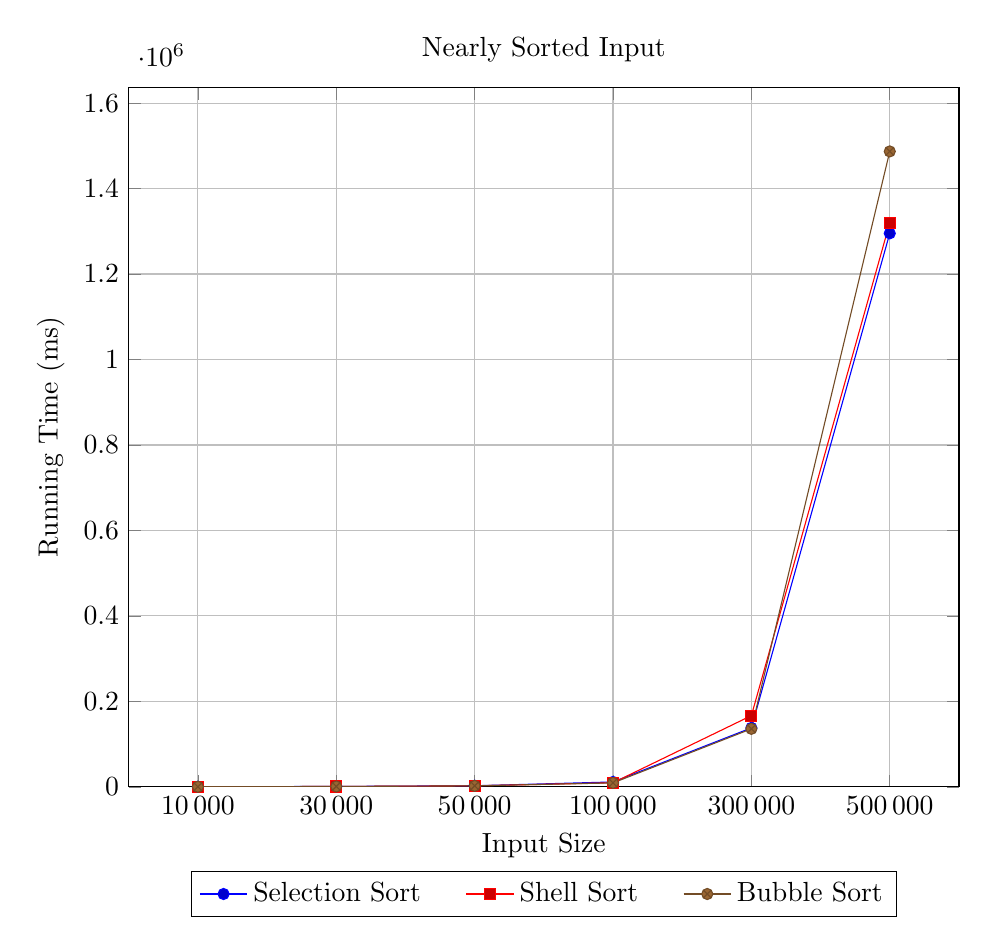
\begin{tikzpicture}
    \begin{axis}[
        width=\textwidth,
        title={Nearly Sorted Input},
        xlabel={Input Size},
        ylabel={Running Time (ms)},
        legend style={
            at={(0.5,-0.12)}, anchor=north, legend columns=3, 
            /tikz/every even column/.append style={column sep=0.5cm}
        },
        symbolic x coords={10\,000, 30\,000, 50\,000, 100\,000, 300\,000, 500\,000},
        xtick=data,
        ymin=0,
        grid=major,
    ]
    
    \addplot coordinates {(10\,000,106) (30\,000,868) (50\,000,2472) 
    (100\,000,11396) (300\,000,137957) (500\,000,1295243)};
    \addlegendentry{Selection Sort}
    
    \addplot coordinates {(10\,000,96) (30\,000,812) (50\,000,2290) 
    (100\,000,9538) (300\,000,166585) (500\,000,1319995)};
    \addlegendentry{Shell Sort}
    
    \addplot coordinates {(10\,000,94) (30\,000,828) (50\,000,2259) 
    (100\,000,9164) (300\,000,135698) (500\,000,1486996)};
    \addlegendentry{Bubble Sort}
    
    \end{axis}
\end{tikzpicture}
\caption{Kết quả thực nghiệm với đầu vào có thứ tự gần được sắp xếp (Nhóm 1)}
\end{figure}

\begin{figure}[H]
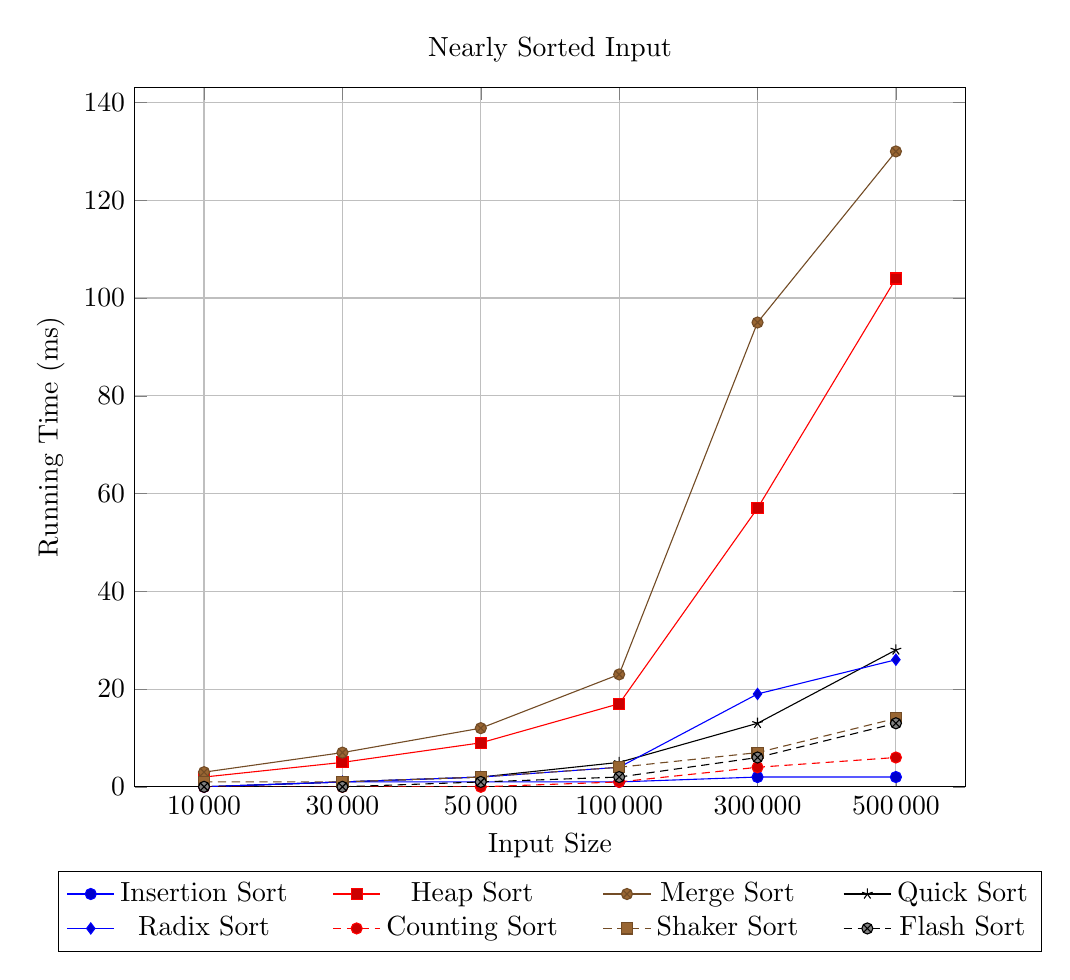
\begin{tikzpicture}
    \begin{axis}[
        width=\textwidth,
        title={Nearly Sorted Input},
        xlabel={Input Size},
        ylabel={Running Time (ms)},
        legend style={
            at={(0.5,-0.12)}, anchor=north, legend columns=4, 
            /tikz/every even column/.append style={column sep=0.5cm}
        },
        symbolic x coords={10\,000, 30\,000, 50\,000, 100\,000, 300\,000, 500\,000},
        xtick=data,
        ymin=0,
        grid=major,
    ]
    
    \addplot coordinates {(10\,000,0) (30\,000,1) (50\,000,1) 
    (100\,000,1) (300\,000,2) (500\,000,2)};
    \addlegendentry{Insertion Sort}
    
    \addplot coordinates {(10\,000,2) (30\,000,5) (50\,000,9) 
    (100\,000,17) (300\,000,57) (500\,000,104)};
    \addlegendentry{Heap Sort}
    
    \addplot coordinates {(10\,000,3) (30\,000,7) (50\,000,12) 
    (100\,000,23) (300\,000,95) (500\,000,130)};
    \addlegendentry{Merge Sort}
    
    \addplot coordinates {(10\,000,0) (30\,000,1) (50\,000,2) 
    (100\,000,5) (300\,000,13) (500\,000,28)};
    \addlegendentry{Quick Sort}
    
    \addplot coordinates {(10\,000,0) (30\,000,1) (50\,000,2) 
    (100\,000,4) (300\,000,19) (500\,000,26)};
    \addlegendentry{Radix Sort}
    
    \addplot coordinates {(10\,000,0) (30\,000,0) (50\,000,0) 
    (100\,000,1) (300\,000,4) (500\,000,6)};
    \addlegendentry{Counting Sort}
    
    \addplot coordinates {(10\,000,1) (30\,000,1) (50\,000,2) 
    (100\,000,4) (300\,000,7) (500\,000,14)};
    \addlegendentry{Shaker Sort}
    
    \addplot coordinates {(10\,000,0) (30\,000,0) (50\,000,1) 
    (100\,000,2) (300\,000,6) (500\,000,13)};
    \addlegendentry{Flash Sort}
    
    \end{axis}
\end{tikzpicture}
\caption{Kết quả thực nghiệm với đầu vào có thứ tự gần được sắp xếp (Nhóm 2)}
\end{figure}

\begin{itemize}[label=$\circ$]
    \item Các thuật toán như Selection Sort, Shell Sort, Bubble Sort, 
    Merge Sort và Heap Sort đều không có nhiều cải thiện. Ngược lại, 
    Shaker Sort, Insertion Sort và Quick Sort đã giảm đáng kể thời gian 
    thực thi xuống ngang bằng với nhóm thuật toán có độ phức tạp thời 
    gian là $O\left(n\right)$, thậm chí Insertion Sort còn giữ vị trí 
    nhanh nhất do chỉ cần đưa một vài phần tử nằm sai vị trí về đúng chỗ.
\end{itemize}

$\bullet$ \textbf{Với đầu vào có thứ tự đã được sắp xếp}

\begin{figure}[H]
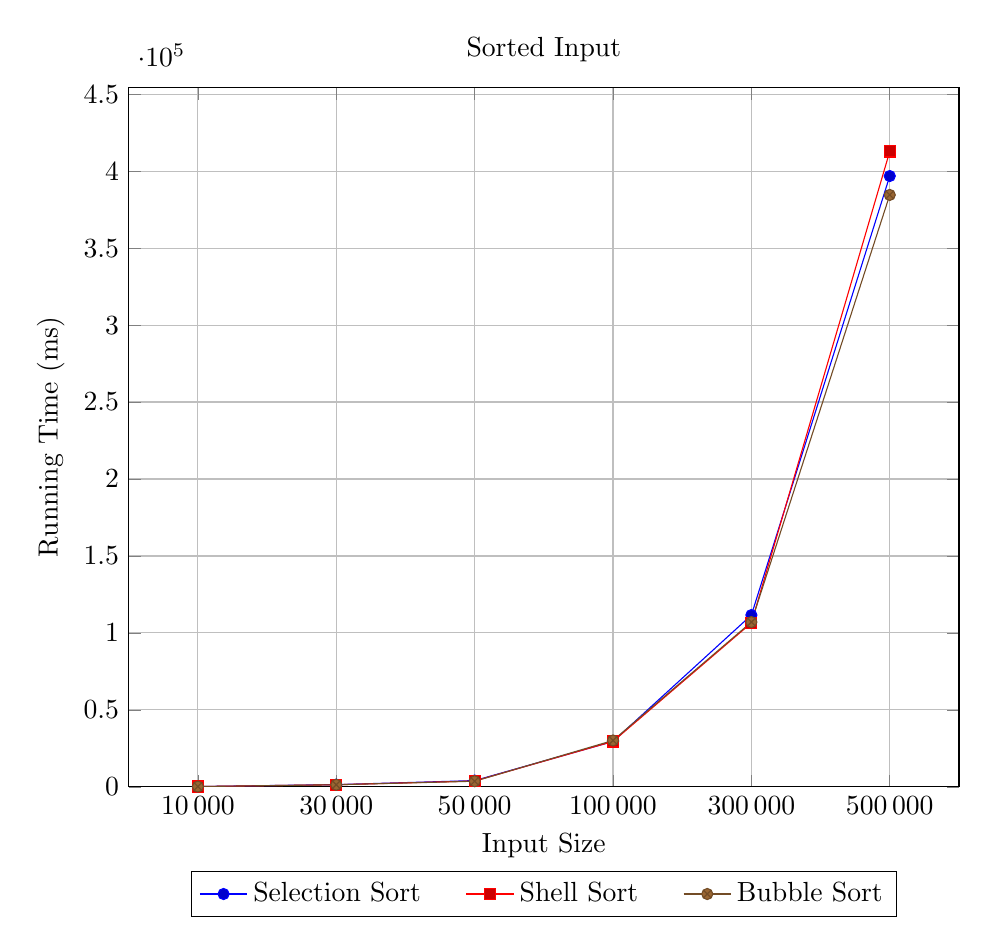
\begin{tikzpicture}
    \begin{axis}[
        width=\textwidth,
        title={Sorted Input},
        xlabel={Input Size},
        ylabel={Running Time (ms)},
        legend style={
            at={(0.5,-0.12)}, anchor=north, legend columns=3, 
            /tikz/every even column/.append style={column sep=0.5cm}
        },
        symbolic x coords={10\,000, 30\,000, 50\,000, 100\,000, 300\,000, 500\,000},
        xtick=data,
        ymin=0,
        grid=major,
    ]

    \addplot coordinates {(10\,000,182) (30\,000,1426) (50\,000,4059) 
    (100\,000,29478) (300\,000,111585) (500\,000,396841)};
    \addlegendentry{Selection Sort}
    
    \addplot coordinates {(10\,000,179) (30\,000,1349) (50\,000,3786) 
    (100\,000,29503) (300\,000,106498) (500\,000,412844)};
    \addlegendentry{Shell Sort}
    
    \addplot coordinates {(10\,000,180) (30\,000,1346) (50\,000,3636) 
    (100\,000,30120) (300\,000,107040) (500\,000,384574)};
    \addlegendentry{Bubble Sort}
    \end{axis}
\end{tikzpicture}
\caption{Kết quả thực nghiệm với đầu vào có thứ tự đã được sắp xếp (Nhóm 1)}
\end{figure}

\begin{figure}[H]
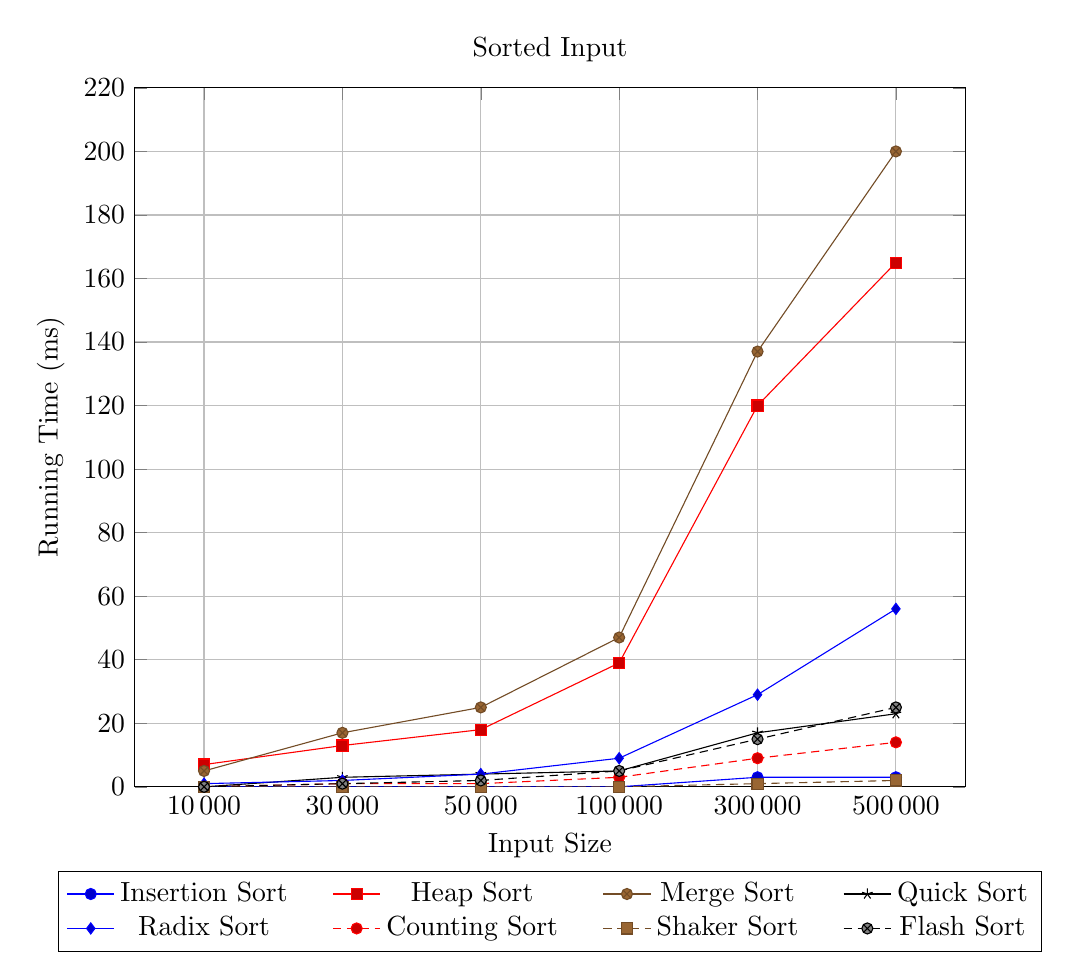
\begin{tikzpicture}
    \begin{axis}[
        width=\textwidth,
        title={Sorted Input},
        xlabel={Input Size},
        ylabel={Running Time (ms)},
        legend style={
            at={(0.5,-0.12)}, anchor=north, legend columns=4, 
            /tikz/every even column/.append style={column sep=0.5cm}
        },
        symbolic x coords={10\,000, 30\,000, 50\,000, 100\,000, 300\,000, 500\,000},
        xtick=data,
        ymin=0,
        grid=major,
    ]
    
    \addplot coordinates {(10\,000,0) (30\,000,0) (50\,000,0) 
    (100\,000,0) (300\,000,3) (500\,000,3)};
    \addlegendentry{Insertion Sort}
    
    \addplot coordinates {(10\,000,7) (30\,000,13) (50\,000,18) 
    (100\,000,39) (300\,000,120) (500\,000,165)};
    \addlegendentry{Heap Sort}
    
    \addplot coordinates {(10\,000,5) (30\,000,17) (50\,000,25) 
    (100\,000,47) (300\,000,137) (500\,000,200)};
    \addlegendentry{Merge Sort}
    
    \addplot coordinates {(10\,000,0) (30\,000,3) (50\,000,4) 
    (100\,000,5) (300\,000,17) (500\,000,23)};
    \addlegendentry{Quick Sort}
    
    \addplot coordinates {(10\,000,1) (30\,000,2) (50\,000,4) 
    (100\,000,9) (300\,000,29) (500\,000,56)};
    \addlegendentry{Radix Sort}
    
    \addplot coordinates {(10\,000,0) (30\,000,1) (50\,000,1) 
    (100\,000,3) (300\,000,9) (500\,000,14)};
    \addlegendentry{Counting Sort}
    
    \addplot coordinates {(10\,000,0) (30\,000,0) (50\,000,0) 
    (100\,000,0) (300\,000,1) (500\,000,2)};
    \addlegendentry{Shaker Sort}
    
    \addplot coordinates {(10\,000,0) (30\,000,1) (50\,000,2) 
    (100\,000,5) (300\,000,15) (500\,000,25)};
    \addlegendentry{Flash Sort}
    
    \end{axis}
\end{tikzpicture}
\caption{Kết quả thực nghiệm với đầu vào có thứ tự đã được sắp xếp (Nhóm 2)}
\end{figure}

\begin{itemize}[label=$\circ$]
    \item Trong nhóm thuật toán có độ phức tạp $O\left(n^2\right)$ thì 
    Insertion Sort và Shaker Sort có tốc độ rất nhanh và hầu như là không 
    tốn thời gian với 100,000 phần tử. Ngược lại, 2 thuật toán còn lại 
    là Select Sort và Bubble Sort thì lại tốn khá nhiều thời gian và có 
    thời gian chạy không chênh lệch nhiều so với nhau.
    \item Trong nhóm thuật toán có độ phức tạp $O\left(n\log{n}\right)$ 
    thì Shell Sort lại dường như tốn rất nhiều thời gian tương đương với 
    một số thuật toán thuộc $O\left(n^2\right)$, còn Quick Sort là thuật 
    toán có thời gian chạy nhanh nhất, Heap Sort thì nhanh hơn Merge Sort 
    một chút.
    \item Trong nhóm thuật toán có độ phức tạp $O\left(n\right)$ thì 
    Counting Sort vẫn có thời gian chạy nhanh nhất, còn Radix Sort thì 
    có thời gian chạy chậm nhất trong nhóm thuật toán này.
\end{itemize}

$\bullet$ \textbf{Với đầu vào có thứ tự được sắp xếp ngược}

\begin{figure}[H]
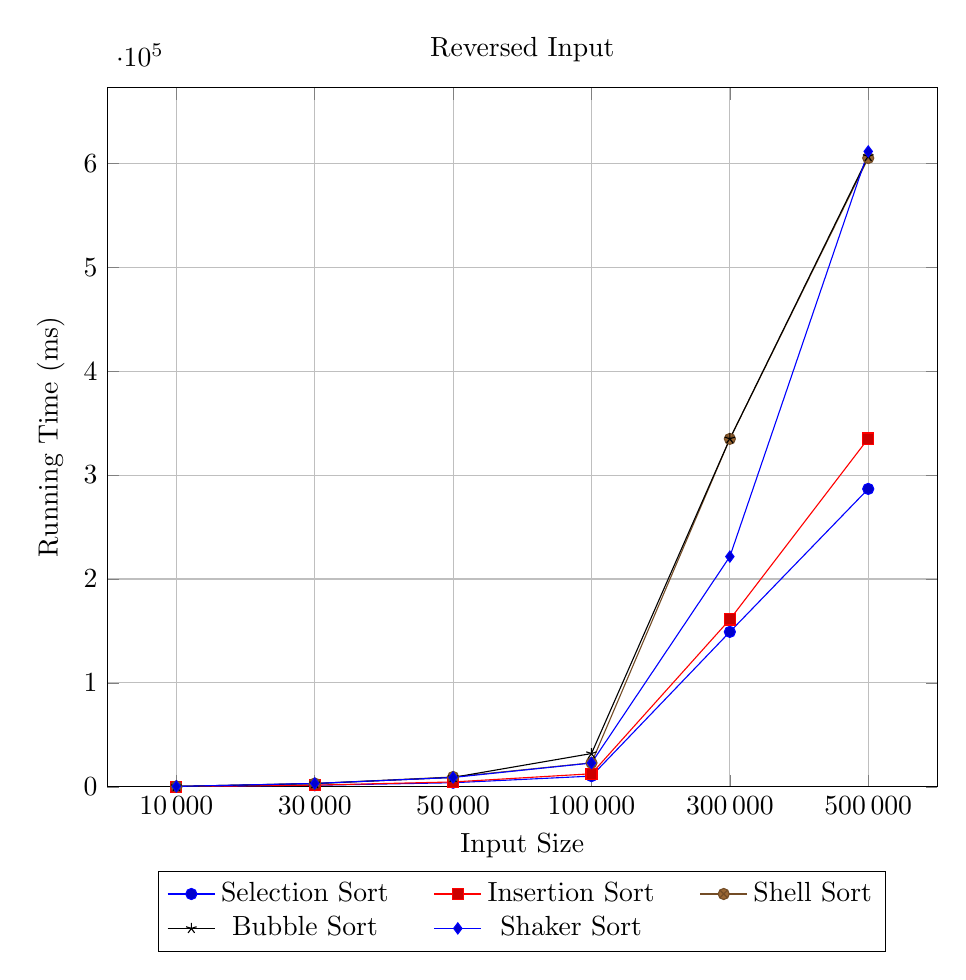
\begin{tikzpicture}
    \begin{axis}[
        width=\textwidth,
        title={Reversed Input},
        xlabel={Input Size},
        ylabel={Running Time (ms)},
        legend style={
            at={(0.5,-0.12)}, anchor=north, legend columns=3, 
            /tikz/every even column/.append style={column sep=0.5cm}
        },
        symbolic x coords={10\,000, 30\,000, 50\,000, 100\,000, 300\,000, 500\,000},
        xtick=data,
        ymin=0,
        grid=major,
    ]
    
    \addplot coordinates {(10\,000,175) (30\,000,1477) (50\,000,3924) 
    (100\,000,10289) (300\,000,149091) (500\,000,286666)};
    \addlegendentry{Selection Sort}
    
    \addplot coordinates {(10\,000,202) (30\,000,1630) (50\,000,4686) 
    (100\,000,12560) (300\,000,161038) (500\,000,335113)};
    \addlegendentry{Insertion Sort}
    
    \addplot coordinates {(10\,000,383) (30\,000,3158) (50\,000,9485) 
    (100\,000,23060) (300\,000,334815) (500\,000,605040)};
    \addlegendentry{Shell Sort}
    
    \addplot coordinates {(10\,000,373) (30\,000,3116) (50\,000,9043) 
    (100\,000,32013) (300\,000,334914) (500\,000,606656)};
    \addlegendentry{Bubble Sort}
    
    \addplot coordinates {(10\,000,385) (30\,000,3255) (50\,000,9005) 
    (100\,000,22892) (300\,000,221549) (500\,000,611441)};
    \addlegendentry{Shaker Sort}
    
    \end{axis}
\end{tikzpicture}
\caption{Kết quả thực nghiệm với đầu vào có thứ tự được sắp xếp ngược (Nhóm 1)}
\end{figure}

\begin{figure}[H]
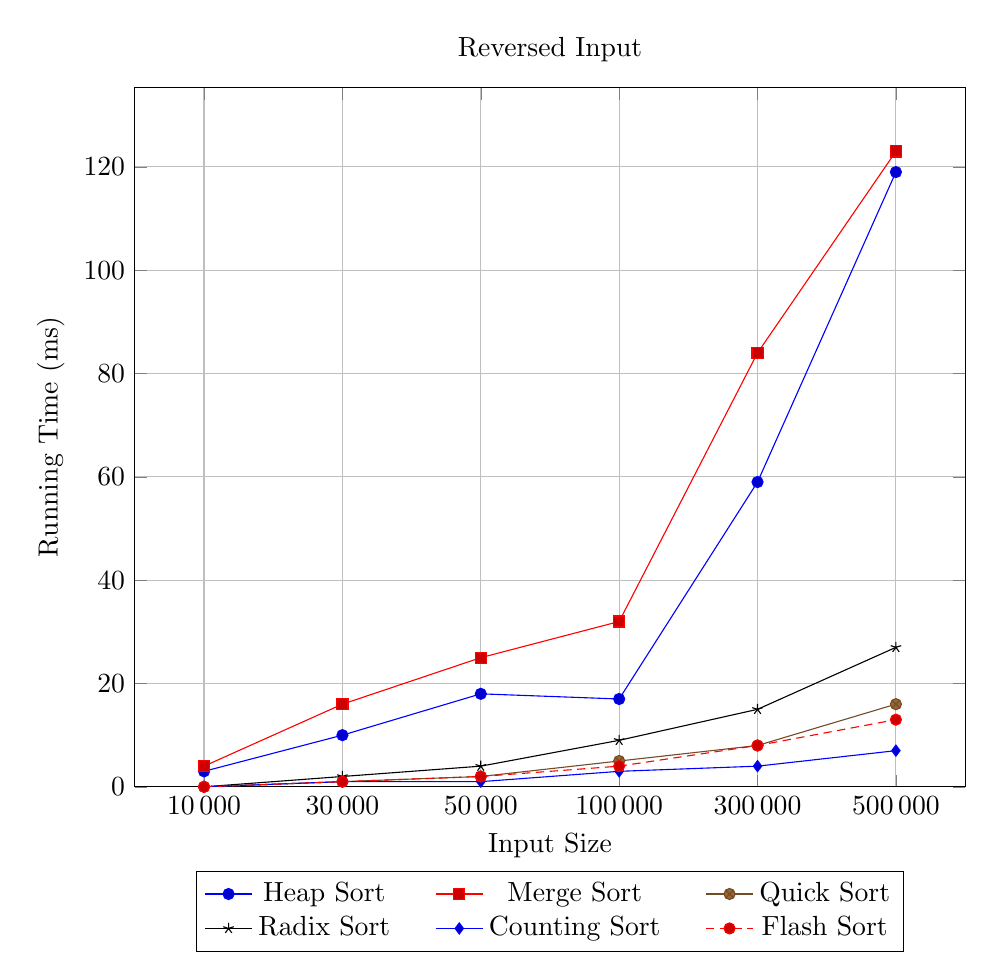
\begin{tikzpicture}
    \begin{axis}[
        width=\textwidth,
        title={Reversed Input},
        xlabel={Input Size},
        ylabel={Running Time (ms)},
        legend style={
            at={(0.5,-0.12)}, anchor=north, legend columns=3, 
            /tikz/every even column/.append style={column sep=0.5cm}
        },
        symbolic x coords={10\,000, 30\,000, 50\,000, 100\,000, 300\,000, 500\,000},
        xtick=data,
        ymin=0,
        grid=major,
    ]
    
    \addplot coordinates {(10\,000,3) (30\,000,10) (50\,000,18) 
    (100\,000,17) (300\,000,59) (500\,000,119)};
    \addlegendentry{Heap Sort}
    
    \addplot coordinates {(10\,000,4) (30\,000,16) (50\,000,25) 
    (100\,000,32) (300\,000,84) (500\,000,123)};
    \addlegendentry{Merge Sort}
    
    \addplot coordinates {(10\,000,0) (30\,000,1) (50\,000,2) 
    (100\,000,5) (300\,000,8) (500\,000,16)};
    \addlegendentry{Quick Sort}
    
    \addplot coordinates {(10\,000,0) (30\,000,2) (50\,000,4) 
    (100\,000,9) (300\,000,15) (500\,000,27)};
    \addlegendentry{Radix Sort}
    
    \addplot coordinates {(10\,000,0) (30\,000,1) (50\,000,1) 
    (100\,000,3) (300\,000,4) (500\,000,7)};
    \addlegendentry{Counting Sort}
    
    \addplot coordinates {(10\,000,0) (30\,000,1) (50\,000,2) 
    (100\,000,4) (300\,000,8) (500\,000,13)};
    \addlegendentry{Flash Sort}
    
    \end{axis}
\end{tikzpicture}
\caption{Kết quả thực nghiệm với đầu vào có thứ tự được sắp xếp ngược (Nhóm 2)}
\end{figure}

\begin{itemize}[label=$\circ$]
    \item Các thuật toán như Selection Sort, Shell Sort, Bubble Sort, 
    Merge Sort, và Heap Sort đều thể hiện thời gian thực thi cao, đặc 
    biệt là nhóm các thuật toán có độ phức tạp thời gian trung bình là 
    $O\left(n^2\right)$. Những thuật toán như Bubble Sort và Shaker Sort 
    trở nên chậm đáng kể do cần nhiều phép hoán đổi, trong khi Selection 
    Sort duy trì hiệu suất ổn định nhưng vẫn kém hiệu quả vì phải duyệt 
    toàn bộ danh sách để tìm giá trị nhỏ nhất.
    \item Ngược lại, nhóm thuật toán có độ phức tạp trung bình là 
    $O\left(n\log{n}\right)$ như Quick Sort, Merge Sort và Heap Sort thể 
    hiện hiệu suất vượt trội hơn, với Merge Sort và Heap Sort ổn định hơn 
    so với Quick Sort do đặc thù phân chia dữ liệu của chúng.
    \item Đặc biệt, các thuật toán có độ phức tạp $O\left(n\right)$ như 
    Counting Sort và Flash Sort cho thấy thời gian thực thi thấp nhất 
    trong các biểu đồ, chứng minh tính vượt trội khi xử lý các dữ liệu 
    lớn ngay cả trong trường hợp xấu nhất.
\end{itemize}

\subsubsection{Về số phép so sánh}

$\bullet$ \textbf{Với đầu vào có thứ tự ngẫu nhiên}

\begin{figure}[H]
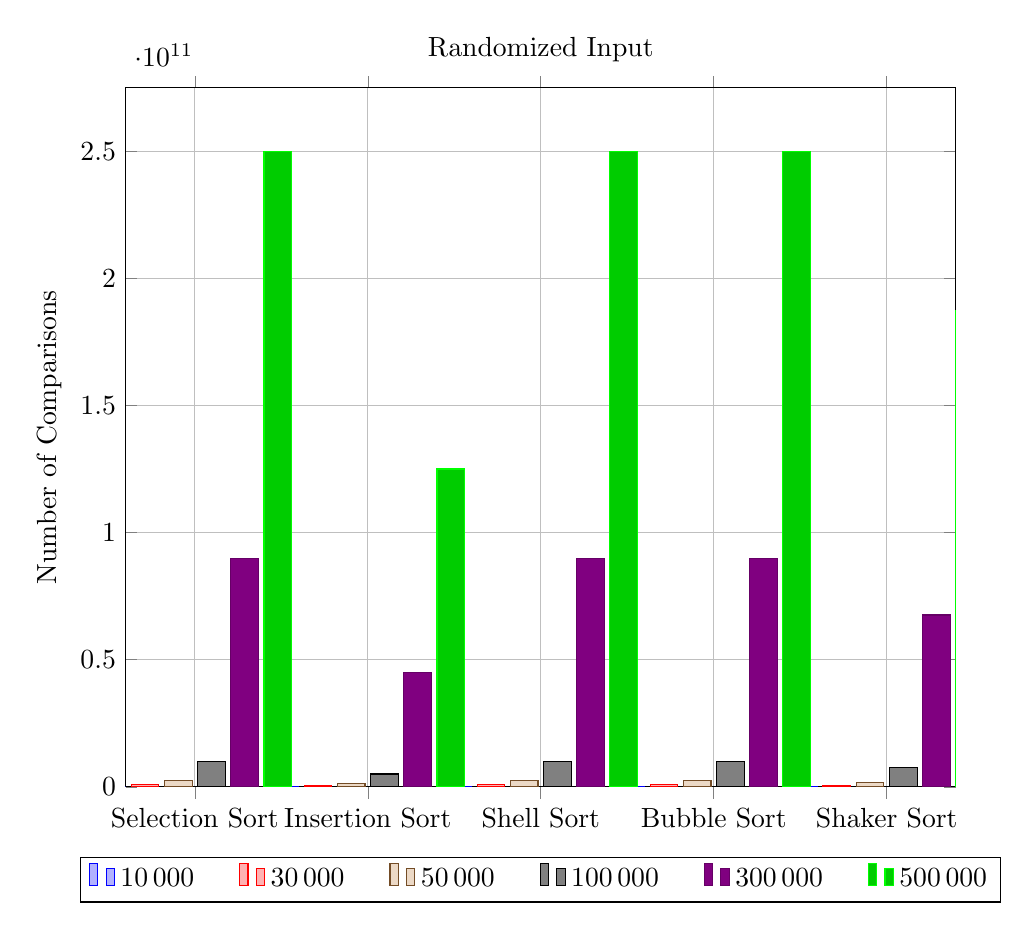
\begin{tikzpicture}
    \begin{axis}[
        width=\textwidth,
        title={Randomized Input},
        ybar,
        ymin=0,
        grid=major,
        legend style={
            at={(0.5,-0.1)}, anchor=north, legend columns=-1,
            /tikz/every even column/.append style={column sep=0.5cm}
        },
        ylabel={Number of Comparisons},
        symbolic x coords={
            Selection Sort, Insertion Sort, Shell Sort, Bubble Sort, 
            Shaker Sort
        },
        xtick=data,
    ]
    \addplot coordinates {(Selection Sort,100009999) 
        (Insertion Sort,49852722) (Shell Sort,100009999) 
        (Bubble Sort,100009999) (Shaker Sort,75877345)};
    \addplot coordinates {(Selection Sort,900029999) 
        (Insertion Sort,450424387) (Shell Sort,900029999) 
        (Bubble Sort,900029999) (Shaker Sort,678034901)};
    \addplot coordinates {(Selection Sort,2500049999) 
        (Insertion Sort,1244875082) (Shell Sort,2500049999) 
        (Bubble Sort,2500049999) (Shaker Sort,1868558231)};
    \addplot coordinates {(Selection Sort,10000099999) 
        (Insertion Sort,5026592949) (Shell Sort,10000099999) 
        (Bubble Sort,10000099999) (Shaker Sort,7519014091)};
    \addplot coordinates {(Selection Sort,90000299999) 
        (Insertion Sort,44937080911) (Shell Sort,90000299999) 
        (Bubble Sort,90000299999) (Shaker Sort,67598742089)};
    \addplot coordinates {(Selection Sort,250000499999) 
        (Insertion Sort,125044404674) (Shell Sort,250000499999) 
        (Bubble Sort,250000499999) (Shaker Sort,187569730819)};
        \legend{10\,000, 30\,000, 50\,000, 100\,000, 300\,000, 500\,000}
    \end{axis}
\end{tikzpicture}
\caption{Kết quả thực nghiệm với đầu vào có thứ tự ngẫu nhiên (Nhóm 1)}
\end{figure}

\begin{figure}[H]
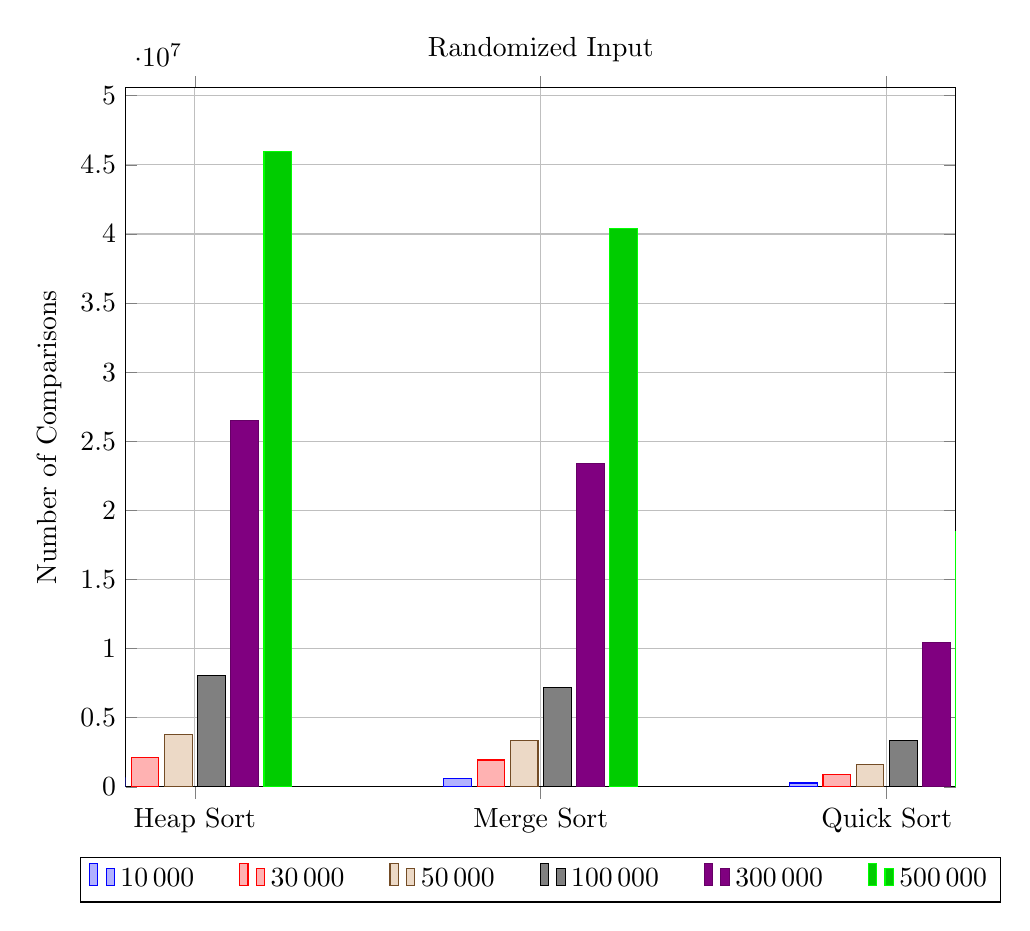
\begin{tikzpicture}
    \begin{axis}[
        width=\textwidth,
        title={Randomized Input},
        ybar,
        ymin=0,
        grid=major,
        legend style={
            at={(0.5,-0.1)}, anchor=north, legend columns=-1,
            /tikz/every even column/.append style={column sep=0.5cm}
        },
        ylabel={Number of Comparisons},
        symbolic x coords={Heap Sort, Merge Sort, Quick Sort},
        xtick=data,
    ]
    \addplot coordinates {(Heap Sort,638425) 
        (Merge Sort,583832) (Quick Sort,276045)};
    \addplot coordinates {(Heap Sort,2150786) 
        (Merge Sort,1937240) (Quick Sort,916849)};
    \addplot coordinates {(Heap Sort,3771772) 
        (Merge Sort,3383319) (Quick Sort,1636700)};
    \addplot coordinates {(Heap Sort,8044992) 
        (Merge Sort,7166010) (Quick Sort,3341712)};
    \addplot coordinates {(Heap Sort,26487787) 
        (Merge Sort,23383601) (Quick Sort,10434674)};
    \addplot coordinates {(Heap Sort,45972193) 
        (Merge Sort,40383061) (Quick Sort,18476753)};
    \legend{10\,000, 30\,000, 50\,000, 100\,000, 300\,000, 500\,000}
    \end{axis}
\end{tikzpicture}
\caption{Kết quả thực nghiệm với đầu vào có thứ tự ngẫu nhiên (Nhóm 2)}
\end{figure}

\begin{figure}[H]
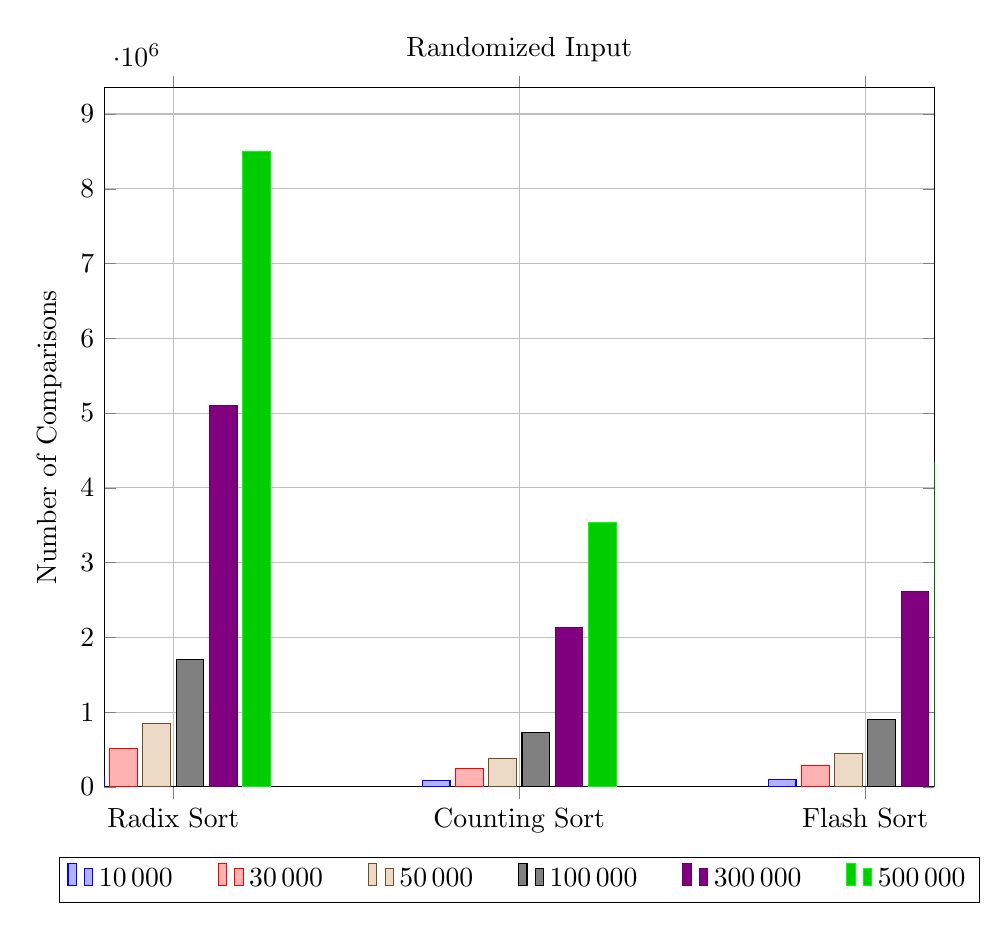
\begin{tikzpicture}
    \begin{axis}[
        width=\textwidth,
        title={Randomized Input},
        ybar,
        ymin=0,
        grid=major,
        legend style={
            at={(0.5,-0.1)}, anchor=north, legend columns=-1,
            /tikz/every even column/.append style={column sep=0.5cm}
        },
        ylabel={Number of Comparisons},
        symbolic x coords={Radix Sort, Counting Sort, Flash Sort},
        xtick=data,
    ]
    \addplot coordinates {(Radix Sort,140056) 
        (Counting Sort,80000) (Flash Sort,97658)};
    \addplot coordinates {(Radix Sort,510070) 
        (Counting Sort,240000) (Flash Sort,285201)};
    \addplot coordinates {(Radix Sort,850070) 
        (Counting Sort,382769) (Flash Sort,451390)};
    \addplot coordinates {(Radix Sort,1700070) 
        (Counting Sort,732769) (Flash Sort,905677)};
    \addplot coordinates {(Radix Sort,5100070) 
        (Counting Sort,2132769) (Flash Sort,2611012)};
    \addplot coordinates {(Radix Sort,8500070) 
        (Counting Sort,3532769) (Flash Sort,4335083)};
    \legend{10\,000, 30\,000, 50\,000, 100\,000, 300\,000, 500\,000}
    \end{axis}
\end{tikzpicture}
\caption{Kết quả thực nghiệm với đầu vào có thứ tự ngẫu nhiên (Nhóm 3)}
\end{figure}

\begin{itemize}[label=$\circ$]
    \item Có thể nhận xét rằng số phép so sánh giữa các thuật toán sắp 
    xếp thay đổi đáng kể tùy thuộc vào độ phức tạp về thời gian của từng 
    thuật toán. Nhóm các thuật toán có số phép so sánh lớn nhất bao gồm 
    Selection Sort, Insertion Sort, Shell Sort, Bubble Sort và Shaker 
    Sort do có độ phức tạp $O\left(n^2\right)$. Trong đó, cả 3 thuật toán 
    gồm Selection Sort, Shell Sort, Bubble Sort đều có số phép so sánh 
    bằng nhau và lớn nhất so với 8 thuật toán còn lại. Điều này dẫn đến 
    số phép so sánh tăng nhanh khi kích thước mảng lớn, đặc biệt là ở các 
    mảng kích thước 300000 và 500000, với cột biểu đồ vượt trội hơn hẳn 
    so với các thuật toán khác.
	\item Trong khi đó, nhóm thuật toán có hiệu suất trung bình như Heap 
    Sort, Merge Sort, và Quick Sort hoạt động hiệu quả hơn nhờ độ phức 
    tạp $O\left(n\log{n}\right)$. Quick Sort có số phép so sánh thấp hơn 
    so với Heap Sort và Merge Sort, cho thấy ưu thế rõ rệt khi xử lý trên 
    mảng ngẫu nhiên.
	\item Cuối cùng, nhóm thuật toán có số phép so sánh thấp nhất bao 
    gồm Radix Sort, Counting Sort, và Flash Sort, nhờ đặc điểm không dựa 
    trên các phép so sánh với độ phức tạp gần như là $O\left(n\right)$. 
    Counting Sort đặc biệt nổi bật với số phép so sánh thấp nhất trong 
    nhóm này và thấp nhất trong 11 thuật toán.
\end{itemize}

$\bullet$ \textbf{Với đầu vào có thứ tự gần được sắp xếp}

\begin{figure}[H]
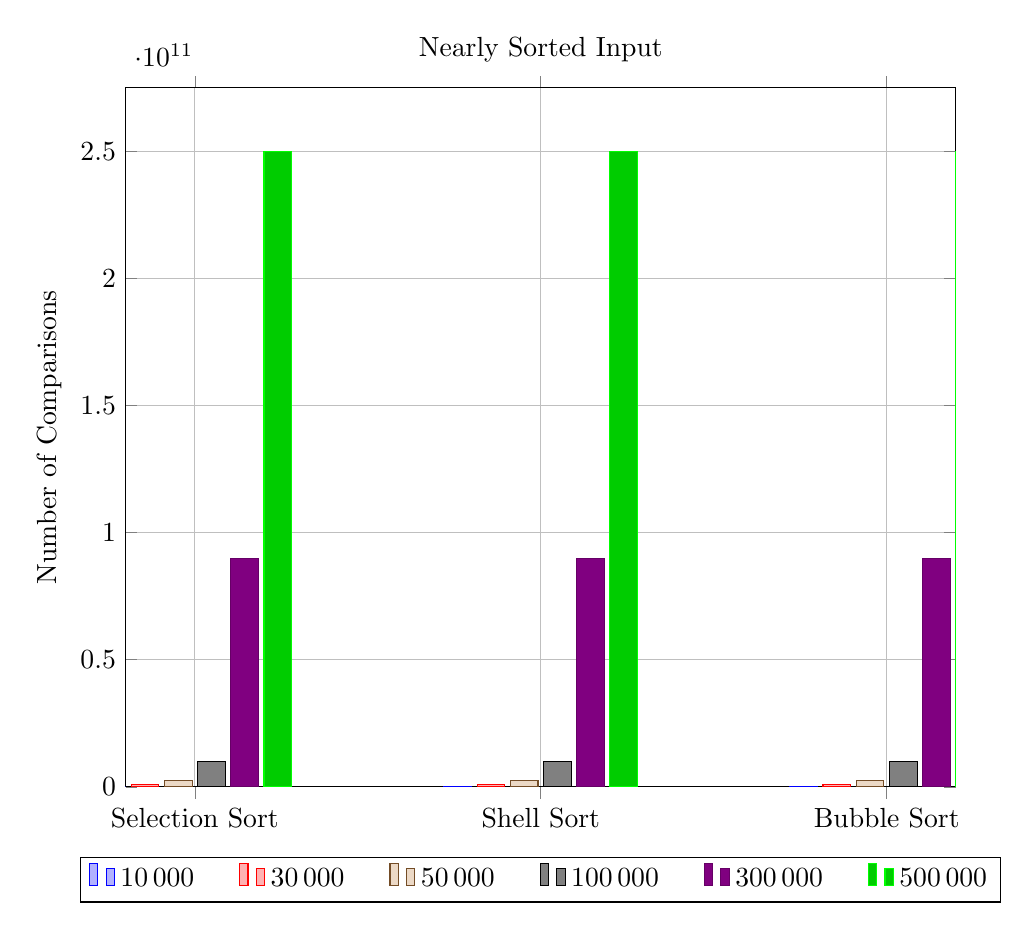
\begin{tikzpicture}
    \begin{axis}[
        width=\textwidth,
        title={Nearly Sorted Input},
        ybar,
        ymin=0,
        grid=major,
        legend style={
            at={(0.5,-0.1)}, anchor=north, legend columns=-1,
            /tikz/every even column/.append style={column sep=0.5cm}
        },
        ylabel={Number of Comparisons},
        symbolic x coords={Selection Sort, Shell Sort, Bubble Sort},
        xtick=data,
    ]
    \addplot coordinates {(Selection Sort,100009999) 
        (Shell Sort,100009999) (Bubble Sort,100009999)};
    \addplot coordinates {(Selection Sort,900029999) 
        (Shell Sort,900029999) (Bubble Sort,900029999)};
    \addplot coordinates {(Selection Sort,2500049999) 
        (Shell Sort,2500049999) (Bubble Sort,2500049999)};
    \addplot coordinates {(Selection Sort,10000099999) 
        (Shell Sort,10000099999) (Bubble Sort,10000099999)};
    \addplot coordinates {(Selection Sort,90000299999) 
        (Shell Sort,90000299999) (Bubble Sort,90000299999)};
    \addplot coordinates {(Selection Sort,250000499999) 
        (Shell Sort,250000499999) (Bubble Sort,250000499999)};
    \legend{10\,000, 30\,000, 50\,000, 100\,000, 300\,000, 500\,000}
    \end{axis}
\end{tikzpicture}
\caption{Kết quả thực nghiệm với đầu vào có thứ tự gần được sắp xếp (Nhóm 1)}
\end{figure}

\begin{figure}[H]
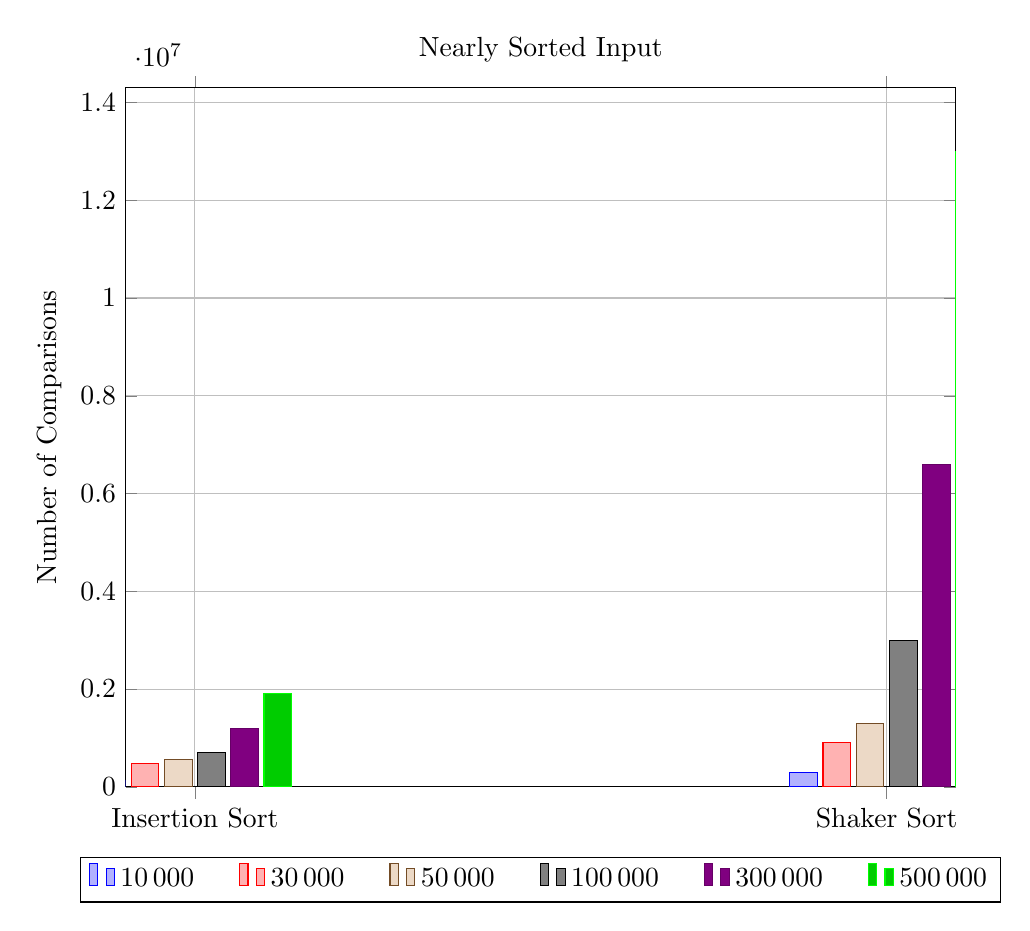
\begin{tikzpicture}
    \begin{axis}[
        width=\textwidth,
        title={Nearly Sorted Input},
        ybar,
        ymin=0,
        grid=major,
        legend style={
            at={(0.5,-0.1)}, anchor=north, legend columns=-1,
            /tikz/every even column/.append style={column sep=0.5cm}
        },
        ylabel={Number of Comparisons},
        symbolic x coords={Insertion Sort, Shaker Sort},
        xtick=data,
    ]
    \addplot coordinates {(Insertion Sort,129726) 
        (Shaker Sort,299791)};
    \addplot coordinates {(Insertion Sort,486366) 
        (Shaker Sort,899791)};
    \addplot coordinates {(Insertion Sort,560354) 
        (Shaker Sort,1299845)};
    \addplot coordinates {(Insertion Sort,706102) 
        (Shaker Sort,2999791)};
    \addplot coordinates {(Insertion Sort,1188582) 
        (Shaker Sort,6599891)};
    \addplot coordinates {(Insertion Sort,1905186) 
        (Shaker Sort,12999845)};
    \legend{10\,000, 30\,000, 50\,000, 100\,000, 300\,000, 500\,000}
    \end{axis}
\end{tikzpicture}
\caption{Kết quả thực nghiệm với đầu vào có thứ tự gần được sắp xếp (Nhóm 2)}
\end{figure}

\begin{figure}[H]
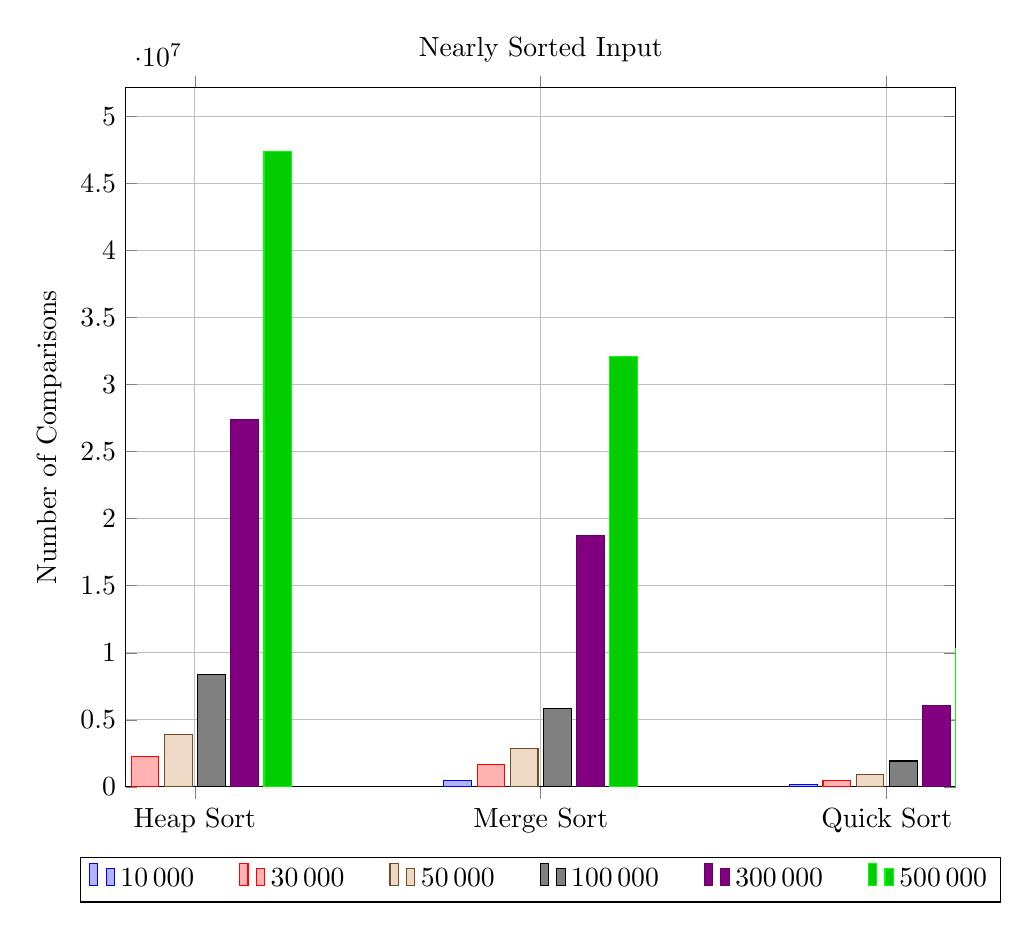
\begin{tikzpicture}
    \begin{axis}[
        width=\textwidth,
        title={Nearly Sorted Input},
        ybar,
        ymin=0,
        grid=major,
        legend style={
            at={(0.5,-0.1)}, anchor=north, legend columns=-1,
            /tikz/every even column/.append style={column sep=0.5cm}
        },
        ylabel={Number of Comparisons},
        symbolic x coords={Heap Sort, Merge Sort, Quick Sort},
        xtick=data,
    ]
    \addplot coordinates {(Heap Sort,669904) 
        (Merge Sort,503802) (Quick Sort,154995)};
    \addplot coordinates {(Heap Sort,2236774) 
        (Merge Sort,1637853) (Quick Sort,501973)};
    \addplot coordinates {(Heap Sort,3925280) 
        (Merge Sort,2845326) (Quick Sort,913890)};
    \addplot coordinates {(Heap Sort,8364715) 
        (Merge Sort,5851166) (Quick Sort,1927723)};
    \addplot coordinates {(Heap Sort,27413296) 
        (Merge Sort,18733795) (Quick Sort,6058264)};
    \addplot coordinates {(Heap Sort,47405047) 
        (Merge Sort,32137705) (Quick Sort,10310769)};
    \legend{10\,000, 30\,000, 50\,000, 100\,000, 300\,000, 500\,000}
    \end{axis}
\end{tikzpicture}
\caption{Kết quả thực nghiệm với đầu vào có thứ tự gần được sắp xếp (Nhóm 3)}
\end{figure}

\begin{figure}[H]
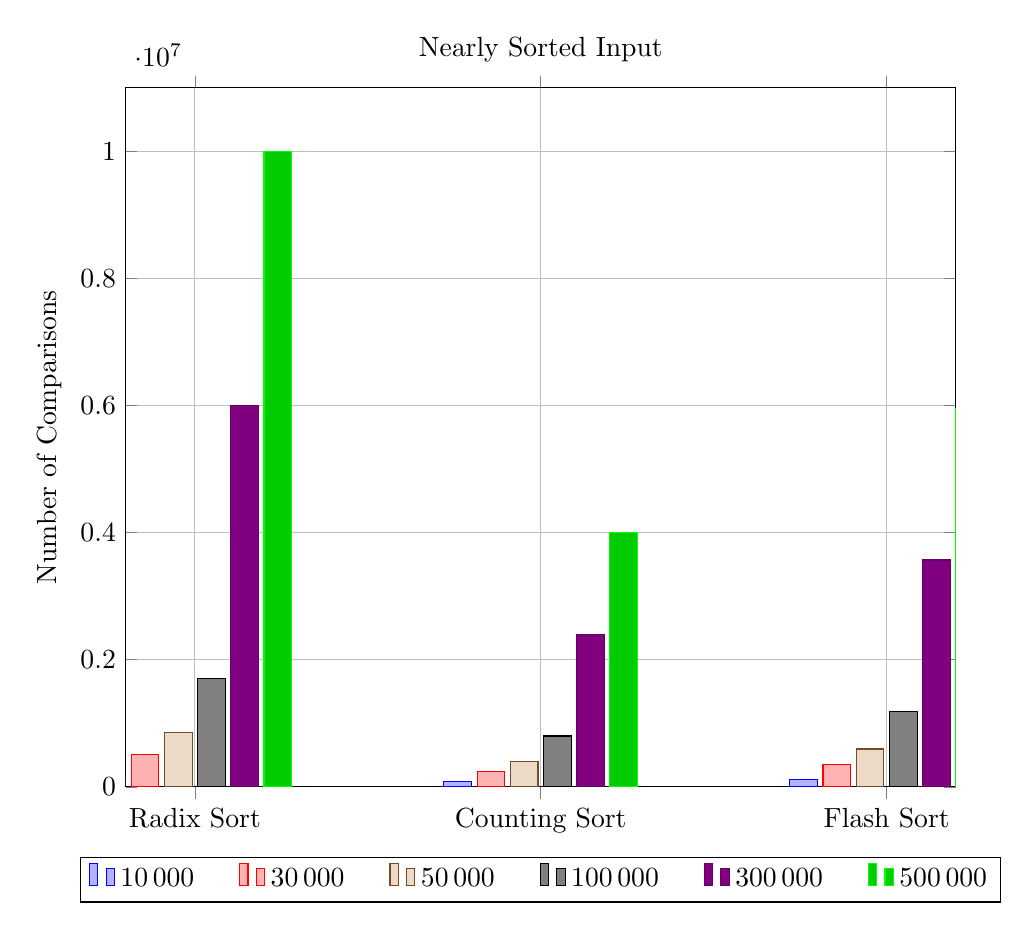
\begin{tikzpicture}
    \begin{axis}[
        width=\textwidth,
        title={Nearly Sorted Input},
        ybar,
        ymin=0,
        grid=major,
        legend style={
            at={(0.5,-0.1)}, anchor=north, legend columns=-1,
            /tikz/every even column/.append style={column sep=0.5cm}
        },
        ylabel={Number of Comparisons},
        symbolic x coords={Radix Sort, Counting Sort, Flash Sort},
        xtick=data,
    ]
    \addplot coordinates {(Radix Sort,140056) 
        (Counting Sort,80001) (Flash Sort,118969)};
    \addplot coordinates {(Radix Sort,510070) 
        (Counting Sort,240001) (Flash Sort,356969)};
    \addplot coordinates {(Radix Sort,850070) 
        (Counting Sort,400001) (Flash Sort,594969)};
    \addplot coordinates {(Radix Sort,1700070) 
        (Counting Sort,800001) (Flash Sort,1189967)};
    \addplot coordinates {(Radix Sort,6000084) 
        (Counting Sort,2400001) (Flash Sort,3569970)};
    \addplot coordinates {(Radix Sort,10000084) 
        (Counting Sort,4000001) (Flash Sort,5949970)};
    \legend{10\,000, 30\,000, 50\,000, 100\,000, 300\,000, 500\,000}
    \end{axis}
\end{tikzpicture}
\caption{Kết quả thực nghiệm với đầu vào có thứ tự gần được sắp xếp (Nhóm 4)}
\end{figure}

\begin{itemize}[label=$\circ$]
    \item Có thể nhận xét rằng số phép so sánh giữa các thuật toán sắp 
    xếp thay đổi đáng kể tùy thuộc vào độ phức tạp về thời gian và khả 
    năng tối ưu hóa đối với mảng đã có trật tự. Nhóm các thuật toán có 
    số phép so sánh lớn nhất bao gồm Selection Sort, Shell Sort, và 
    Bubble Sort do có độ phức tạp $O\left(n^2\right)$ và không tận dụng 
    được tính chất mảng gần như đã sắp xếp. Trong đó, cả ba thuật toán 
    này đều có số phép so sánh cao nhất, đặc biệt khi kích thước mảng 
    tăng lên 300000 và 500000, với cột biểu đồ vượt trội so với các 
    thuật toán khác. Insertion Sort, nhờ khả năng tối ưu hóa tốt cho 
    các mảng đã gần sắp xếp, thực hiện ít phép so sánh hơn đáng kể, 
    trong khi Shaker Sort (một biến thể của Bubble Sort) cũng cho thấy 
    hiệu năng cải thiện nhưng vẫn kém hiệu quả hơn Insertion Sort. 
	\item Đối với các thuật toán có độ phức tạp là $O\left(n\log{n}\right)$ 
    về thời gian, Heap Sort thực hiện nhiều phép so sánh hơn so với Merge 
    Sort và Quick Sort. Trong đó, Quick Sort tỏ ra vượt trội hơn Merge 
    Sort nhờ khả năng tận dụng tốt tính chất của mảng gần như được sắp xếp. 
	\item Cuối cùng, nhóm thuật toán có số phép so sánh thấp nhất bao 
    gồm Radix Sort, Counting Sort và Flash Sort, nhờ đặc điểm không phụ 
    thuộc vào số phép so sánh với độ phức tạp gần như là $O\left(n\right)$. 
    Nhóm này không chỉ có số phép so sánh thấp nhất mà còn duy trì hiệu 
    năng ổn định ngay cả khi kích thước mảng tăng cao. Đặc biệt, Counting 
    Sort có số phép so sánh nhỏ nhất với tất cả kích thước đầu vào trong 
    mảng có thứ tự gần được sắp xếp hoàn chỉnh.
\end{itemize}

$\bullet$ \textbf{Với đầu vào có thứ tự đã được sắp xếp}

\begin{figure}[H]
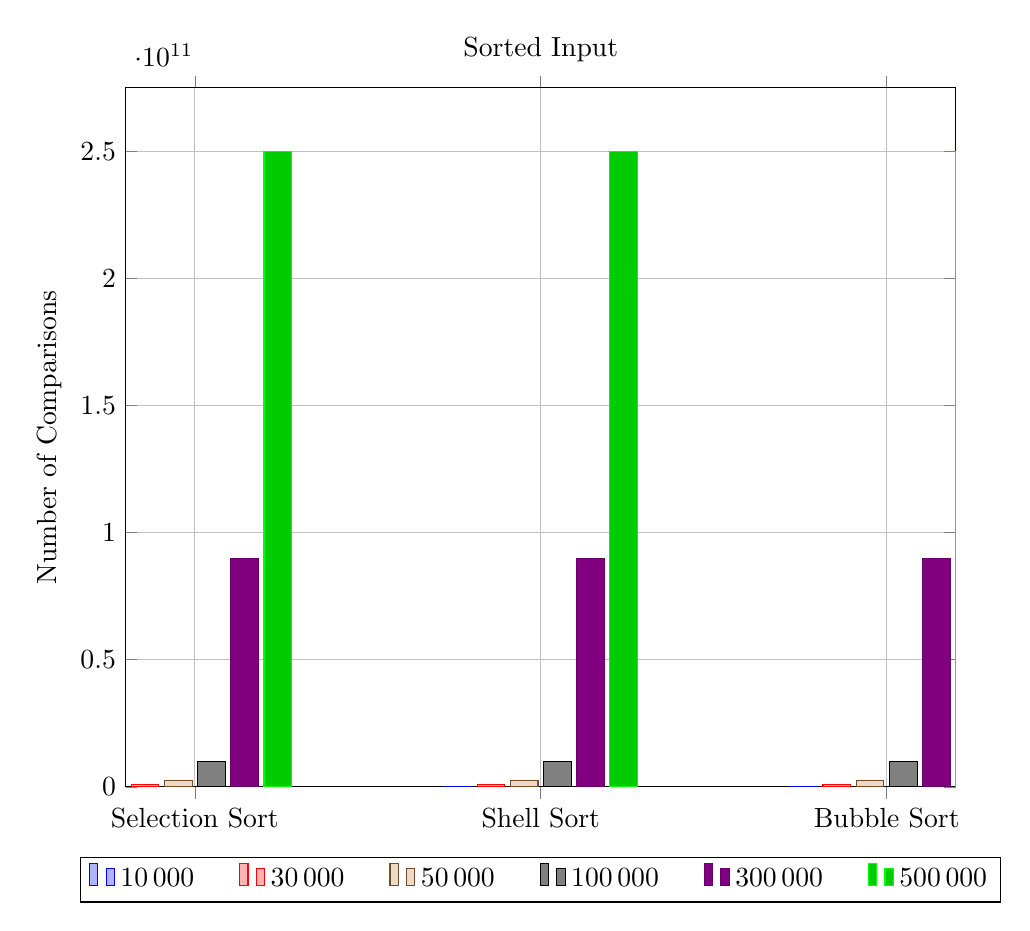
\begin{tikzpicture}
    \begin{axis}[
        width=\textwidth,
        title={Sorted Input},
        ybar,
        ymin=0,
        grid=major,
        legend style={
            at={(0.5,-0.1)}, anchor=north, legend columns=-1,
            /tikz/every even column/.append style={column sep=0.5cm}
        },
        ylabel={Number of Comparisons},
        symbolic x coords={Selection Sort, Shell Sort, Bubble Sort},
        xtick=data,
    ]
    \addplot coordinates {(Selection Sort,100009999) 
        (Shell Sort,100009999) (Bubble Sort,100009999)};
    \addplot coordinates {(Selection Sort,900029999) 
        (Shell Sort,900029999) (Bubble Sort,900029999)};
    \addplot coordinates {(Selection Sort,2500049999) 
        (Shell Sort,2500049999) (Bubble Sort,2500049999)};
    \addplot coordinates {(Selection Sort,10000099999) 
        (Shell Sort,10000099999) (Bubble Sort,10000099999)};
    \addplot coordinates {(Selection Sort,90000299999) 
        (Shell Sort,90000299999) (Bubble Sort,90000299999)};
    \addplot coordinates {(Selection Sort,250000499999) 
        (Shell Sort,250000499999) (Bubble Sort,250000499999)};
    \legend{10\,000, 30\,000, 50\,000, 100\,000, 300\,000, 500\,000}
    \end{axis}
\end{tikzpicture}
\caption{Kết quả thực nghiệm với đầu vào có thứ tự đã được sắp xếp (Nhóm 1)}
\end{figure}

\begin{figure}[H]
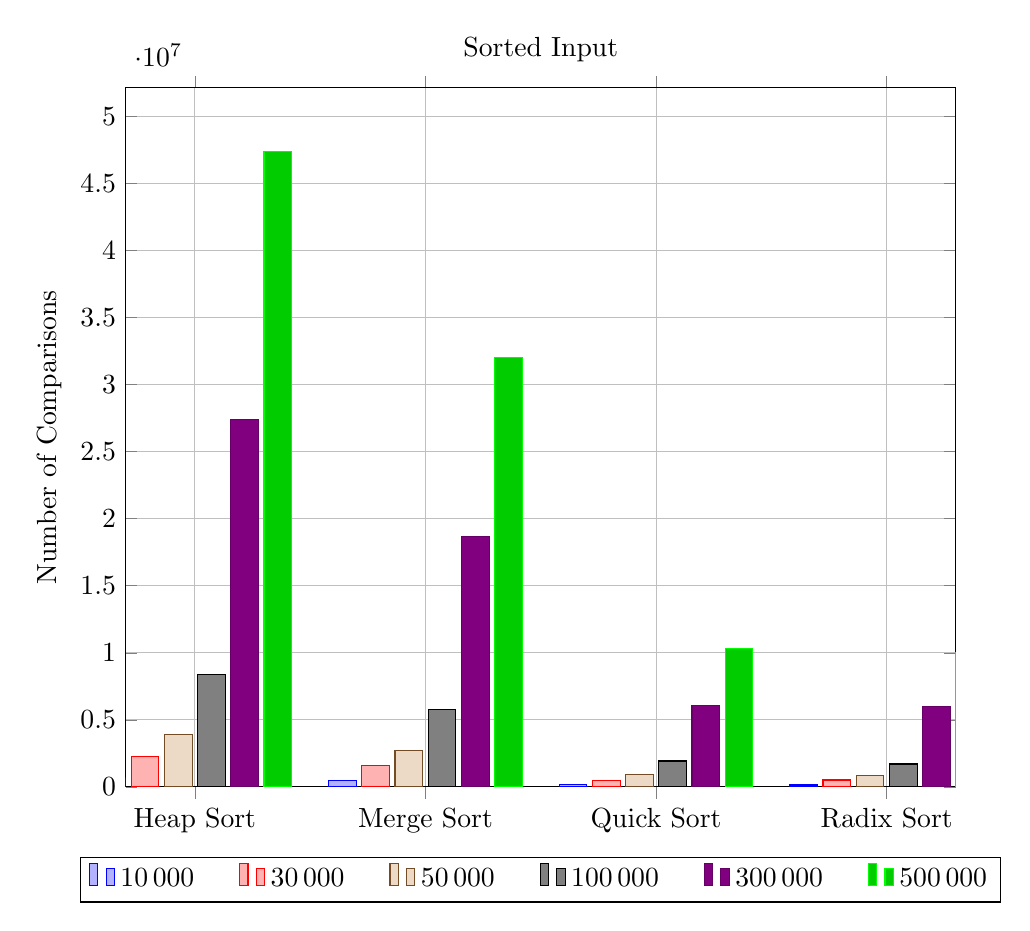
\begin{tikzpicture}
    \begin{axis}[
        width=\textwidth,
        title={Sorted Input},
        ybar,
        ymin=0,
        grid=major,
        legend style={
            at={(0.5,-0.1)}, anchor=north, legend columns=-1,
            /tikz/every even column/.append style={column sep=0.5cm}
        },
        ylabel={Number of Comparisons},
        symbolic x coords={Heap Sort, Merge Sort, Quick Sort, Radix Sort},
        xtick=data,
    ]
    \addplot coordinates {(Heap Sort,670329) (Merge Sort,475242) 
        (Quick Sort,154959) (Radix Sort,140056)};
    \addplot coordinates {(Heap Sort,2236648) (Merge Sort,1559914) 
        (Quick Sort,501929) (Radix Sort,510070)};
    \addplot coordinates {(Heap Sort,3925351) (Merge Sort,2722826) 
        (Quick Sort,913850) (Radix Sort,850070)};
    \addplot coordinates {(Heap Sort,8365080) (Merge Sort,5745658) 
        (Quick Sort,1927691) (Radix Sort,1700070)};
    \addplot coordinates {(Heap Sort,27413230) (Merge Sort,18645946) 
        (Quick Sort,6058228) (Radix Sort,6000084)};
    \addplot coordinates {(Heap Sort,47404886) (Merge Sort,32017850) 
        (Quick Sort,10310733) (Radix Sort,10000084)};
    \legend{10\,000, 30\,000, 50\,000, 100\,000, 300\,000, 500\,000}
    \end{axis}
\end{tikzpicture}
\caption{Kết quả thực nghiệm với đầu vào có thứ tự đã được sắp xếp (Nhóm 2)}
\end{figure}

\begin{figure}[H]
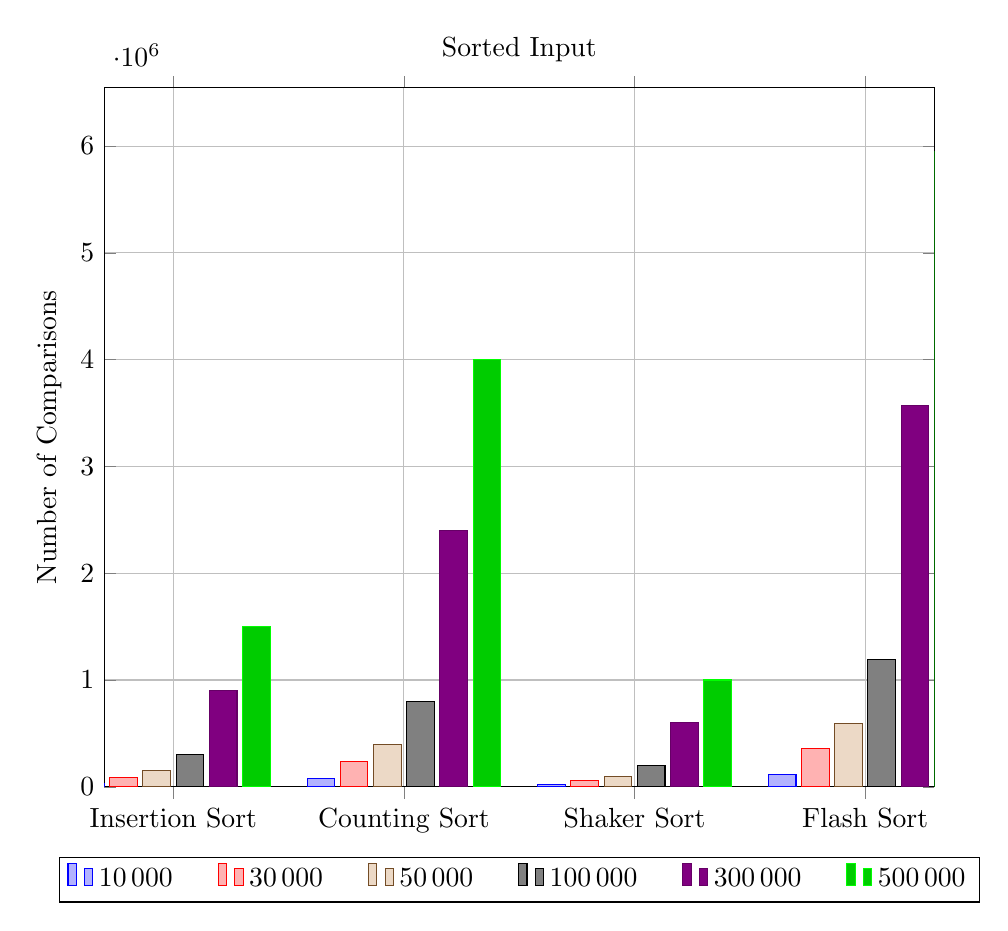
\begin{tikzpicture}
    \begin{axis}[
        width=\textwidth,
        title={Sorted Input},
        ybar,
        ymin=0,
        grid=major,
        legend style={
            at={(0.5,-0.1)}, anchor=north, legend columns=-1,
            /tikz/every even column/.append style={column sep=0.5cm}
        },
        ylabel={Number of Comparisons},
        symbolic x coords={Insertion Sort, Counting Sort, Shaker Sort, Flash Sort},
        xtick=data,
    ]
    \addplot coordinates {(Insertion Sort,29998) 
        (Counting Sort,80001) (Shaker Sort,20001) (Flash Sort,118993)};
    \addplot coordinates {(Insertion Sort,89998) 
        (Counting Sort,240001) (Shaker Sort,60001) (Flash Sort,356993)};
    \addplot coordinates {(Insertion Sort,149998) 
        (Counting Sort,400001) (Shaker Sort,100001) (Flash Sort,594993)};
    \addplot coordinates {(Insertion Sort,299998) 
        (Counting Sort,800001) (Shaker Sort,200001) (Flash Sort,1189993)};
    \addplot coordinates {(Insertion Sort,899998) 
        (Counting Sort,2400001) (Shaker Sort,600001) (Flash Sort,3569993)};
    \addplot coordinates {(Insertion Sort,1499998) 
        (Counting Sort,4000001) (Shaker Sort,1000001) (Flash Sort,5949993)};
    \legend{10\,000, 30\,000, 50\,000, 100\,000, 300\,000, 500\,000}
    \end{axis}
\end{tikzpicture}
\caption{Kết quả thực nghiệm với đầu vào có thứ tự đã được sắp xếp (Nhóm 3)}
\end{figure}

\begin{itemize}[label=$\circ$]
    \item Selection Sort, Shell Sort và Bubble Sort thực hiện một lượng 
    rất lớn số phép so sánh, đặc biệt là khi kích thước đầu vào lớn. Đó 
    là do các thuật toán này không có cách nào để “nhận ra” mảng đã được 
    sắp xếp xong nên liên tục thực hiện những phép so sánh vô nghĩa.
    \item Thuật toán Shaker Sort có số phép so sánh nhỏ nhất trong bảng 
    số liệu. Là một phiên bản cải tiến của Bubble Sort nên khi mảng đã 
    được sắp xếp sẵn, Shaker Sort chỉ cần duyệt qua mảng để xác nhận 
    rằng nó đã sắp xếp đúng, dẫn đến số phép so sánh rất thấp. Bên cạnh 
    đó, Insertion Sort cũng có số phép so sánh ít trong trường hợp mảng 
    đã được sắp xếp sẵn vì mỗi phần tử chỉ cần kiểm tra một lần với phần 
    tử liền trước để đảm bảo vị trí đúng mà không cần thực hiện thêm phép 
    so sánh nào khác.
\end{itemize}

$\bullet$ \textbf{Với đầu vào có thứ tự được sắp xếp ngược}

\begin{figure}[H]
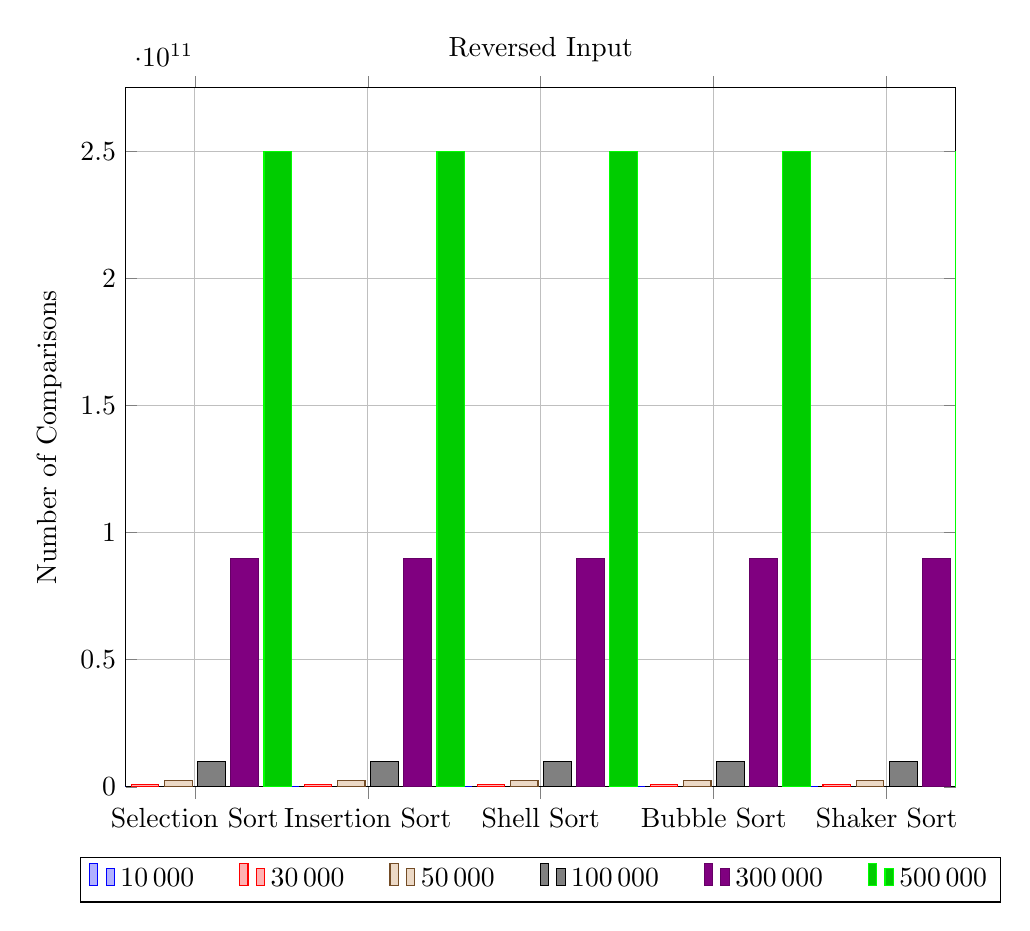
\begin{tikzpicture}
    \begin{axis}[
        width=\textwidth,
        title={Reversed Input},
        ybar,
        ymin=0,
        grid=major,
        legend style={
            at={(0.5,-0.1)}, anchor=north, legend columns=-1,
            /tikz/every even column/.append style={column sep=0.5cm}
        },
        ylabel={Number of Comparisons},
        symbolic x coords={Selection Sort, Insertion Sort, Shell Sort, Bubble Sort, Shaker Sort},
        xtick=data,
    ]
    \addplot coordinates {(Selection Sort,100009999) (Insertion Sort,100009999)
        (Shell Sort,100009999) (Bubble Sort,100009999) (Shaker Sort,100010001)};
    \addplot coordinates {(Selection Sort,900029999) (Insertion Sort,900029999)
        (Shell Sort,900029999) (Bubble Sort,900029999) (Shaker Sort,900030001)};
    \addplot coordinates {(Selection Sort,2500049999) (Insertion Sort,2500049999)
        (Shell Sort,2500049999) (Bubble Sort,2500049999) (Shaker Sort,2500050001)};
    \addplot coordinates {(Selection Sort,10000099999) (Insertion Sort,10000099999)
        (Shell Sort,10000099999) (Bubble Sort,10000099999) (Shaker Sort,10000100001)};
    \addplot coordinates {(Selection Sort,90000299999) (Insertion Sort,90000299999)
        (Shell Sort,90000299999) (Bubble Sort,90000299999) (Shaker Sort,90000300001)};
    \addplot coordinates {(Selection Sort,250000499999) (Insertion Sort,250000499999)
        (Shell Sort,250000499999) (Bubble Sort,250000499999) (Shaker Sort,250000500001)};
    \legend{10\,000, 30\,000, 50\,000, 100\,000, 300\,000, 500\,000}
    \end{axis}
\end{tikzpicture}
\caption{Kết quả thực nghiệm với đầu vào có thứ tự được sắp xếp ngược (Nhóm 1)}
\end{figure}

\begin{figure}[H]
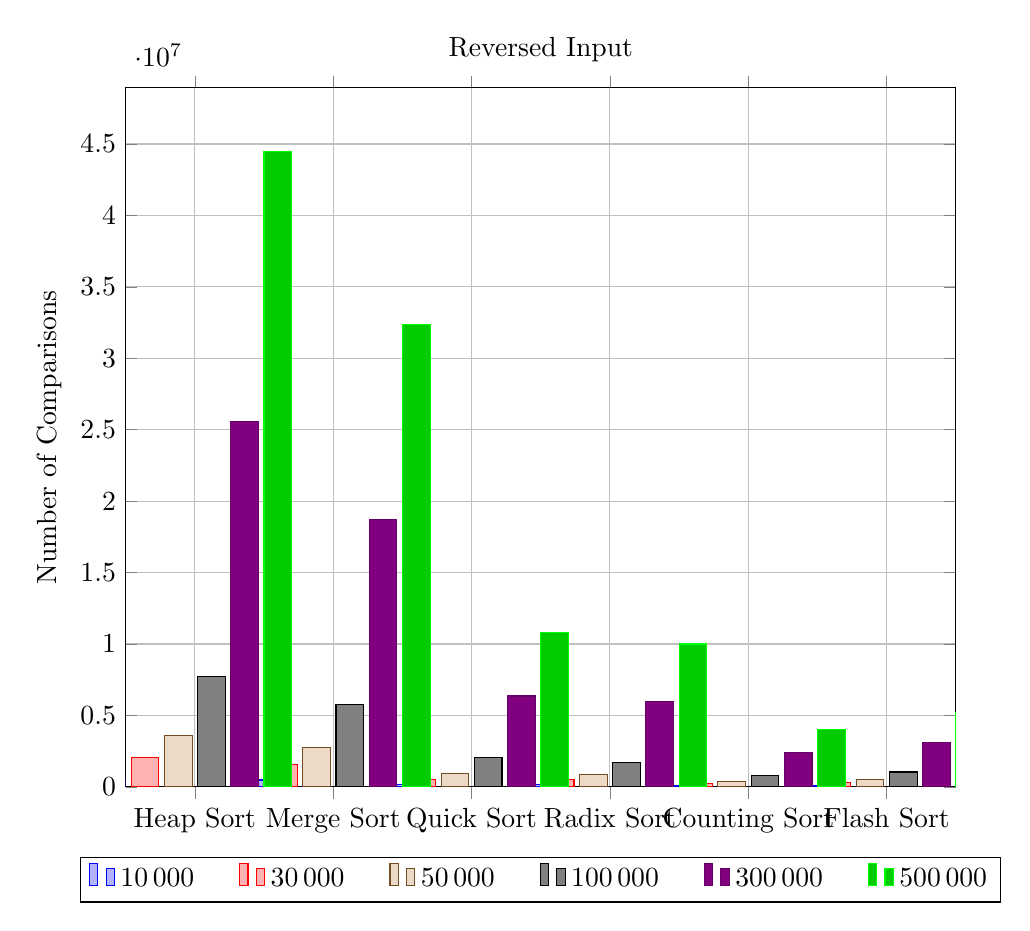
\begin{tikzpicture}
    \begin{axis}[
        width=\textwidth,
        title={Reversed Input},
        ybar,
        ymin=0,
        grid=major,
        legend style={
            at={(0.5,-0.1)}, anchor=north, legend columns=-1,
            /tikz/every even column/.append style={column sep=0.5cm}
        },
        ylabel={Number of Comparisons},
        symbolic x coords={Heap Sort, Merge Sort, Quick Sort, Radix Sort, Counting Sort, Flash Sort},
        xtick=data,
    ]
    \addplot coordinates {(Heap Sort,606771) (Merge Sort,476441) (Quick Sort,164975)
        (Radix Sort,140056) (Counting Sort,80001) (Flash Sort,103751)};
    \addplot coordinates {(Heap Sort,2063324) (Merge Sort,1573465) (Quick Sort,531939)
        (Radix Sort,510070) (Counting Sort,240001) (Flash Sort,311251)};
    \addplot coordinates {(Heap Sort,3612724) (Merge Sort,2733945) (Quick Sort,963861)
        (Radix Sort,850070) (Counting Sort,400001) (Flash Sort,518751)};
    \addplot coordinates {(Heap Sort,7718943) (Merge Sort,5767897) (Quick Sort,2027703)
        (Radix Sort,1700070) (Counting Sort,800001) (Flash Sort,1037501)};
    \addplot coordinates {(Heap Sort,25569379) (Merge Sort,18708313) (Quick Sort,6358249)
        (Radix Sort,6000084) (Counting Sort,2400001) (Flash Sort,3112501)};
    \addplot coordinates {(Heap Sort,44483348) (Merge Sort,32336409) (Quick Sort,10810747)
        (Radix Sort,10000084) (Counting Sort,4000001) (Flash Sort,5187501)};
    \legend{10\,000, 30\,000, 50\,000, 100\,000, 300\,000, 500\,000}
    \end{axis}
\end{tikzpicture}
\caption{Kết quả thực nghiệm với đầu vào có thứ tự được sắp xếp ngược (Nhóm 2)}
\end{figure}

\begin{itemize}[label=$\circ$]
    \item Selection Sort, Insertion Sort, Shell Sort, Bubble Sort và 
    Shaker Sort đều có số phép so sánh rất lớn trong trường hợp mảng được 
    sắp xếp ngược vì đây là trường hợp xấu nhất - mọi phần tử đều nằm sai 
    vị trí. Khi đó, các thuật toán này phải kiểm tra và điều chỉnh vị trí 
    của từng phần tử thông qua nhiều lần duyệt hoặc so sánh cặp.
    \item Counting Sort và Flash Sort có số phép so sánh khá ít trong 
    trường hợp này. Trong khi Counting Sort chỉ dựa trên việc đếm số lượng 
    phần tử trong các giá trị hoặc phạm vi thì Flash Sort sử dụng cách 
    phân chia mảng thành các nhóm dựa trên giá trị. Cả hai thuật toán này 
    đều hạn chế so sánh trực tiếp giữa các phần tử nên dù cho mảng có sắp 
    xếp ngược vẫn không ảnh hưởng quá nhiều.
\end{itemize}

$\blacktriangleright$ \textbf{Kết luận:}

[TO DO]
\pagebreak

\section{Một số lưu ý}
\pagebreak

% References
\nocite{*}
\cleardoublepage
\phantomsection
\addcontentsline{toc}{section}{Tài liệu tham khảo}
\bibliographystyle{unsrt}
\renewcommand{\refname}{Tài liệu tham khảo}
\bibliography{ref/ref}

\end{document}